\documentclass[a4paper, 10pt]{report}

%% Mandatory stuff
\usepackage[utf8]{inputenc}
\usepackage[T1]{fontenc}
\usepackage[french]{babel}

%% --
%% Bitstream Charter for text and maths
%% with ye Olde french typography
%% Note: fake small caps
%\usepackage[uppercase=upright,%
%  greeklowercase=upright,%
%  bitstream-charter]{mathdesign}
%% --
%% Math package
\usepackage{amsmath}
\usepackage{amssymb}
\usepackage{amsfonts}
\usepackage{mathrsfs}

\usepackage{graphicx}
\usepackage{float}

\usepackage{caption}
\usepackage{subcaption}

\usepackage{array}
\usepackage{multirow}

%% Color package for colored links
\usepackage[usenames]{color}

%% Hyperlinks for references, in color-O-vision
\usepackage[pdftex,%
  pdfauthor={DEMARE Thibaut},%
  pdftitle={Réseaux viaires et évacuation},%
  pdfsubject={Sujet},%
  colorlinks,%
  linkcolor=colHyperlinks,%
  urlcolor=colHyperlinks,%
  citecolor=colHyperlinks,
  plainpages=false]{hyperref}

%% Color for hyperlinks
\definecolor{colHyperlinks}{RGB}{0,90,170}%{59,0,159}

%% Code listings
\usepackage{listings}
%% Eye candy
%parametrage pour le style d'affichage du code source

%Version en noir et blanc
\definecolor{colKeys}{rgb}{0,0,0}%{0,0,1}
\definecolor{colIdentifier}{rgb}{0,0,0}
\definecolor{colString}{rgb}{0.6,0.6,0.6}
\definecolor{colComments}{RGB}{0,90,170}%\definecolor{colComments}{rgb}{0.4,0.4,0.4}

%Version couleur :
% \definecolor{colKeys}{RGB}{0,0,0}
% \definecolor{colIdentifier}{RGB}{50,50,50}
% \definecolor{colString}{RGB}{59,0,159}
% \definecolor{colComments}{RGB}{23,207,236}

\lstset{%configuration de listings
%Style generale de l'affichage
     float=hbp,%
     basicstyle=\normalsize, %\ttfamily
     identifierstyle=\color{colIdentifier}, %
     keywordstyle=\color{colKeys}\bf\normalsize, %
     stringstyle=\color{colString}, %
     commentstyle=\color{colComments}\normalsize\it, %
     columns=flexible, %
     tabsize=2, %
     frame=single, %
     extendedchars=true, %
     showspaces=false, %
     showstringspaces=true, %
     numbers=left, %
     numberstyle=\tiny, %
     breaklines=true, %
     breakautoindent=true, %
     captionpos=b,%
     xrightmargin=-3cm, %
     xleftmargin=-2cm,
% Permet l'utilisation de balise latex, dont le mode math
     texcl,
% Permet l'affichage d'accent dans le code source
     literate =
%   * Lettres a et A
      {à}{{\`a}}1 {â}{{\^a}}1
      {À}{{\`A}}1 {Â}{{\^A}}1
%   * Lettres c et C
      {ç}{{\c{c}}}1
      {Ç}{{\c{C}}}1
%   * Lettres e et E
      {é}{{\'e}}1 {è}{{\`e}}1 {ê}{{\^e}}1 {ë}{{\"e}}1
      {É}{{\'E}}1 {È}{{\`E}}1 {Ê}{{\^E}}1 {Ë}{{\"E}}1
%   * Lettres i et I
      {î}{{\^i}}1 {ï}{{\"i}}1
      {Î}{{\^I}}1 {Ï}{{\"I}}1
%   * Lettres o et O
      {ô}{{\^o}}1
      {Ô}{{\^O}}1
%   * Lettres u et U
      {ù}{{\`u}}1 {û}{{\^u}}1 {ü}{{\"u}}1
      {Ù}{{\`U}}1 {Û}{{\^U}}1 {Ü}{{\"U}}1
}
%environnement pour langage oriente objet
\lstnewenvironment{C++}{%
            \lstset{language=C++
               %permet de modifier l'affichage du code source selon le langage
               %,identifierstyle=\color{blue},keywordstyle=\color{Ckeywords},backgroundcolor=\color{Cbckgd}
                    }}{}
\lstnewenvironment{java}{%
            \lstset{language=Java}
                        }{}
%environnement pour langage web
\lstnewenvironment{php}{%
            \lstset{language=PHP}
                       }{}
\lstnewenvironment{html}{%
            \lstset{language=HTML}
                        }{}
%environnement pour langage SQL
\lstnewenvironment{sql}{%
            \lstset{language=SQL}
                       }{}
%environnement pour langage fonctionnel
\lstnewenvironment{caml}{%
            \lstset{language=Caml}
                       }{}
\lstnewenvironment{lisp}{%
            \lstset{language=Lisp}
                       }{}
\lstnewenvironment{lisp-term}{%
            \lstset{language=Lisp, backgroundcolor=\color{black}, basicstyle=\ttfamily\small\color{white}}
                       }{}
%autre langage
\lstnewenvironment{make}{%
            \lstset{language=make}
                       }{}
%langage algorithmique
\lstdefinelanguage{algo}{
    keywords={plap, tant, que, fin, faire, si, alors, allant, fonction, fonctions, disponibles, sinon, afficher, pour, chaque, sortie, plop},
    comment=[l]//,
    morecomment=[l]//,
    morecomment=[s]{/*}{*/},
    morestring=[b]",
    mathescape= true,
    sensitive=false,
    literate=
%   * Definition des operateurs avec un style mathematique
      {=}{{$\gets$}}1 {==}{{=}}1 {!=}{{$\neq$}}1
      {<=}{{$\leq$}}1 {>=}{{$\geq$}}1
%   * Definition du mot cle debut avec un accent. Il ne peut etre defini avec keywords car l'accent pose probleme 
      {début}{{\color{colKeys}\bf\normalsize d\'ebut}}1
      {Début}{{\color{colKeys}\bf\normalsize D\'ebut}}1
      {DÉBUT}{{\color{colKeys}\bf\normalsize D\'EBUT}}1      
%   * Definition du mot cle entree avec un accent. Il ne peut etre defini avec keywords car l'accent pose probleme 
      {entrée}{{\color{colKeys}\bf\normalsize entr\'ee}}1
      {Entrée}{{\color{colKeys}\bf\normalsize Entr\'ee}}1
      {ENTRÉE}{{\color{colKeys}\bf\normalsize ENTR\'EE}}1  
%   * Definition du mot cle donnees avec un accent. Il ne peut etre defini avec keywords car l'accent pose probleme 
      {données}{{\color{colKeys}\bf\normalsize donn\'ees}}1
      {Données}{{\color{colKeys}\bf\normalsize Donn\'ees}}1
      {DONNÉES}{{\color{colKeys}\bf\normalsize DONN\'EES}}1
%   * Redefinition des lettres accentuees car la definition precedente aura ecrase ces valeurs
%   * Lettres a et A
      {à}{{\`a }}1 {â}{{\^a}}1
      {À}{{\`A }}1 {Â}{{\^A}}1
%   * Lettres c et C
      {ç}{{\c{c}}}1
      {Ç}{{\c{C}}}1
%   * Lettres e et E
      {é}{{\'e}}1 {è}{{\`e}}1 {ê}{{\^e}}1 {ë}{{\"e}}1
      {É}{{\'E}}1 {È}{{\`E}}1 {Ê}{{\^E}}1 {Ë}{{\"E}}1
      {œ}{{\oe}}1 {Œ}{{\OE}}1
%   * Lettres i et I
      {î}{{\^i}}1 {ï}{{\"i}}1
      {Î}{{\^I}}1 {Ï}{{\"I}}1
%   * Lettres o et O
      {ô}{{\^o}}1
      {Ô}{{\^O}}1
%   * Lettres u et U
      {ù}{{\`u}}1 {û}{{\^u}}1 {ü}{{\"u}}1
      {Ù}{{\`U}}1 {Û}{{\^U}}1 {Ü}{{\"U}}1
}
\lstnewenvironment{algo}{%
            \lstset{language=algo}
                       }{}
%pour le langage des machines a registre
\lstdefinelanguage{RAM}{%
    morekeywords={plop, read, write, load, store, jz, decr, incr, jump, stop, plop}
    comment=[l]//,
    morecomment=[l]//,
    morecomment=[s]{/*}{*/},
    mathescape= true,
    sensitive=false
}
\lstnewenvironment{RAM}{%
            \lstset{language=RAM, firstnumber=0}
                       }{}

%% --
\usepackage{makeidx}
\makeindex

%% Plain page headings
\pagestyle{headings}

%% Smaller space between heading and matter
\setlength\headsep{0.5in}

% gere les chapitre non numeroté
\newcommand{\chaptertoc}[1]{\chapter*{#1}
\addcontentsline{toc}{chapter}{#1}
\markboth{\slshape\MakeUppercase{#1}}{\slshape\MakeUppercase{#1}}}

\usepackage{tikz,times}

\usetikzlibrary{mindmap,backgrounds}
\usepackage[absolute]{textpos}

\begin{document}

%
% Page de garde
%
\begin{titlepage}
	\setlength{\leftmargin}{0cm}
	\setlength{\rightmargin}{0cm}
	\setlength{\marginparwidth}{0cm}
	\setlength{\voffset}{0cm}

	\begin{center}
		\begin{textblock}{150}(3,3)
			\begin{flushleft}
				\begin{large}
					Université du Havre\\
					Master deuxième année\\
					Informatique
				\end{large}
			\end{flushleft}
		\end{textblock}
			
		\makebox[\textwidth]{
				\begin{tikzpicture}
					\definecolor{couleurUnie}{RGB}{0,129,188}
		
					\path[mindmap, concept color=couleurUnie,text=black, ]
					node[concept, fill=white, minimum size=170pt] at (0,0) {
						\centering
							\Huge{Réseaux viaires et \mbox{évacuation} } 
					}
						child[grow=75, concept color=couleurUnie, level distance=200] {
							node[concept, fill=white, minimum size=75] {\large{\textit{Auteur}} }
								child[grow=30, concept color=couleurUnie, level distance=100] { 
									node[concept, fill=white, minimum size=75] { \large{\textbf{Thibaut Démare}} } 
								}
						}
						child[grow=-75, concept color=couleurUnie, level distance=220] {
							node[concept, fill=white, minimum size=75] { \large{\textit{Date}} }
								child[grow=-30, concept color=couleurUnie, level distance=100] { 
									node[concept, fill=white, minimum size=75] { \large{\textbf{\today}} }
								} 
						}
						child[grow=-135, concept color=couleurUnie, level distance=200] {
							node[concept, fill=white, minimum size=75] {\large{\textit{Encadrants}}}
								child[grow=-45, concept color=couleurUnie, level distance=100] {
									node[concept, fill=white, minimum size=75] { \large{\textbf{Antoine Dutot}} }
								}
								child[grow=-135, concept color=couleurUnie, level distance=100] { 
									node[concept, fill=white, minimum size=75] { \large{\textbf{Damien Olivier}} } 
								} 
						};
				\end{tikzpicture}
		}
	\end{center}
\end{titlepage}


\newpage

\chapter*{Remerciements}

\paragraph{}Je tiens tout d'abord à remercier mes deux encadrants MM. Antoine \textsc{Dutot} et Damien \textsc{Olivier} qui se sont montrés présents et à l'écoute. Ils ont été de bons conseillers dans mes choix et c'est sans nulle doute grâce à eux que nous traitons ici de fourmis.

\paragraph{}Je souhaite également exprimer toute ma gratitude aux membres du laboratoire du Litis qui ont été très accueillants pendant ces quatre mois. Je tiens d'ailleurs à témoigner ma reconnaissance envers M. Cyrille \textsc{Bertelle} qui a bien voulu accepter ma candidature pour une thèse l'année prochaine.

\paragraph{}Bien sûr je ne saurais oublier mes camarades de stage avec qui l'ennui ne s'est jamais fait sentir. Que ce soit lors des discussions sur les jeux vidéo, sur les films, lors de celles plus sérieuses sur nos sujets respectifs, ou lors de cette mémorable randonnée à Étretat et son GR21, j'ai toujours passé des moments très appréciables. Dans l'ordre alphabétique de leur prénom je cite ainsi Alexis, Florent, Guillaume, Merwan et Mohamed Ali. 
Toutefois, désolé à ceux qui se reconnaîtront que nous n'ayons pas plus parler de moustaches.

\paragraph{}Un grand merci également, et non des moindres, à Xavière et à mes parents pour partager ma passion de l'informatique alors que ce n'est pas forcément leur tasse de thé au départ.

\paragraph{}Et pour finir, merci au lecteur qui passera par là et accordera un peu de son temps pour lire ces quelques pages.

\tableofcontents

\newpage

\chaptertoc{Abstract}

\paragraph{}The mesh of a road network can be very complex to understand, to analyze. Its particular topology is first a positive point because it allows  good accessibility for users, but it can be a weakness if we route an important mass of vehicles on the same road. Tunnels, bridges, highways, interchanges are structures intended to facilitate transport, but they can become quite the bottlenecks when good or bad conditions are presents.

\paragraph{}In order to identify these critical zones, the betweenness centrality can be used. It provides a measure on nodes of a graph by computing, for each node $v$, the number of shortest paths passing through $v$ among all possible shortest paths of the graph.

This way, when a significant amount of paths traverse a set of nodes, we emphasize major road segments able to handle a large traffic. 

\paragraph{}If a part of the network becomes inaccessible because of, for example, an industrial accident, and if we wish do an evacuation, then it is useful to know the state of the betweenness centrality in order to provide adapted routes and avoid creating a bottleneck.
However, the algorithm is very slow and very expensive to compute. Depending on the size of the graph taken into account, it can be unpractical to recompute all shortest paths at each change.

\paragraph{}Thus, the purpose of this report is to present a computing method for the centrality, allowing real-time updates under acceptable delays.
To answer to this problematic, we suggest robust methods for this dynamic.

\paragraph{}The first model is derived from a hypothesis that the betweenness centrality and a random walk can be correlated. It was an observation from Michel Nabaa's thesis where the coloration of the road network of Le Havre according to these two methods seemed to emphasize the same areas.

\paragraph{}The use of our comparatives measures, \textit{e.g.} Pearson's and Spearman's correlation coefficients, have proved the contrary when we have repeated the experience.

\paragraph{}So, we have designed a second model closer to the original definition. This one is inspired by Brandes' model using pivot nodes. His algorithm solves all shortest paths from these pivot sources to all the other nodes. For our part, we have chosen to select directly a subset of pairs of nodes rather than to prefer some sources in particular. With the intention of solving the path problem between the nodes of each pair, we have used some entities whose behavior is to find a solution.

\paragraph{}The first entity executes a random walk and increments a counter when it crosses a node or an edge. It also deletes the cycle in the path. Unfortunately, the correlation between the centrality and this counter does not exist on some graphs but exists on some other types. In this particular case, the results are not positive on the road networks of two French cities, Le Havre and Rouen, even if we use a biased random walk.

\paragraph{}Then, we wanted to prove the viability of our model with an entity using the A$^*$ algorithm. The latter allows to compute efficiently a shortest path between two nodes of a graph. Our comparative measures gave us positive results since there is a strong correlation between the betweenness centrality and our model.

\paragraph{}However, the A$^*$ algorithm can not be applied in the general case because of the heuristics needed. Therefore, we have designed a final entity based on Dorigo's ants. It is a method inspired by the stigmergy where entities coordinate indirectly their actions through the environment and pheromones.

\paragraph{}In our model, a master process holds a list of pairs of nodes, and we associate to each pair a different type of pheromone. During the computation, the master process orders the colony to make a path between the source and the destination of a given pair. The entities solve their problem and put down the pheromones on their computed path. The quantity depends on the length of the path.

Since the entities are sensible to the pheromone when they move, they will prefer to choose the shortest path a little more at each step.

\paragraph{}Although we have just one result at this time for this model of ant entities, this method is promising and can provide some interesting results in the general case.

\paragraph{}However, it is necessary to optimize again the mechanism of the ant entity because it still does not work perfectly on the road network. Furthermore, the method of selection of pairs can surely be improved by a most elaborated mechanism. We can imagine, for example, that we choose the nodes between different clusters determined by a clustering algorithm.

\paragraph{}The number of pairs used is also an important parameter of our model but we have not defined his ideal value. Thus, it is an interesting prospect to implement, along with the distribution of our algorithm.

%
% Résumé en version française
%
% \paragraph{}Le maillage d'un réseau routier peut se montrer très complexe à comprendre, à analyser. Sa topologie particulière est d'abords une force car elle permet l'accessibilité aux usagers, mais peut être une faiblesse quand nous nous employons à acheminer une masse importante de véhicules sur une même voie. Les tunnels, les ponts, les autoroutes, les échangeurs sont autant de structures pour faciliter le transport que de véritables goulots d'étranglement quand les bonnes conditions se présentent.

% \paragraph{}Afin d'identifier ces zones critiques, la centralité intermédiaire peut être utilisée. Elle fournit une mesure aux n\oe uds d'un graphe en calculant pour chaque n\oe ud $v$ le nombre de plus courts chemins passant par $v$ parmi tout les plus courts chemins possibles d'un graphe. 

%Ainsi nous mettons en valeur le axes susceptibles d'être très empruntée car une quantité importante de chemins transite par là.
% 
% \paragraph{}Si une partie du réseau est rendu inaccessible à cause, par exemple, d'un accident industriel, et que nous souhaitons faire une évacuation, alors il est utile de connaître l'état de la centralité intermédiaire pour fournir des itinéraires adaptés et éviter de créer des goulots d'étranglement. Toutefois, ce calcul est très long et très coûteux. Selon la taille du réseau pris en compte, il peut être impossible de recalculer tout les plus courts chemins à chaque changement.
% 
% \paragraph{}Ainsi, l'objet de ce rapport est de présenter une méthode de calcul de la centralité rendant possible la mise à jour de la mesure dans un délai acceptable. Nous avons souhaité répondre à cette problématique en proposant des modèles robustes à la dynamique.
% 
% \paragraph{}Le premier modèle proposé est issue d'une hypothèse de départ que la centralité intermédiaire et une marche aléatoire peut être corrélé. Il s'agissait d'un constat d'après la thèse Michel Nabaa où la coloration du réseau routier du Havre d'après ces deux méthodes semblait mettre en valeur les même zones.
% 
% \paragraph{}Les méthodes d'analyses employées, c'est à dire les coefficients de corrélation de Pearson et de Spearman nous ont prouvé le contraire lorsque nous avons refait l'expérience.
% 
% \paragraph{}Nous avons ainsi conçu un second modèle plus proche de la définition initiale. Celui-ci est inspiré du modèle de Brandes utilisant des n\oe uds pivots. Son algorithme résout tout les plus courts chemins vers tout les autres n\oe uds à partir de ces sources pivots. Nous avons quant à nous choisi de sélectionner directement un sous ensemble de paires de n\oe uds plutôt que de préférer des n\oe uds sources. Pour résoudre les chemins entre ces paires, nous avons utilisé des entités dont le comportement doit permettre ce calcul. 
% 
% \paragraph{}La première entité effectue une marche aléatoire mais la corrélation n'était au rendez-vous que sur certains graphes. En l'occurrence, cela ne donnait pas de résultats concluant sur les réseaux viaires du Havre et de Rouen même en utilisant des marches aléatoire biaisées.
% 
% \paragraph{}Ensuite nous avons voulu prouver la viabilité du modèle avec des entités utilisant A$^*$. Cet algorithme permet de calculer efficacement un plus court chemin entre deux n\oe uds d'un graphe. Les méthodes d'analyses nous ont ainsi rassuré puisqu'il en résulte une forte corrélation entre la centralité intermédiaire et notre modèle.
% 
% \paragraph{}Puisque l'algorithme A$^*$ ne peut s'appliquer dans le cas général, nous avons ensuite proposer une entité basée sur les fourmis de Dorigo. Il s'agit d'un principe inspiré de la stigmergie où les entités communiquent via des phéromones qu'elles posent sur leur environnement; dans notre cas les arêtes du graphe font office d'environnement.
% 
% \paragraph{}Un processus maître détient une liste de paires de n\oe uds dont nous associons à chacune un type de phéromone différent. Au cours du calcul, il ordonne à la colonie de se rendre du n\oe ud de départ à la destination définis par la paire courante. Les entités résolvent leur problème puis déposent des phéromones sur leur chemin en quantité dépendant de la longueur de celui-ci. 
% 
% Puisqu'elles sont sensibles à la phéromone pour se déplacer, elles seront à chaque passage orientées un peu plus vers le plus court chemin.
% 
% \paragraph{}Bien que nous n'ayons qu'un seul résultat pour le moment concernant cette entité, le modèle est prometteur et peut fournir des résultats intéressant dans le cas général.
% 
% \paragraph{}Il est toutefois nécessaire d'optimiser encore le fonctionnement de l'entité fourmi. De plus, le mode de sélection des paires peut sûrement être amélioré par un mécanisme plus élaboré. Nous pouvons imaginer par exemple choisir les n\oe uds contenu dans des clusters différents pour constituer les paires. Nous devrons alors proposer une méthode de clustering. 
% 
% \paragraph{}Le nombre de paires utilisées est également un paramètre important de notre modèle mais nous n'avons pas défini sa valeur idéale. Il s'agit là encore d'une perspective à mettre en \oe uvre tout comme le serait la distribution de notre algorithme.


%%%%%%%%%%%%%%%%
% Introduction %
%%%%%%%%%%%%%%%%
\chaptertoc{Introduction}

\paragraph{}Afin de rester compétitif et attractif, une ville doit se doter d'un réseau routier efficace où l'optimisation des temps de transport est recherché. Pour cela, il peut être décidé de créer des axes principaux sur lesquels les vitesses de déplacement et le volume du trafic sont importants.

\paragraph{}Toutefois, en donnant une importance à certaines routes, cela risque de créer de véritables goulots d'étranglement. Effectivement, les risques industriels ou les accidents de la route peuvent bloquer ces axes et ainsi paralyser le trafic en très peu de temps. Il devient donc primordial d'étudier les réseaux viaires afin de mettre en valeur les zones sensibles pour comprendre comment améliorer ceux-ci et éviter des catastrophes en cas d'évacuation.

\paragraph{}Grâce à la théorie des graphes, nous pouvons effectuer des mesures précises sur le réseau pour déterminer sa robustesse et sa résilience. La centralité intermédiaire est l'un de ces indices. Elle se base sur les plus courts chemins entre toutes les paires de n\oe uds d'un graphe et elle permet justement de répondre à nos attentes. Malheureusement, cette mesure possède un important défaut : son temps de calcul. Par conséquent, si le graphe traité est dynamique, alors il devient très délicat de recalculer tous les plus courts chemins à chaque changement.

\paragraph{}Ainsi, au cours de ce rapport, nous nous proposons d'étudier la centralité intermédiaire puis de fournir une méthode de calcul robuste à la dynamique d'un graphe.

\paragraph{}Dans une première partie, nous présenterons en détail notre problème en montrant l'intérêt de calculer la centralité intermédiaire et en particulier dans le contexte dynamique.

\paragraph{}Par la suite nous détaillerons l'état de l'art concernant la centralité intermédiaire : l'approche classique mais également les méthodes dérivées dont certaines approximent le résultat réel, tandis que d'autres considèrent la recherche des chemins de façon complètement différente.

\paragraph{}En deuxième partie, nous considérerons les méthodes d'analyses qui vont nous servir à comparer nos modèles à la centralité classique.

\paragraph{}Dans la troisième partie, nous approfondirons notre première approche basée sur des marches aléatoires classiques. Nous verrons notamment que la méthode donne des résultats éloignés de la centralité intermédiaire.

\paragraph{}Ainsi la quatrième partie sera consacrée à un nouveau modèle, plus prometteur, qui se fonde sur un concept de paires de n\oe uds dit "pivots". 

\paragraph{}Finalement, nous explorerons les perspectives d'améliorations avant de conclure.

\chapter{Le problème}

\paragraph{}L'agglomération havraise est un système complexe dans lequel des entités hétérogènes cohabitent. Mais cela ne se fait pas toujours sans risques ni sans accidents. Le danger est bien présent et dans le but de le limiter ou même de le maîtriser, les collectivités locales ont financé des travaux de recherches pour trouver des solutions. 

\paragraph{}C'est dans cet objectif que Michel Nabaa a effectué sa thèse \cite{Nabaa2011Morphodyn}. Au cours de son travail, il a utilisé différentes méthodes pour mettre en valeur la robustesse et la résilience du réseau viaire du Havre.

\paragraph{}Pourtant la dynamique du système de cet espace géographique implique qu'une crise peut survenir très rapidement. Il est donc nécessaire de réagir promptement. Si un axe majeur se trouve bloqué car il mène ou il appartient à une zone de danger, alors il faut redéfinir les nouveaux axes majeurs. Cela permet de conseiller des itinéraires pour fluidifier le trafic au maximum et facilite une évacuation sans encombres.

\paragraph{}La théorie des graphes nous offre des mesures sur ceux ceux-ci nous permettant d'évaluer l'importance de certains n\oe uds ou arcs, au sens de la connectivité avec par exemple les points d'articulations, au sens de la transitivité comme avec le coefficient de clustering, ou encore au sens des plus courts chemins comme avec la centralité intermédiaire. C'est donc sur cette dernière que nous allons orienter notre travail.

\paragraph{}Malheureusement, c'est une mesure longue et coûteuse à calculer. Ainsi, nous souhaitons trouver une méthode palliant ces problèmes. Le sujet de ce stage consiste donc à trouver une méthode de calcul de la centralité qui soit rapide, ou permette de résister à la dynamique. De plus, pour minimiser les temps de calcul nous souhaitons favoriser les méthodes distribuables.

\chapter{La centralité intermédiaire}

\paragraph{}Les mesures de centralité dans un graphe sont des indicateurs locaux de la position d'un n\oe ud ou d'un arc dans le graphe. Les définitions de centralité sont toutefois nombreuses. Nous pouvons rencontrer par exemple la centralité de degré (le degré d'un n\oe ud), la centralité de proximité \cite{Sadibussi1966Centrality} (l'inverse de la somme de la la longueur des plus courts chemins entre chaque n\oe ud du graphe), la centralité d'éloignement maximal (la distance maximale entre un n\oe ud et l'ensemble des autres n\oe uds), et la centralité intermédiaire ou d'intermédiarité (voir figure \ref{fig:centralities}).

\begin{figure}[htbp]
	\centering
	\subcaptionbox{Centralité de degré.}[0.49\linewidth][c]{
		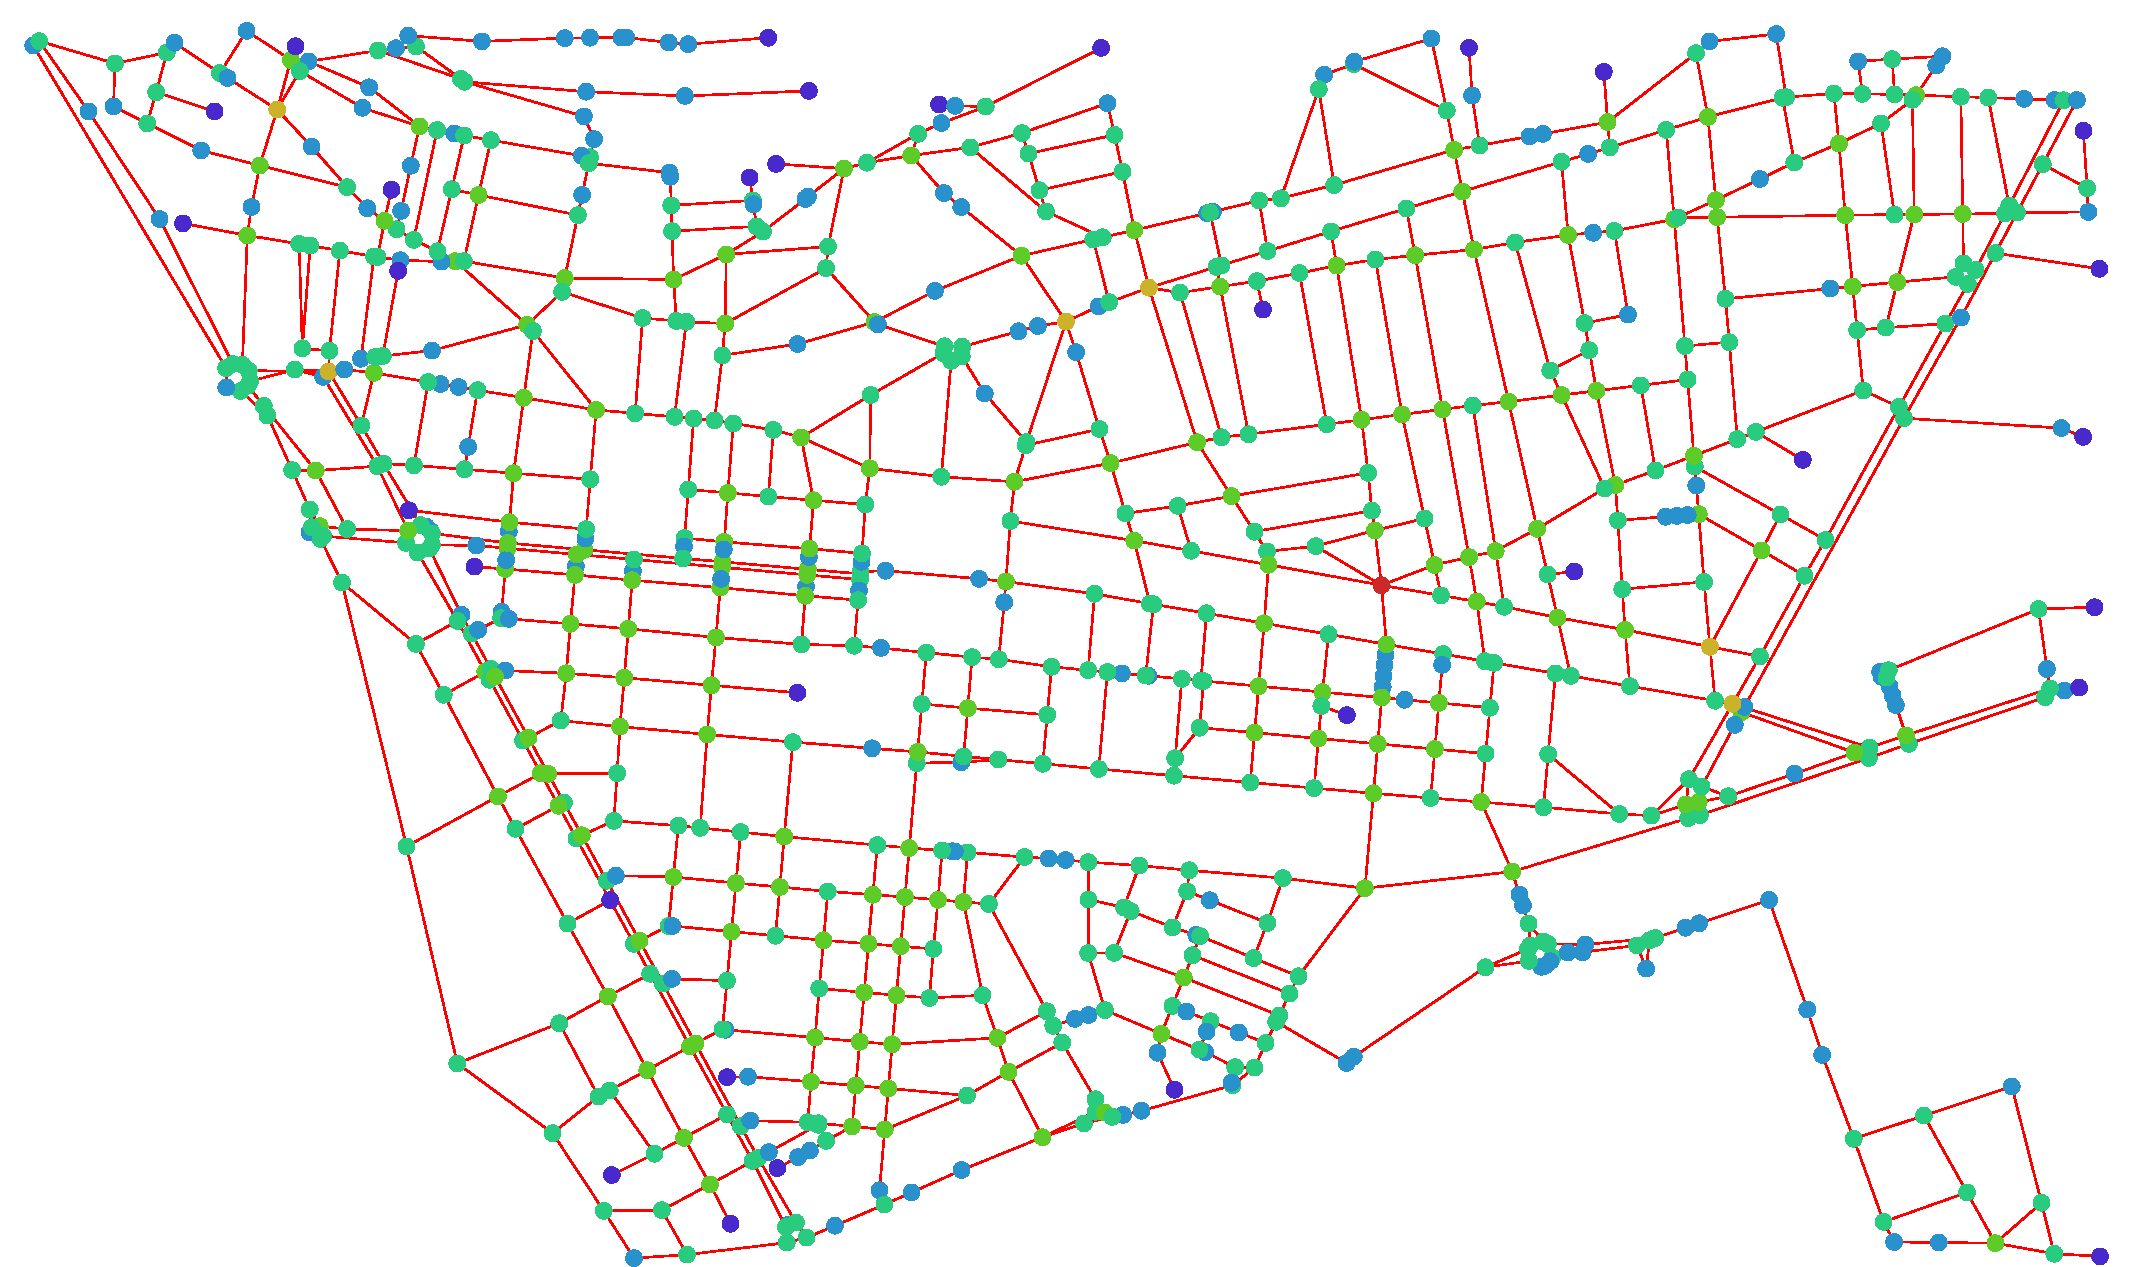
\includegraphics[width=0.49\linewidth]{./img/degree_centrality.pdf}
	}
	\hfill
	\subcaptionbox{Centralité d'éloignement maximal.}[0.49\linewidth][c]{
		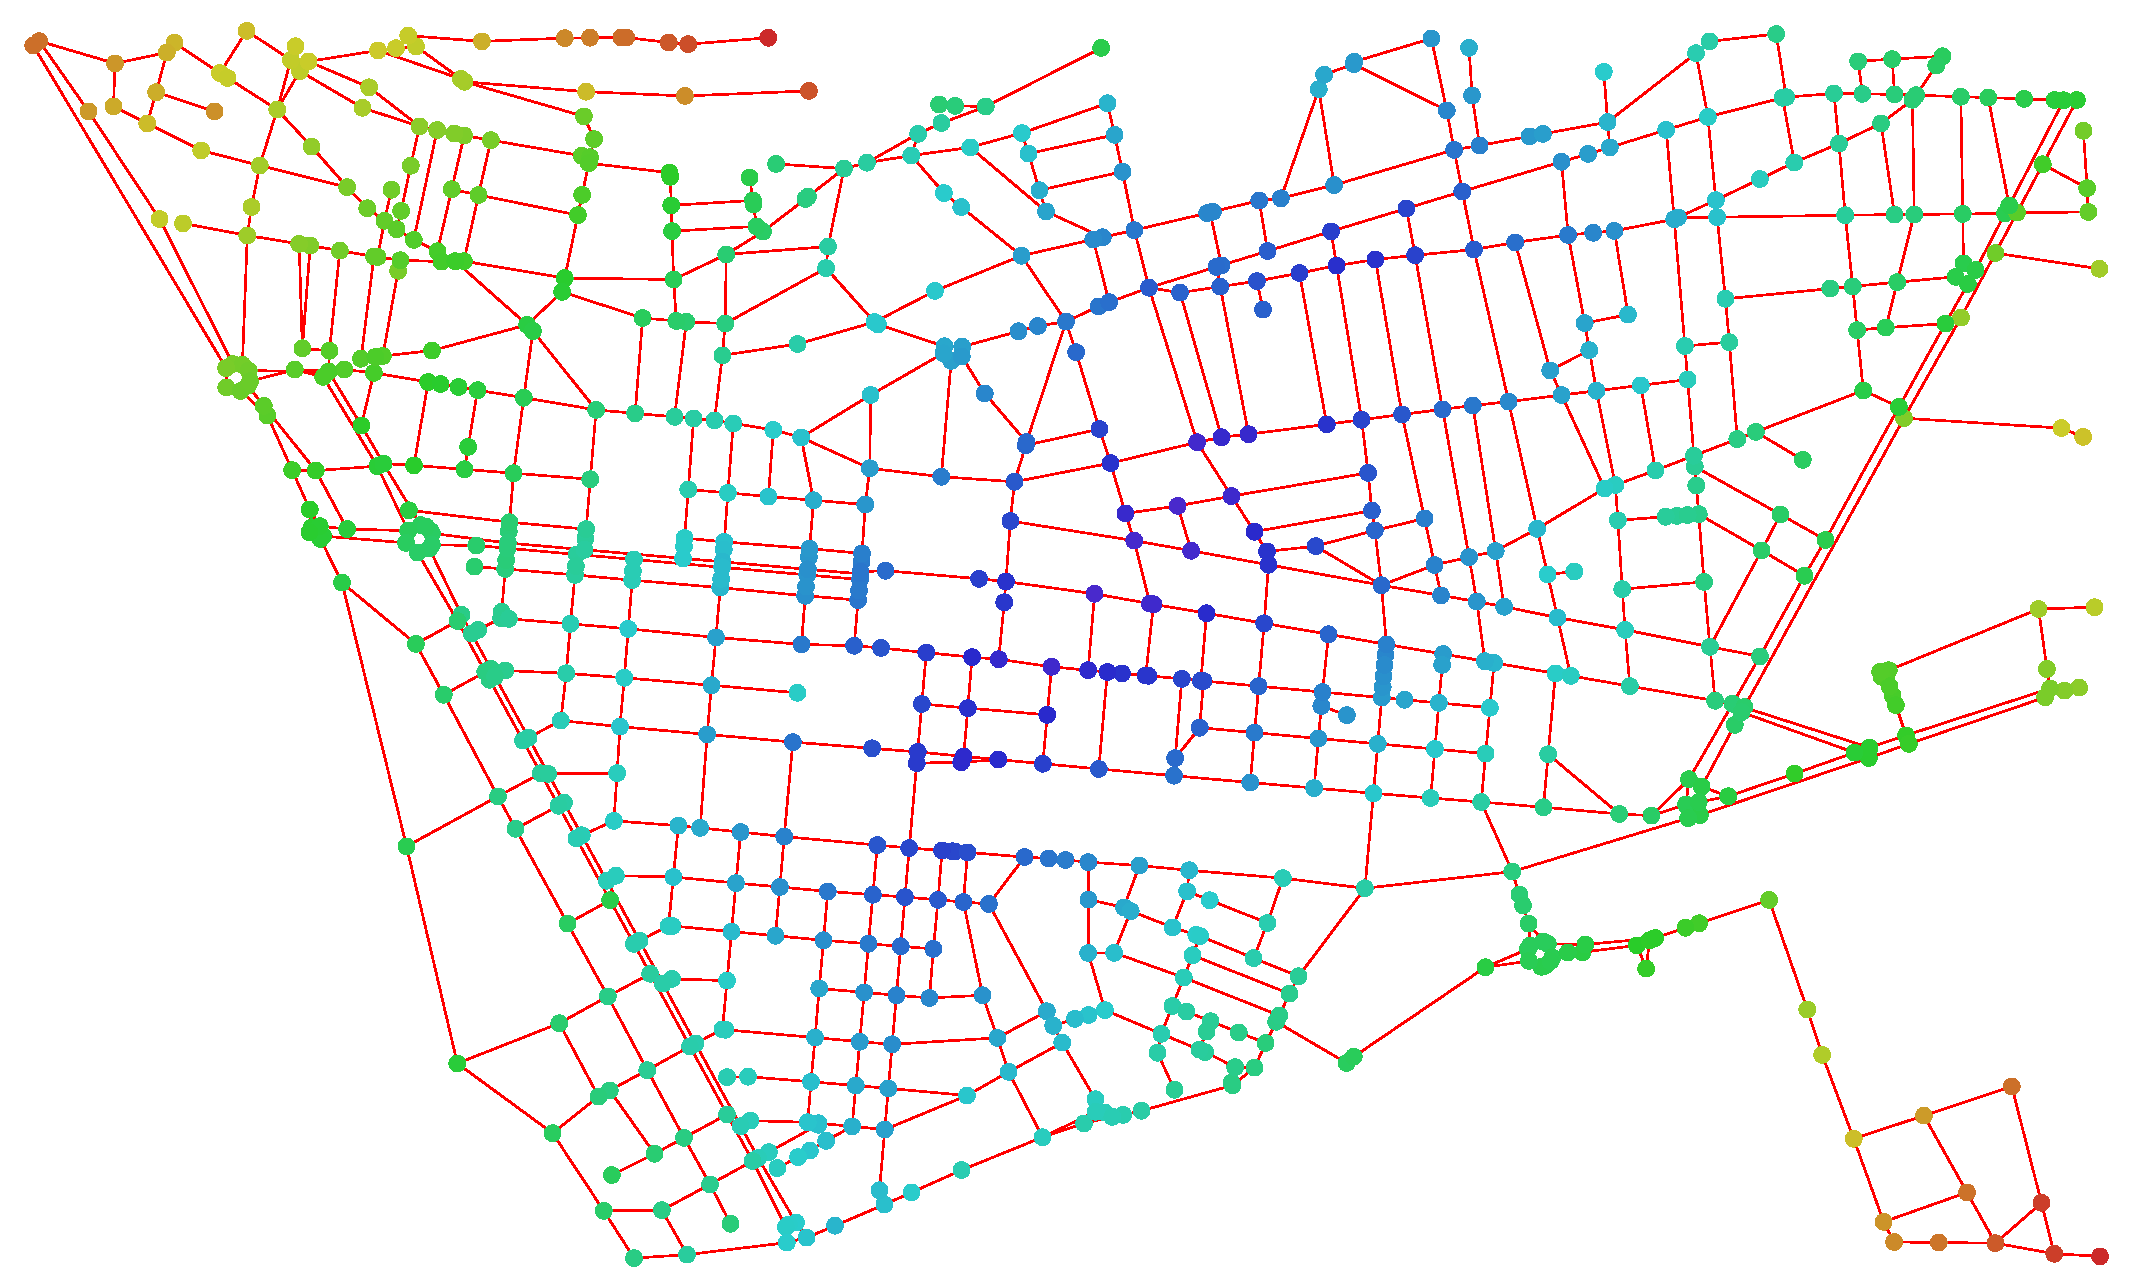
\includegraphics[width=0.49\linewidth]{./img/max_farness_centrality.pdf}
	}
	\hfill
	\subcaptionbox{Centralité de proximité.}[0.49\linewidth][c]{
		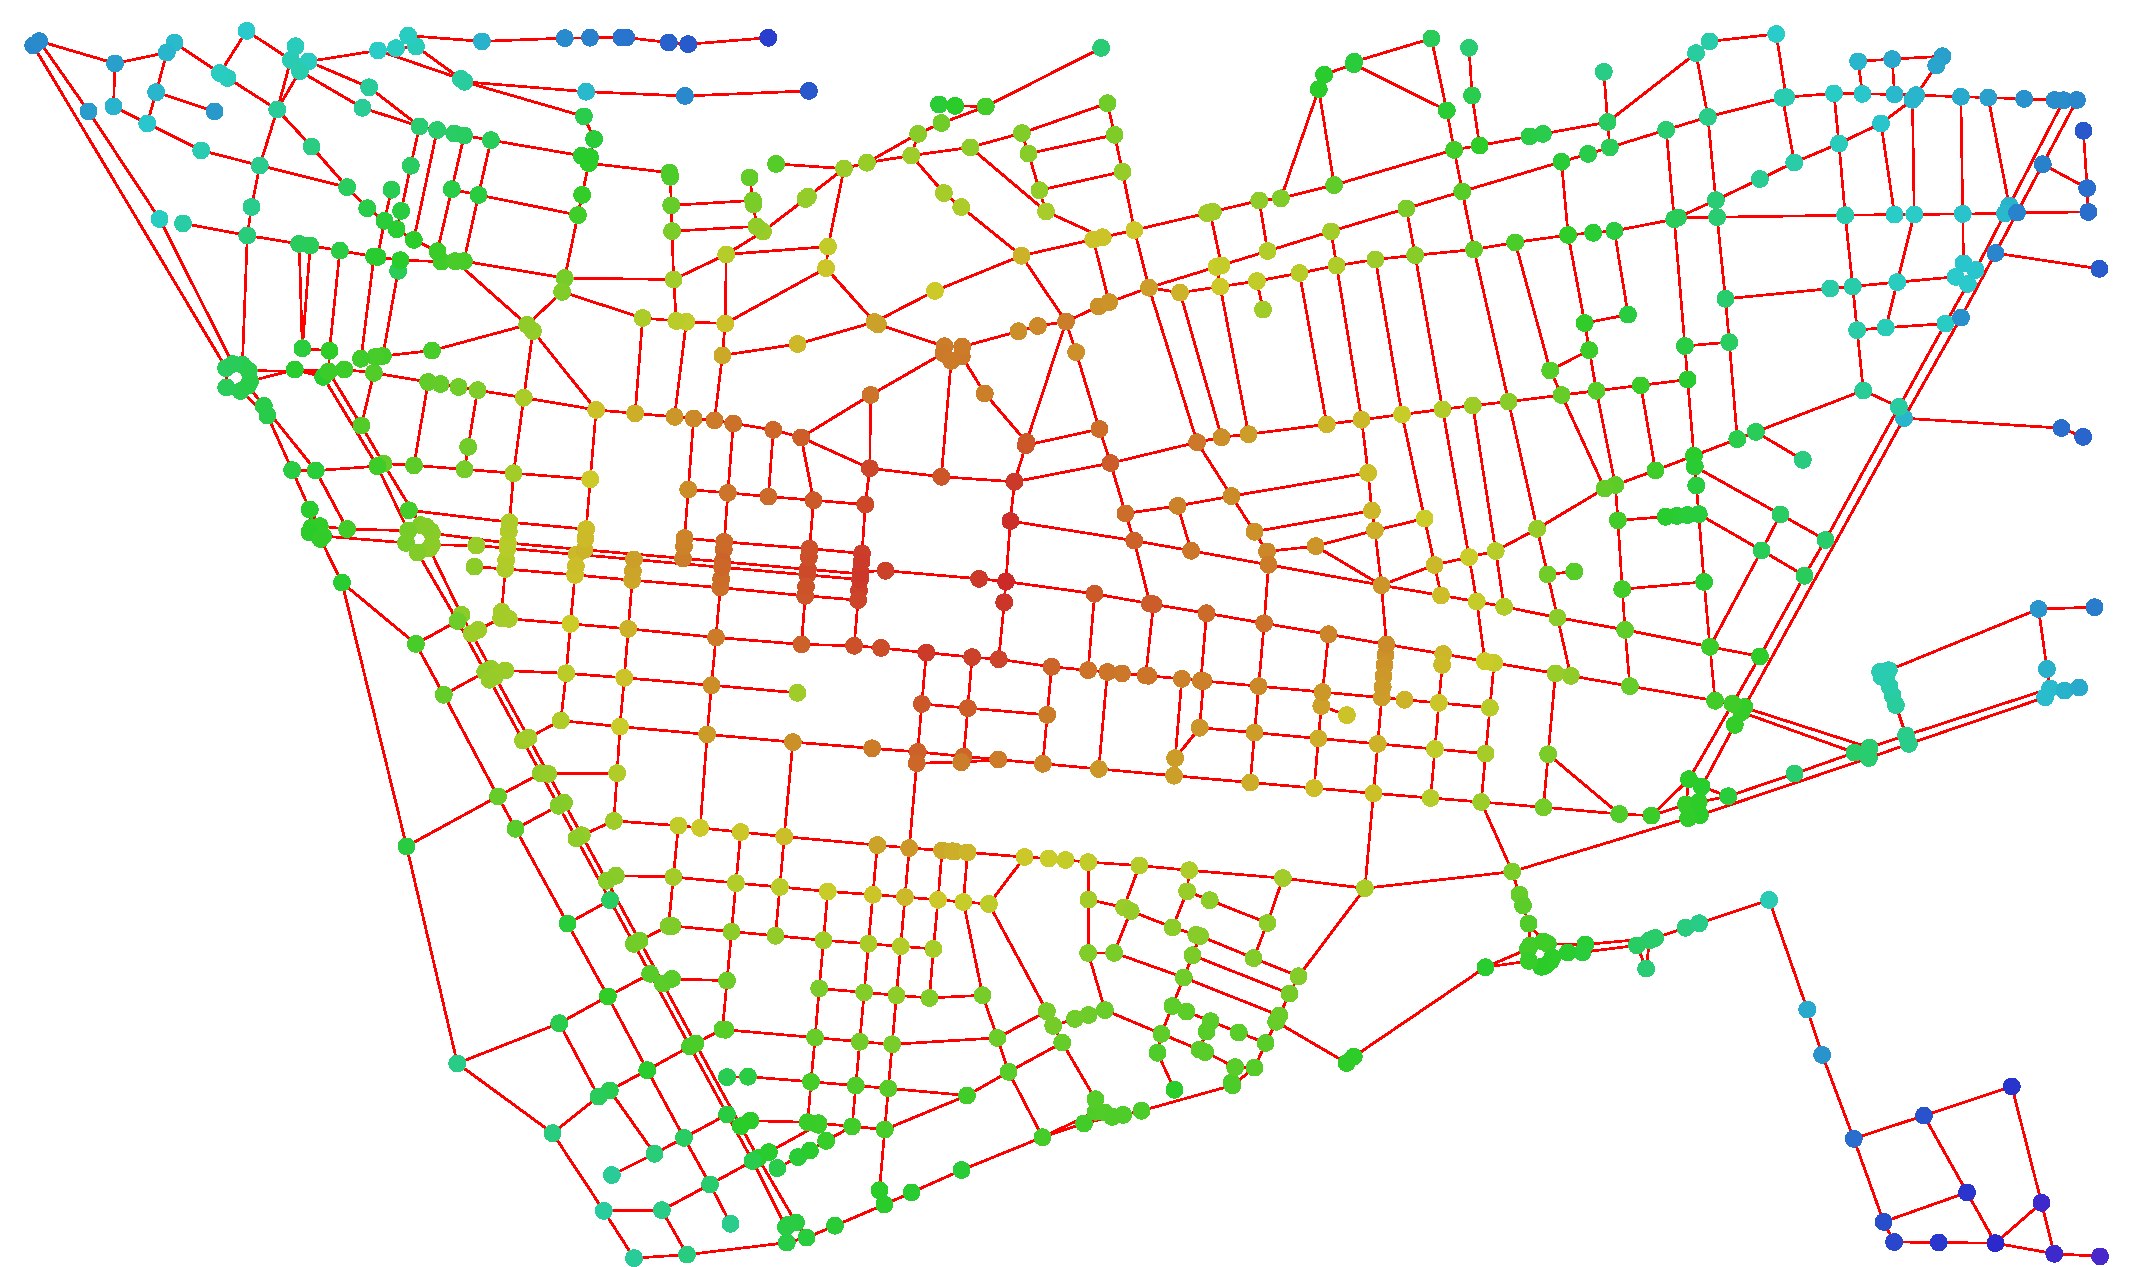
\includegraphics[width=0.49\linewidth]{./img/closeness_centrality.pdf}
	}
	\hfill
	\subcaptionbox{Centralité d'intermédiarité.}[0.49\linewidth][c]{
		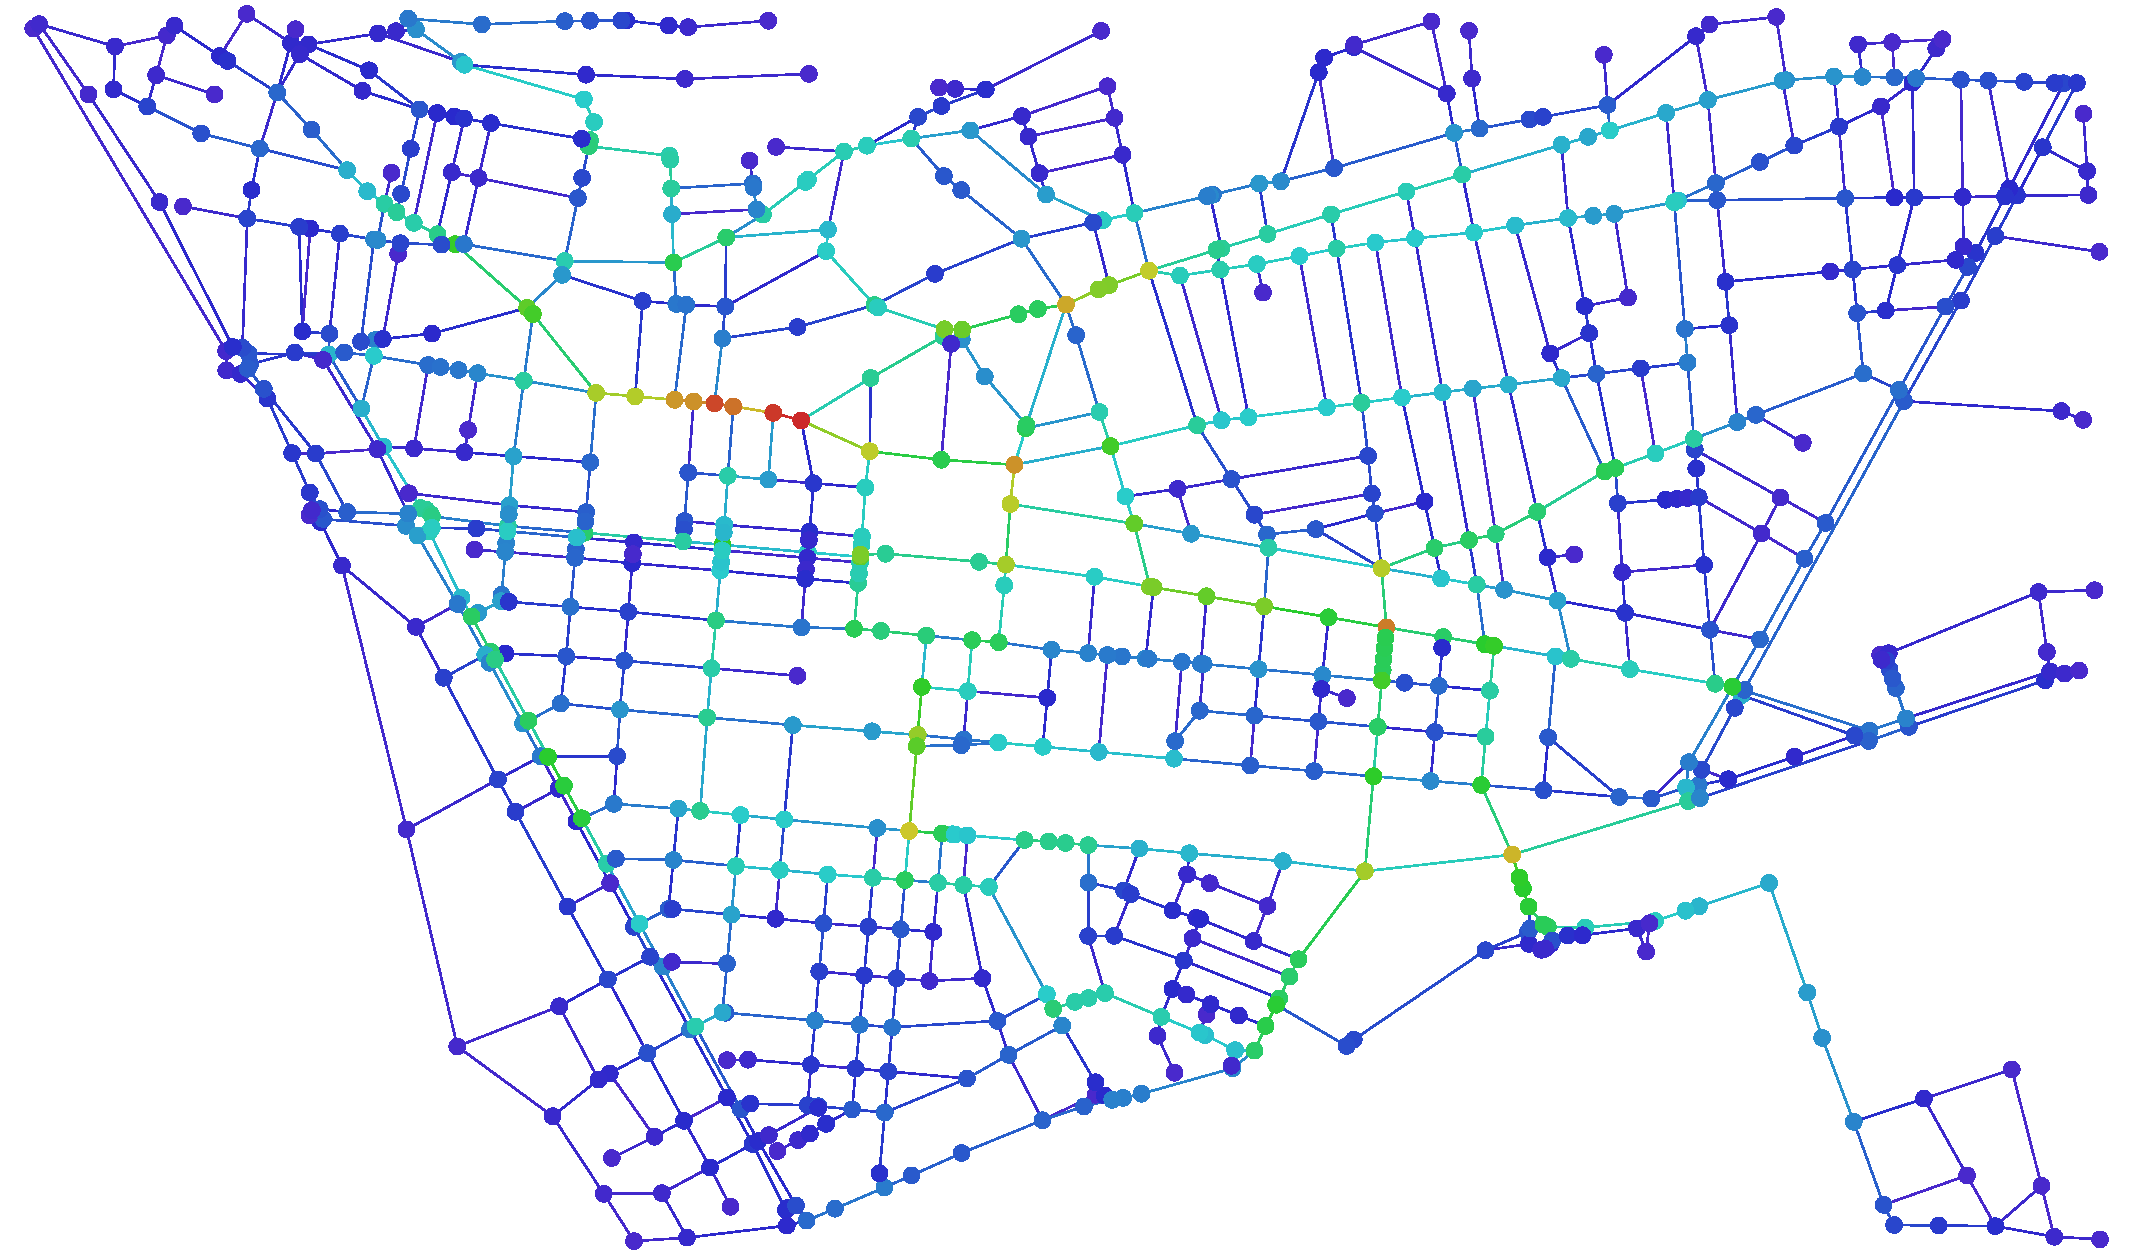
\includegraphics[width=0.49\linewidth]{./img/betwenness_centrality.pdf}
	}
	\caption{Différentes centralités sur le réseau partiel et simplifié de la ville du Havre. Des centralités fortes en rouge aux centralités faibles en bleu.}
	\label{fig:centralities}
\end{figure}

\paragraph{}Dans cette partie nous allons approfondir l'état de l'art de la centralité intermédiaire. Nous verrons donc au début de ce chapitre l'approche classique et les méthodes de calcul, puis nous étudierons les variantes et les références concernant l'approximation de la mesure.

     \section{L'approche classique}

		\subsection{Les origines et les formules de calcul}
		
%%%%%%%%%%%%%%%%%%%%%%%%%
% 
% Les débuts
% 
%%%%%%%%%%%%%%%%%%%%%%%%%

\paragraph{}En 1948, Bavelas \cite{Bavelas1948Mathematical} introduit l'idée qu'un n\oe ud possède une importance accrue lorsqu'il agit comme intermédiaire entre deux autres n\oe uds pour établir une communication. Cette idée est par la suite reprise par plusieurs personnes dont Anthonisse en 1971 \cite{Anthonisse1971Rush}. Il faudra pourtant attendre 1977 et les travaux de Freeman \cite{Freeman1977SetMeasure, Freeman1979Centrality} pour que la centralité intermédiaire se précise et prenne un formalisme clair afin d'être popularisée.


%%%%%%%%%%%%%%%%%%%%%%%%%
% 
% Définition principale
% 
%%%%%%%%%%%%%%%%%%%%%%%%%

\paragraph{}Selon Freeman, la centralité intermédiaire revient à compter le nombre de plus courts chemins passant à travers un n\oe ud parmi tout les plus courts chemins du graphe. Dans un graphe non valué, nous caractérisons la longueur d'un chemin par le nombre d'arêtes qui le constitue.

Soit :

\begin{itemize}
	\item $G=(V, E)$ un graphe orienté (ou non) et non valué tel que $V$ est l'ensemble de ses sommets, et $E$ est l'ensemble de ses arcs. Nous posons également $n=|V|$ et $m=|E|$. 
	\item $C_{B}(k)$ est la centralité associée au n\oe ud $k$.
	\item $g_{st}$ est le nombre de plus court chemin entre $s$ et $t$.
	\item $g_{st}(k)$ est le nombre de plus court chemin entre $s$ et $t$ passant par $k$.
	\item Et nous posons $b_{st}(k)=\frac{g_{st}(k)}{g_{st}}$.
	
	S'il n'existe pas de chemin entre $s$ et $t$, alors $b_{st}(k)=0$.
\end{itemize}

Ainsi la centralité intermédiaire se mesure par :

$$
C_{B}(k)=\underset{s\neq t\neq k}{\sum_s^{n}\sum_t^{n}}b_{st}(k)
$$


%%%%%%%%%%%%%%%%%%%%%%%%%
% 
% Pourquoi les extrémités ne sont pas prises en compte
% 
%%%%%%%%%%%%%%%%%%%%%%%%%

\paragraph{}Nous remarquons que les extrémités des plus courts chemins ne sont pas prises en compte car nous avons : $s\neq t\neq k$. Pourtant, dans la littérature nous pouvons rencontrer des cas où il n'est pas nécessaire de s'embarrasser de cette différence, comme le dit Newman dans \cite{Newman2010Networks}. Effectivement, dans un graphe connexe, le classement des n\oe uds selon leur centralité ne variera pas si nous considérons ou non les extrémités. Et si le graphe possède plusieurs composantes connexes, ce classement ne variera pas non plus au sein des composantes. Toutefois, il est possible que l'ordre global change en fonction de la taille des composantes.

Comme il est plus courant d'utiliser la forme classique avec $s\neq t\neq k$, nous étudierons ce cas de figure. Les modifications à apporter sont, de toute manière, minimes.


%%%%%%%%%%%%%%%%%%%%%%%%%
% 
% Comment normaliser la centralité
% 
%%%%%%%%%%%%%%%%%%%%%%%%%

\paragraph{Normalisation}Freeman propose une manière de comparer la centralité de deux n\oe uds n'étant pas dans un même graphe. Il normalise la centralité de cette manière :
$$
C_{\mathit{NB}}(k)=\frac{2C_B(k)}{n^2-3n+2}
$$

Il considère ainsi que la centralité maximale est atteinte par le n\oe ud central d'un graphe en étoile.

Nous pouvons également normaliser la centralité en la divisant par la centralité maximale trouvée dans le graphe. Nous avons donc :
$$
C_{\mathit{NB}}(k)=\frac{C_B(k)}{\displaystyle \max_{u\leqslant n}(C_B(u))}
$$


%%%%%%%%%%%%%%%%%%%%%%%%%
% 
% Les graphes valués
% 
%%%%%%%%%%%%%%%%%%%%%%%%%

\paragraph{}Le cas des graphes valués ne change pas énormément. Il ne s'agit pas de modifier la mesure en fonction des pondérations (bien que ce soit possible comme nous le verrons plus tard), mais simplement de caractériser les chemins différemment. Nous n'additionnons plus le nombre d'arêtes pour déterminer la longueur d'un chemin mais nous additionnons leur pondération.


		\subsection{L'algorithme de Brandes}

%%%%%%%%%%%%%%%%%%%%%%%%%
% 
% Algorithme de Brandes
% 
%%%%%%%%%%%%%%%%%%%%%%%%%
\paragraph{}La centralité intermédiaire est une mesure très coûteuse à calculer. Effectivement, si nous considérons un algorithme naïf reprenant la formule brute de la centralité intermédiaire, sa complexité en temps est de $O(n^3)$. C'est donc dans l'optique d'améliorer l'algorithme que Brandes en a proposé un autre en 2001, plus rapide, et dont la complexité est de $O(nm)$ pour les graphes non valués, et $O(nm+n^2\log n)$ pour les graphes valués (\cite{Brandes2001Faster}).

\paragraph{}Son algorithme se base sur une formule de récursion. Si nous posons les termes suivants :
\begin{itemize}
    \item $\sigma (s, t)$ : le nombre de plus courts chemins entre $s$ et $t$.
    \item $\sigma (s, t | v)$ : le nombre de plus courts chemins entre $s$ et $t$ passant par $v$.
    \item et $\delta (s, t | v)=\sigma (s, t | v)/\sigma (s, t)$.
\end{itemize}

Nous obtenons ceci :
$$
\delta(s|v) =\sum_{t\in V}\delta(s, t | v)
$$

Ce qui nous permet d'exploiter la relation qui suit :
$$
\delta(s|v)=\sum_{w:\substack{w \in V\\(v, w)\in E \text{ et }\\dist(s, w)=dist(s, v)+1}}\frac{\sigma(s, v)}{\sigma(s, w)}\cdot(1+ \delta(s, w))
$$

Et comme $C_B(v)$ peut s'exprimer ainsi : $C_B(v)=\sum_{s\in V}\delta(s|v)$, il est possible de mesurer la centralité d'un n\oe ud en accumulant les $\delta(s|v)$ progressivement calculés.

\begin{algo}
Entrée :
	un graphe orienté $G=(V, E)$
Données:
	une queue $Q$ initialisée à vide,
	une pile $S$ initialisée à vide,
	Pour chaque $v\in V$
		$\text{dist}[v]$ : la distance depuis la source
		$\text{Pred}[v]$ : la liste des prédécesseurs du plus court chemin depuis la source
		$\sigma [v]$ : le nombre de plus court chemin depuis la source jusqu'à $v$
		$\delta [v]$ : la dépendance de la source sur $v$
Sortie :
	La centralité intermédiaire $C_B[v]$ pour chaque $v\in V$ (initialisée à $0$)
Début
	Pour chaque $s\in V$ faire
		//Problème du plus court chemin
			//Initialisation
			Pour chaque $w\in V$ faire $\text{Pred}[v]$ = liste vide
			Pour chaque $t\in V$ faire $\text{dist}[t]$ = $\infty$ et $\sigma [v]$ = $0$
			$\text{dist}[s]$ = $0$
			$\sigma [v]$ = $1$
			Ajouter $s$ à $Q$
			//Construction du chemin
			Tant que $Q$ n'est pas vide faire
				retirer $v$ de $Q$
				empiler $v$ à  $S$
				Pour chaque $w\in V | \exists (v, w)\in E$ faire
					//Découverte du chemin
					Si $\text{dist}[w]=\infty$ alors
						$\text{dist}[w]$ = $\text{dist}[v]+1$
						ajouter $w$ à $Q$
					Fin si
					//Comptage de chemin - l'arc (v, w) est-il dans un plus court chemin?
					Si $\text{dist}[w]=\text{dist}[v]+1$ alors
						$\sigma [w]$ =  $\sigma [w]+\sigma [v]$
						ajouter $v$ à  $\text{Pred}[w]$
					Fin si
				Fin pour chaque
			Fin tant que
		//Accumulation - rétro-propagation des dépendances
			Pour chaque $v\in V$ faire $\delta [v]$ = 0
			Tant que $S$ n'est pas vide faire 
				dépiler $w$ de $S$
				Pour chaque $v\in \text{Pred}[w]$ faire $\sigma [v]$ = $\sigma [v] + \frac{\sigma [v]}{\sigma [w]} \cdot (1+ \sigma [w])$
				Si $w\neq s$ alors $C_B[w]$ = $C_B[W] + \delta [w]$
			Fin tant que
	Fin pour chaque
Fin
\end{algo}

\paragraph{}Cet algorithme est l'un des plus utilisés aujourd'hui pour effectuer le calcul exact de la centralité intermédiaire. Toutefois, sa complexité reste encore trop importante pour qu'il soit efficace dans de très grands graphes. C'est ainsi que plusieurs auteurs ont proposé des variantes de la mesure afin d'approximer l'ordre d'importance des n\oe uds (\cite{Brandes2007Centrality}), tandis que d'autres ont modifié l'approche classique lorsque celle-ci ne permettait pas de mettre en valeur certains n\oe uds importants (\cite{Newman2005MeasureBetweenness}). Nous allons donc approfondir dans la section qui suit ces différentes variantes.

     \section{Les variantes et les approximations}

		\subsection{Les variantes}

\paragraph{}L'un des défauts de la centralité intermédiaire est que l'information transite au sein du graphe en empruntant les plus courts chemins. Pourtant, nous nous rendons rapidement compte que ce n'est pas toujours le cas. Effectivement, dans certains réseaux, notamment les réseaux sociaux, les entités associées aux n\oe uds ont une connaissance imparfaite de la topologie du graphe. Elles ne sont donc pas en mesure de "router" les messages efficacement en leur faisant emprunter exclusivement les plus courts chemins.

\paragraph{}Ainsi, en 1991, Freeman \textit{et al.} proposent un nouveau modèle basé sur les flots \cite{FreemanBorgattiWhite1991Centrality}. Il ne s'agit donc plus de calculer les plus courts chemins mais de considérer l'ensemble des n\oe uds appartenant au flot maximal. Ce dernier est défini selon l'algorithme de Ford et Fulkerson \cite{Ford1956Maximal}.

\paragraph{}Ces idées ont ensuite été reprises, notamment par Borgatti \cite{Borgatti2005Centrality}. Dans son article, il montre qu'il faut parfois considérer un processus particulier pour calculer le flot. Ceci implique que le modèle de Freeman n'est pas toujours approprié et qu'il est nécessaire de l'adapter.

\paragraph{}La centralité basée sur les flots a l'avantage de fournir une liste de n\oe uds potentiellement plus importante. Et celle-ci peut contenir les n\oe uds appartenant au plus court chemin ou à de "bon" chemin. Cependant, cette propriété n'est pas toujours vérifiée. Le flot maximal entre deux sommets d'un graphe peut tout à fait emprunter un détour important, bien loin du plus court chemin ou des "bons" chemins. 

\paragraph{}De plus, l'algorithme de Ford et Fulkerson ne considère plus de nouveaux n\oe uds, ou chemins, lorsque nous avons atteint le flot maximal sur la coupe minimale. Par exemple sur la figure \ref{fig:flot_max}, la recherche de flot détermine qu'il est maximal entre les sommets de couleur en empruntant le chemin vert, et l'arête valuée à 1 appartient à la coupe minimale. L'algorithme stoppera donc son calcul pour le flot entre ces sommets alors que le chemin orange semble tout aussi intéressant. 

\begin{figure}[h!]
	\centering
	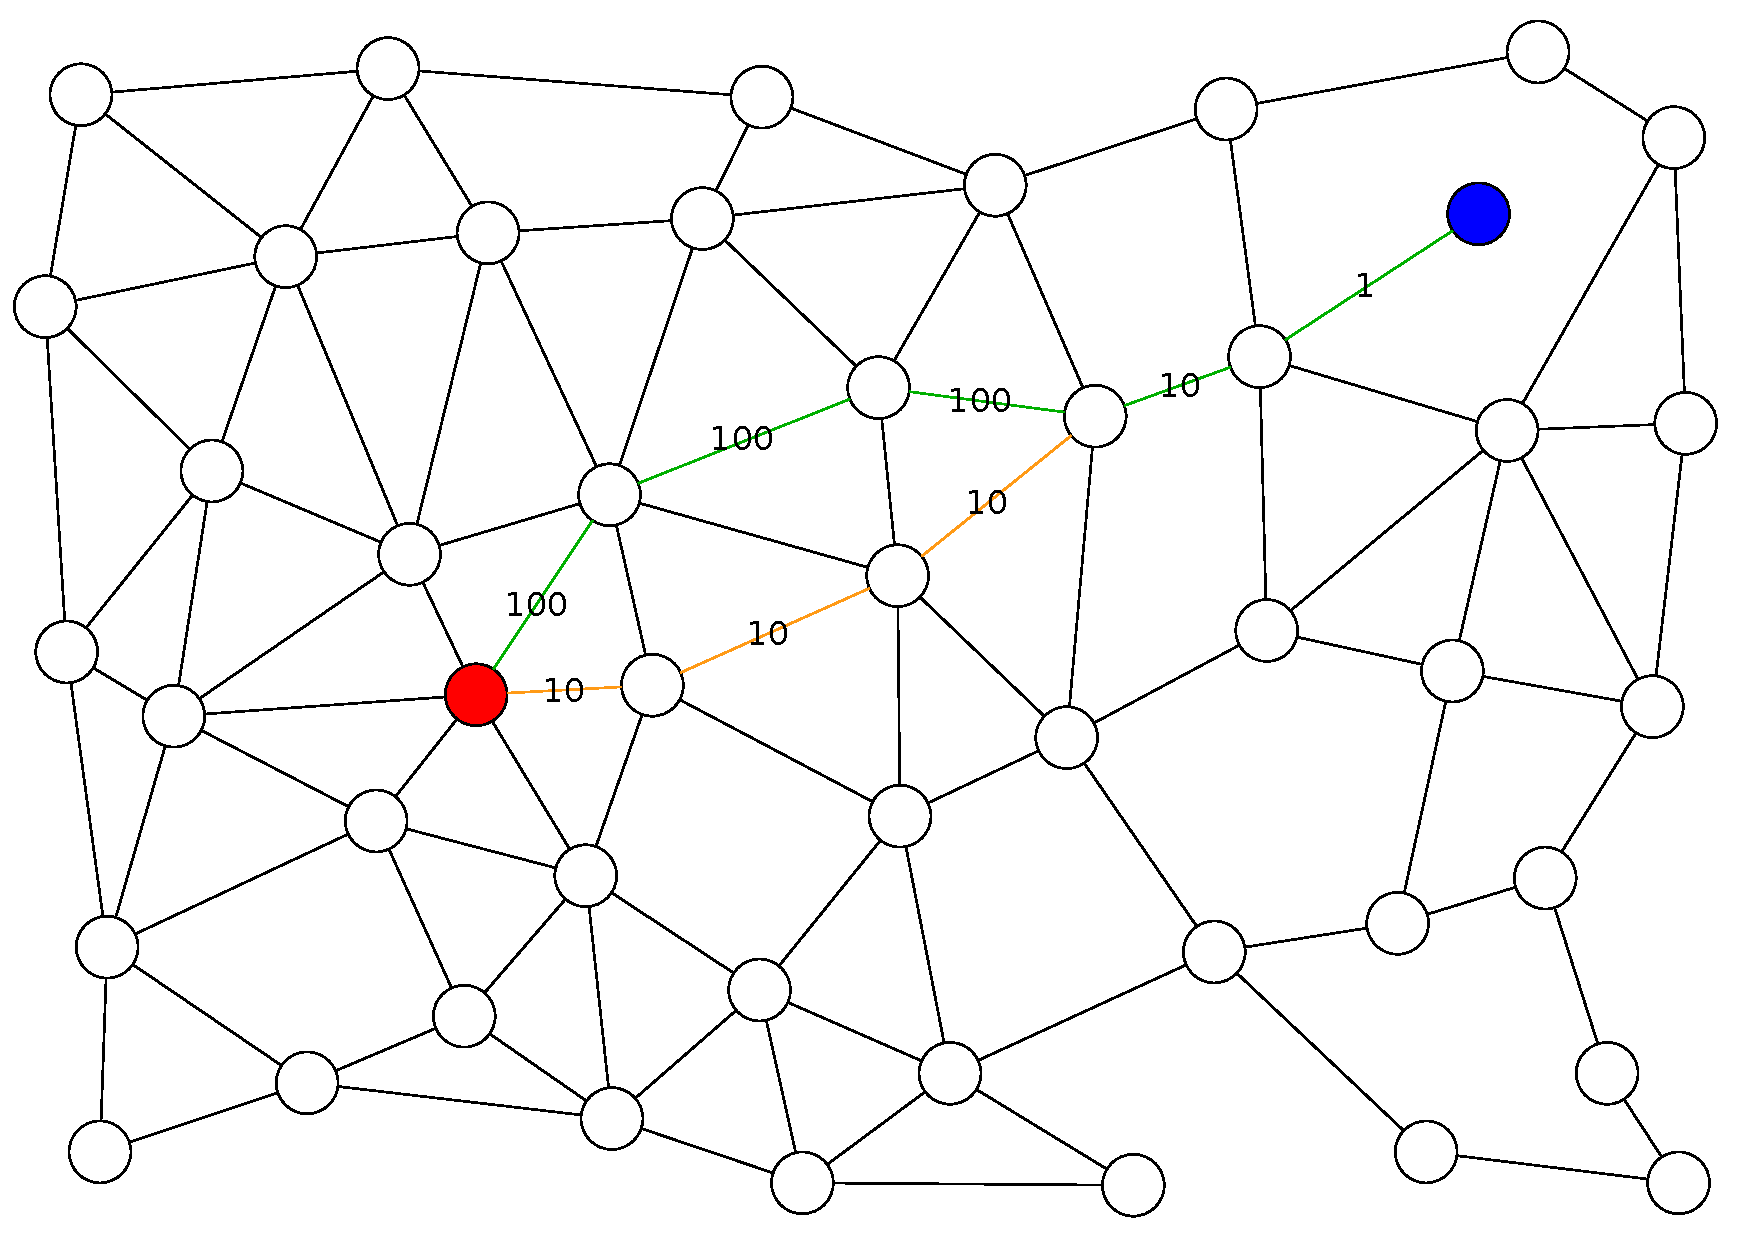
\includegraphics[width=1.\textwidth]{./img/probleme_centrality_flow.pdf}
	\caption{Mise en valeur du flot maximal (en vert) entre deux sommets et d'une portion d'un chemin alternatif (en orange). Les valeurs correspondent à une capacité de flot.}
	\label{fig:flot_max}
\end{figure}

\paragraph{}Nous remarquons aussi que dans un réseau routier il n'est pas nécessaire d'atteindre la limite du volume d'une route avant que certains véhicules décident d'emprunter d'autres chemins. Nous pouvons ainsi voir que ce modèle n'est pas à l'image de la réalité (en tout cas pour notre objet d'étude). Ces remarques sont d'ailleurs mises en valeur dans \cite{Newman2005MeasureBetweenness} et \cite{Gleyze2005Vulneraibilite}.

\paragraph{}D'autres méthodes ont également vu le jour afin de considérer plus de chemins, et pas nécessairement les plus courts. Elles se basent notamment sur la recherche de chemins d'une longueur maximale, comme la k-centralité intermédiaire (k-betweenness centrality) dont parle Borgatti dans \cite{Borgatti2006GraphTheoretic}. Il s'agit de prendre en compte tous les chemins étant d'une longueur k au plus. Cette idée a été formalisée dans \cite{Jiang2009Generalizing} qui en propose une implémentation parallélisée.

À partir de la même idée, il est également possible de considérer les chemins dont les arêtes (ou les n\oe uds) sont disjoints.

%%%%%%%%%%%%%%%%%%%%%%%%%
% 
% Variantes pondérant les contributions en fonction de la longueur
% 
%%%%%%%%%%%%%%%%%%%%%%%%%

\paragraph{}De même, il existe des formules prenant en compte les longueurs des chemins. Celles-ci se montrent souvent intéressantes et fournissent des données supplémentaires à la mesure. Certains auteurs, notamment ceux issus de la sociologie, préconisent de pondérer les plus courts chemins proportionnellement à leur longueur inverse (\cite{Borgatti2006GraphTheoretic}). Ainsi, nous augmenterons la centralité d'un n\oe{}ud jouant le rôle d'intermédiaire dans des chemins de petite taille. 
Soit :
$$
C_{B}(k)=\underset{s\neq t\neq k}{\sum_s^{n}\sum_t^{n}}\frac{1}{\text{dist}(s, t)}b_{st}(k)
$$
tel que $\text{dist}(s, t)$ retourne la longueur du chemin entre $s$ et $t$.

\paragraph{}Dans \cite{Geisberger2008Better} et \cite{Brandes2007OnVariants}, les auteurs montrent que nous pouvons également pondérer la contribution d'un chemin en fonction de la place du n\oe ud dans ce chemin. Geisberger \textit{et al.} s'en servent pour effectuer une approximation de la centralité mais Brandes affirme qu'il peut s'agir d'une variante intéressante de celle-ci. Ainsi le n\oe{}ud peut être mieux pondéré si :
\begin{itemize}
    \item il se trouve au centre, tel que :
$$
C_{B}(k)=\underset{s\neq t\neq k}{\sum_s^{n}\sum_t^{n}}
	\frac{2 \times \text{min}(\text{dist}(s, k), \text{dist}(k, t))}
	     {\text{dist}(s, t)}
	b_{st}(k)
$$
	\item il se trouve proche du n\oe ud source du chemin, tel que :
$$
C_{B}(k)=\underset{s\neq t\neq k}{\sum_s^{n}\sum_t^{n}}\frac{\text{dist}(k, t)}{\text{dist}(s, t)}b_{st}(k)
$$
	\item il se trouve proche du n\oe ud cible du chemin, tel que :
$$
C_{B}(k)=\underset{s\neq t\neq k}{\sum_s^{n}\sum_t^{n}}\frac{\text{dist}(s, k)}{\text{dist}(s, t)}b_{st}(k)
$$
\end{itemize}

\paragraph{}Ces versions de la centralité peuvent notamment prendre de l'importance dans des graphes valués comme un réseau routier. Prenons l'exemple de la figure \ref{fig:centrality_non_symetric_graph}, si nous considérons une approche classique du calcul de la centralité, alors les n\oe uds rouge et orange devraient obtenir le même score. Pourtant, si nous considérons la pondération sur les arcs, il semble bien qu'il existe une différence entre ces deux n\oe uds. En traçant un cercle passant par les n\oe uds vert nous nous apercevons que le n\oe ud rouge en est le centre. Si nous souhaitons faire apparaître ce type d'information dans la mesure finale, alors nous pouvons utiliser la formule ci-dessus favorisant les n\oe uds au centre des chemins.

\begin{figure}[h!]
	\centering
	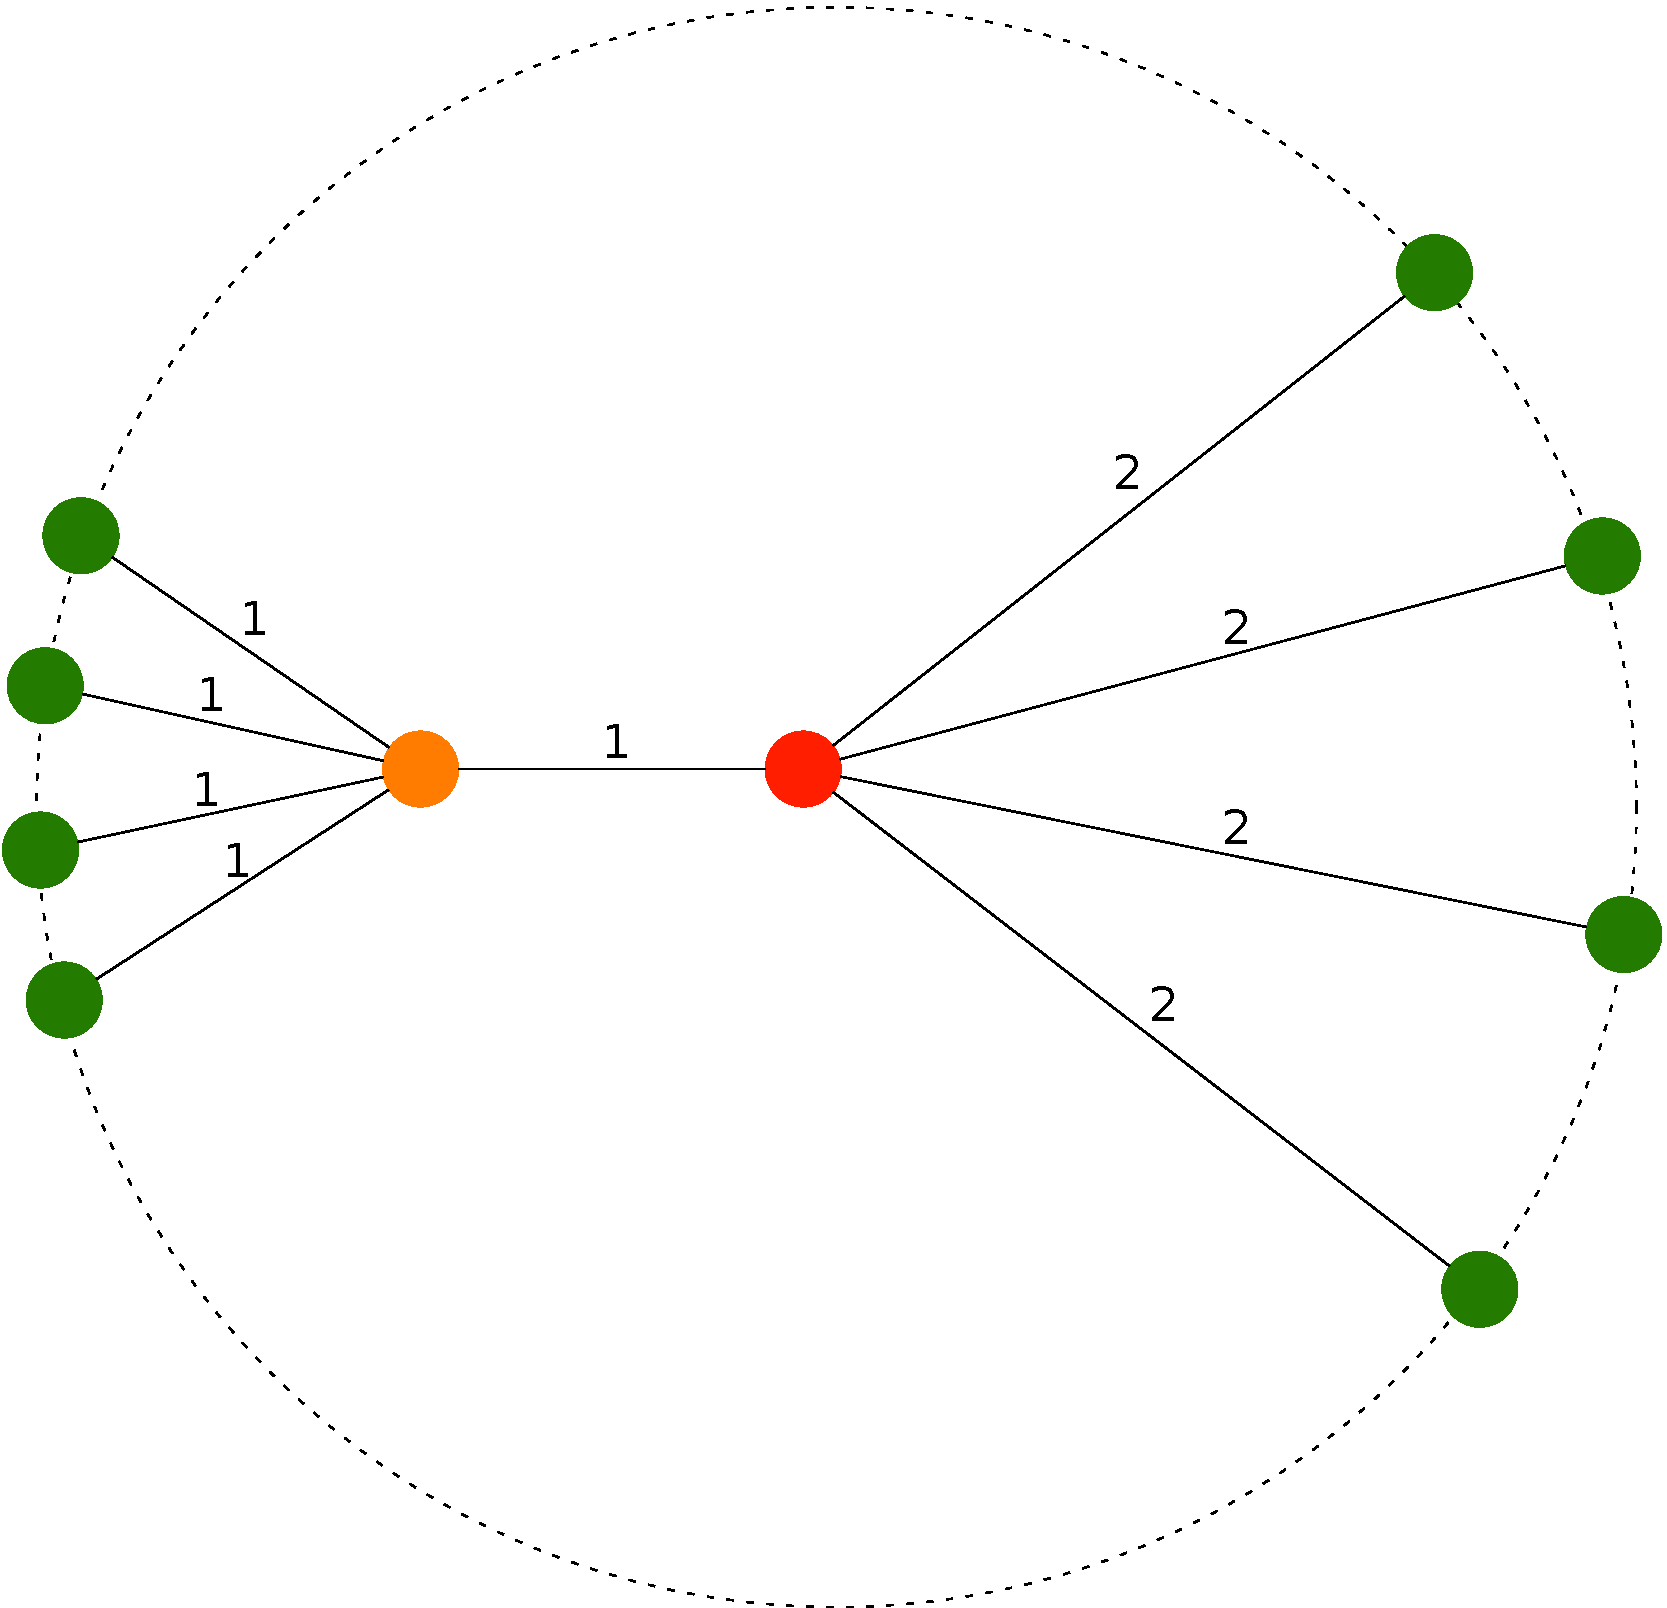
\includegraphics[width=1.\textwidth]{./img/centrality_non_symetric_graph.pdf}
	\caption{Graphe valué dans lequel nous pouvons différencier le n\oe ud rouge de celui orange avec une formule adaptée.}
	\label{fig:centrality_non_symetric_graph}
\end{figure}

\newpage

		\subsection{Les approximations}

\paragraph{}Un autre défaut, que nous avons déjà abordé, est le temps de calcul. Même s'il existe un algorithme résolvant le problème en $O(nm)$, lorsque nous traitons des graphes de plusieurs centaines de milliers ou de millions de n\oe uds, la complexité est encore bien trop grande. Ainsi, dans l'objectif de réduire le coût de calcul, Brandes a traité ce problème dans \cite{Brandes2007Centrality} en reprenant une idée issue de \cite{Eppstein2004Fast}.

\paragraph{}L'idée directrice est d'utiliser un sous ensemble de n\oe uds "pivots". Nous résolvons ensuite les problèmes de plus courts chemins partant de ces sommets vers tous les autres, et grâce à une formule de probabilité, il devient possible d'estimer la valeur réelle de la centralité de chaque n\oe ud.

Brandes montre qu'il est préférable de sélectionner les pivots de façon aléatoire, et que leur nombre dépend de la taille du graphe.

\paragraph{}Geisberger \textit{et al.} proposent une extension de ce modèle dans \cite{Geisberger2008Better}. Effectivement, la version de Brandes tend à favoriser les n\oe uds proches des pivots, ce qui biaise le résultat final. Ils ont donc décidé de retirer ce biais à l'aide d'une méthode qui ajuste ces résultats.

\paragraph{}Alahakoon \textit{et al.} proposent également un modèle estimant la centralité dans \cite{Alahakoon2011KPath}. Les auteurs définissent un algorithme dans lequel nous sélectionnons des n\oe uds pivots à partir desquels nous faisons transiter une information (ou une entité) selon une marche aléatoire, le chemin parcouru ne devant pas dépasser une certaine longueur comprise entre 1 et un paramètre K. Les auteurs de ce papier appuient une partie de leurs travaux sur ceux de Brandes. La principale contribution consiste à se servir d'une marche aléatoire et de limiter la longueur des chemins à une taille maximale.

\paragraph{}Toutefois, il est nécessaire de noter que sa méthode s'applique très bien sur des réseaux sociaux mais il n'est pas garanti d'obtenir des résultats optimaux dans le cas général. Effectivement, les réseaux sociaux ont cette particularité : la contribution apportée à la centralité des n\oe uds par les chemins de grande taille est moins importante que la contribution apportée par les chemins de petite taille \cite{Friedkin1983Horizons, Alahakoon2011KPath}. Il est donc logique d'obtenir des résultats intéressants pour de tels réseaux en bornant la taille des chemins. Mais si nous utilisons un réseau viaire, les n\oe uds à forte centralité peuvent tout à fait faire partie d'axe de grande taille (comme les axes transversaux ou les points d'articulation).

\paragraph{}L'utilisation d'une marche aléatoire pour calculer la centralité a quant à elle été proposée par Newman dans \cite{Newman2005MeasureBetweenness}. Toutefois, avant de présenter directement et plus en détail ce concept, nous allons expliquer les méthodes d'analyses que nous avons employées pour comparer les mesures développées et l'approche classique.


\chapter{Les méthodes d'analyses}

	\section{Les méthodes de comparaison}
	
\paragraph{}Nos hypothèses initiales se basaient sur nos impressions de similarités des colorations des graphes. Nous ne pouvions donc nous contenter de cette approche pour juger des résultats.

\paragraph{}Dans un premier temps nous nous sommes intéressés aux coefficients de corrélation de Pearson et de Spearman. Il s'agit de mesures utilisées en statistiques. Elles fournissent une valeur entre -1 et 1 indiquant la dépendance qui existe ou non entre deux variables statistiques. Plus la valeur absolue de la mesure est proche de 1, plus les deux variables sont corrélées. Au contraire,  plus la valeur est proche de zéro, moins les variables sont corrélées. La mesure de Pearson permet de détecter une corrélation linéaire, tandis que celle de Spearman met en valeur une corrélation non linéaire.

\paragraph{}Si nous avons deux échantillons associés aux variables $X$ et $Y$, alors le coefficient de Pearson se calcule ainsi : 
$$
r_{xy}=
\frac{\sum\limits_{i=1}^n (x_i-\bar{x})(y_i-\bar{y})}{\sqrt{\sum\limits_{i=1}^n (x_i-\bar{x})^2 \sum\limits_{i=1}^n (y_i-\bar{y})^2}}
$$
tel que : $x_i$ (resp. $y_i$) est la i\up{ème} valeur de $X$ (resp. $Y$) et $\bar{x_i}$ (resp. $\bar{y_i}$) est la moyenne des valeurs de l'échantillon de $X$ (resp. $Y$).
 
\paragraph{}Le coefficient de Spearman se calcule de la même manière mais plutôt que de considérer directement la valeur de chaque $x_i$ et $y_i$, nous considérons le rang que possède ces variables dans une liste ordonnée.

\paragraph{}Nous avons également décidé de compléter notre panel de méthodes avec une approche plus graphique. Nous construisons la liste ordonnée des n\oe uds selon l'une des deux mesures que nous souhaitons comparer. Puis nous traçons sur un graphique la courbe représentant ce classement avec en abscisses l'identifiant des n\oe uds et en ordonnées la mesure de chacun d'entre eux. Enfin, nous positionnons sur le même graphique et pour chaque n\oe ud, le score obtenu par la deuxième mesure. Si le deuxième tracé représente une courbe, alors nous pouvons affirmer que les deux mesures sont corrélées directement, et la finesse de cette courbe montrera le degré de corrélation.

\paragraph{}Cette deuxième méthode permet de confirmer la corrélation indiquée par les coefficients, car parfois nous obtenons des coefficients à 0.6 ou 0.7 alors que la corrélation n'est pas du tout significative. L'interprétation des coefficients est donc délicate dans certains cas. Les graphiques permettent ainsi cette interprétation.

	\section{Les graphes utilisés}
	
\paragraph{}Afin de déterminer si nos modèles fournissaient des résultats corrects dans le cas général, nous les avons confrontés à plusieurs types de graphes différents. Nous avons donc utilisé d'un côté les générateurs de graphes présents dans la librairie GraphStream et de l'autre des représentations des réseaux viaires de la ville du Havre et de celle de Rouen.

\paragraph{Le générateur de "small-world"}
Ce premier type de graphe est basé sur le modèle de Watts et Strogatz présent dans \cite{Watts1998Collective}. Il s'agit de créer une structure en anneau dont les n\oe uds ont $k$ voisin(s). Puis nous modifions aléatoirement certaines arêtes afin qu'une de leurs extrémités soit connectée à un autre n\oe ud choisi aléatoirement selon une probabilité $\beta$ (voir figure \ref{fig:screenshot_small_world}).

\begin{figure}[h!]
	\centering
	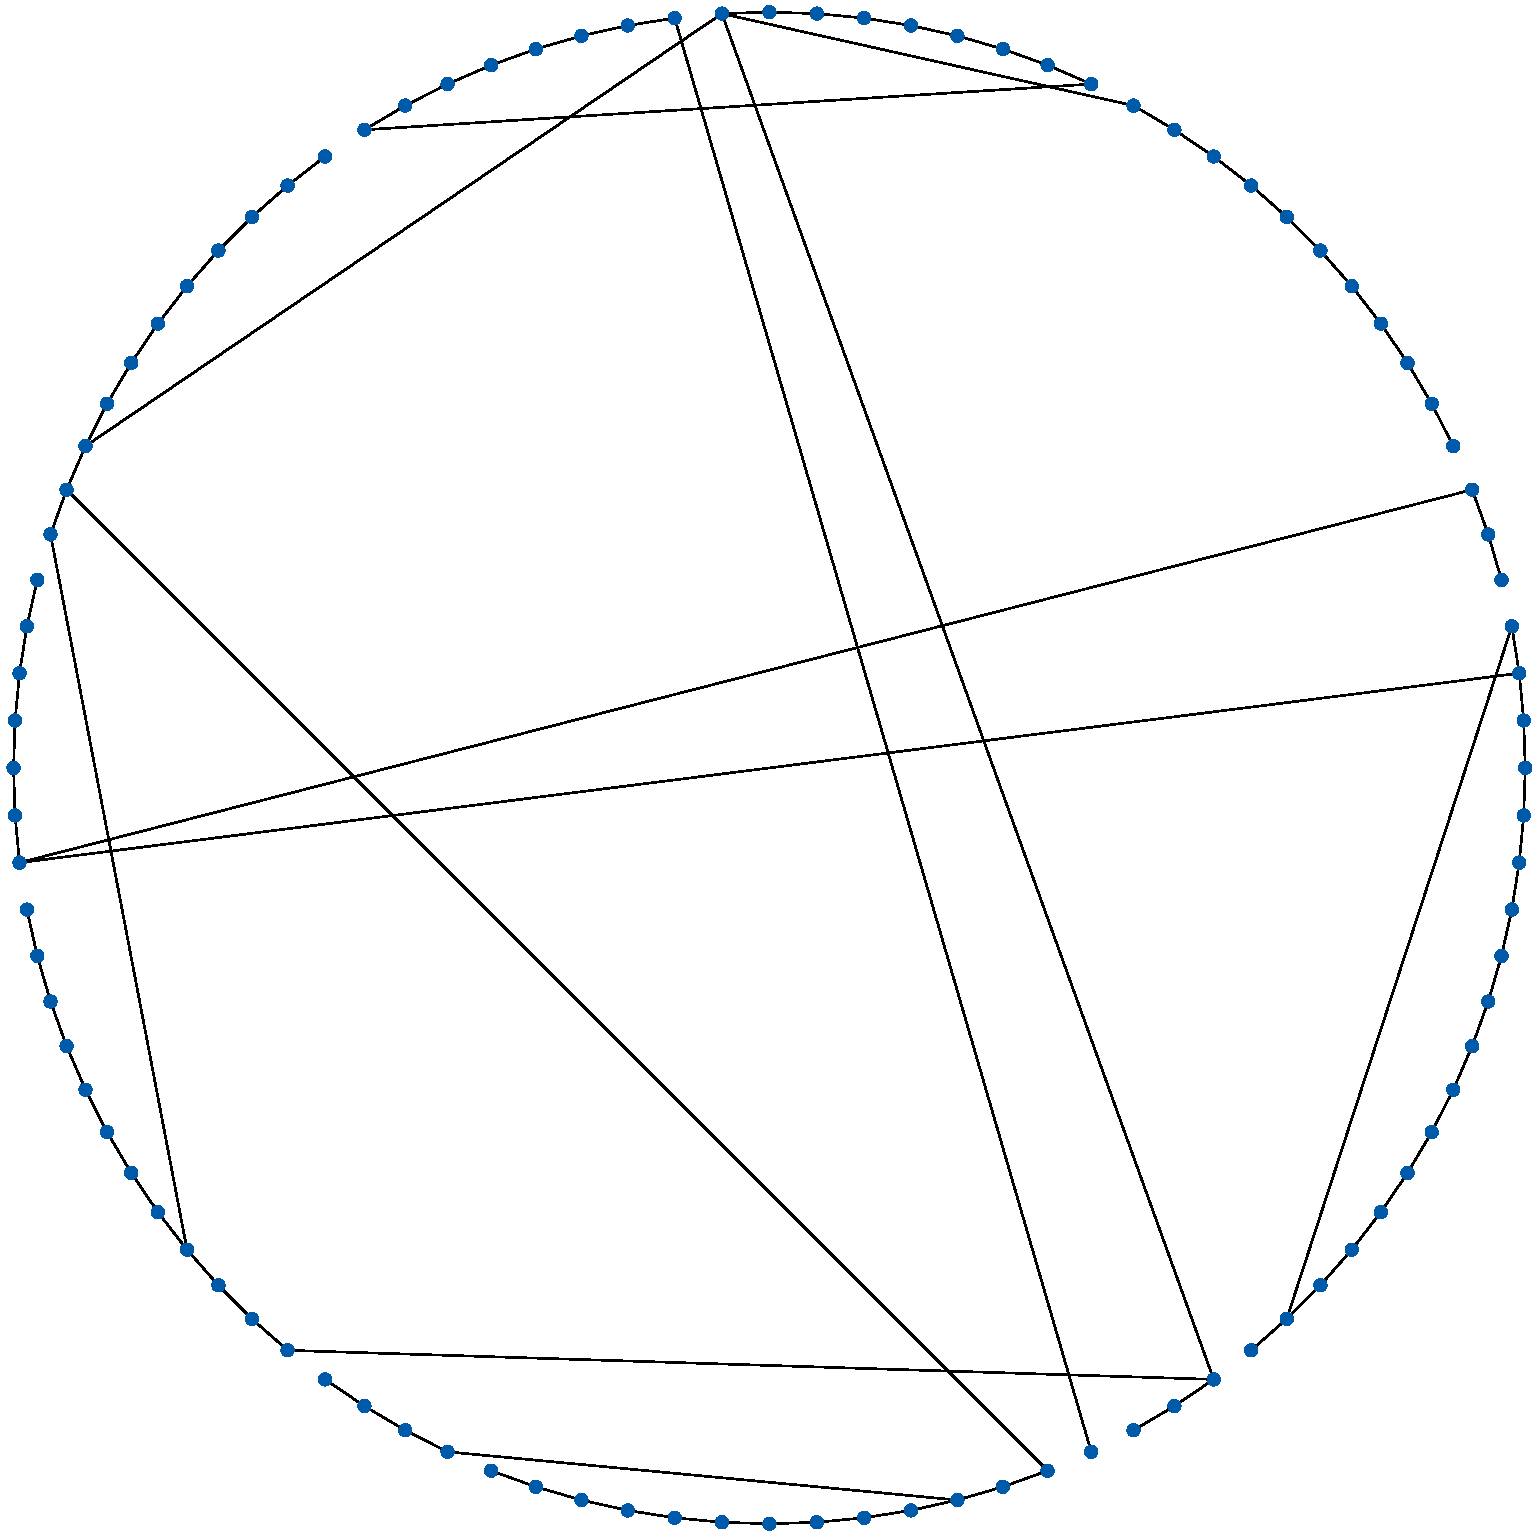
\includegraphics[width=0.5\textwidth]{./img/screenshot_small_world.pdf}
	\caption{Représentation d'un small-world avec 100 n\oe uds, $k=2$ voisins et $\beta=0.1$.}
	\label{fig:screenshot_small_world}
\end{figure}

\paragraph{Le générateur de grille}Nous avons également utilisé un générateur de grille car il s'agit d'une topologie très régulière et assez simple mais qui peut poser certains problèmes. Effectivement, entre deux n\oe uds quelconques d'une grille, il existe plusieurs plus courts chemins. Et la centralité classique prend en compte chacun de ces chemins. Pourtant, nous verrons par la suite que nos méthodes ne définissent qu'un seul chemin entre les paires de n\oe uds. Il fallait donc vérifier si nous pouvions tout de même obtenir des résultats cohérents dans ce cas de figure.

\paragraph{Le générateur d'attachement préférentiel}
Celui-ci s'appuie sur le modèle de Barabàsi et d'Albert proposé dans \cite{Barabasi1999Emergence}. À chaque étape nous générons un n\oe ud qui sera relié par une ou plusieurs arête(s) à un ou plusieurs n\oe uds choisi(s) selon une sélection aléatoire biaisée par son degré (voir figure \ref{fig:sceenshot_preferential_attachement}).

\begin{figure}[h!]
	\centering
	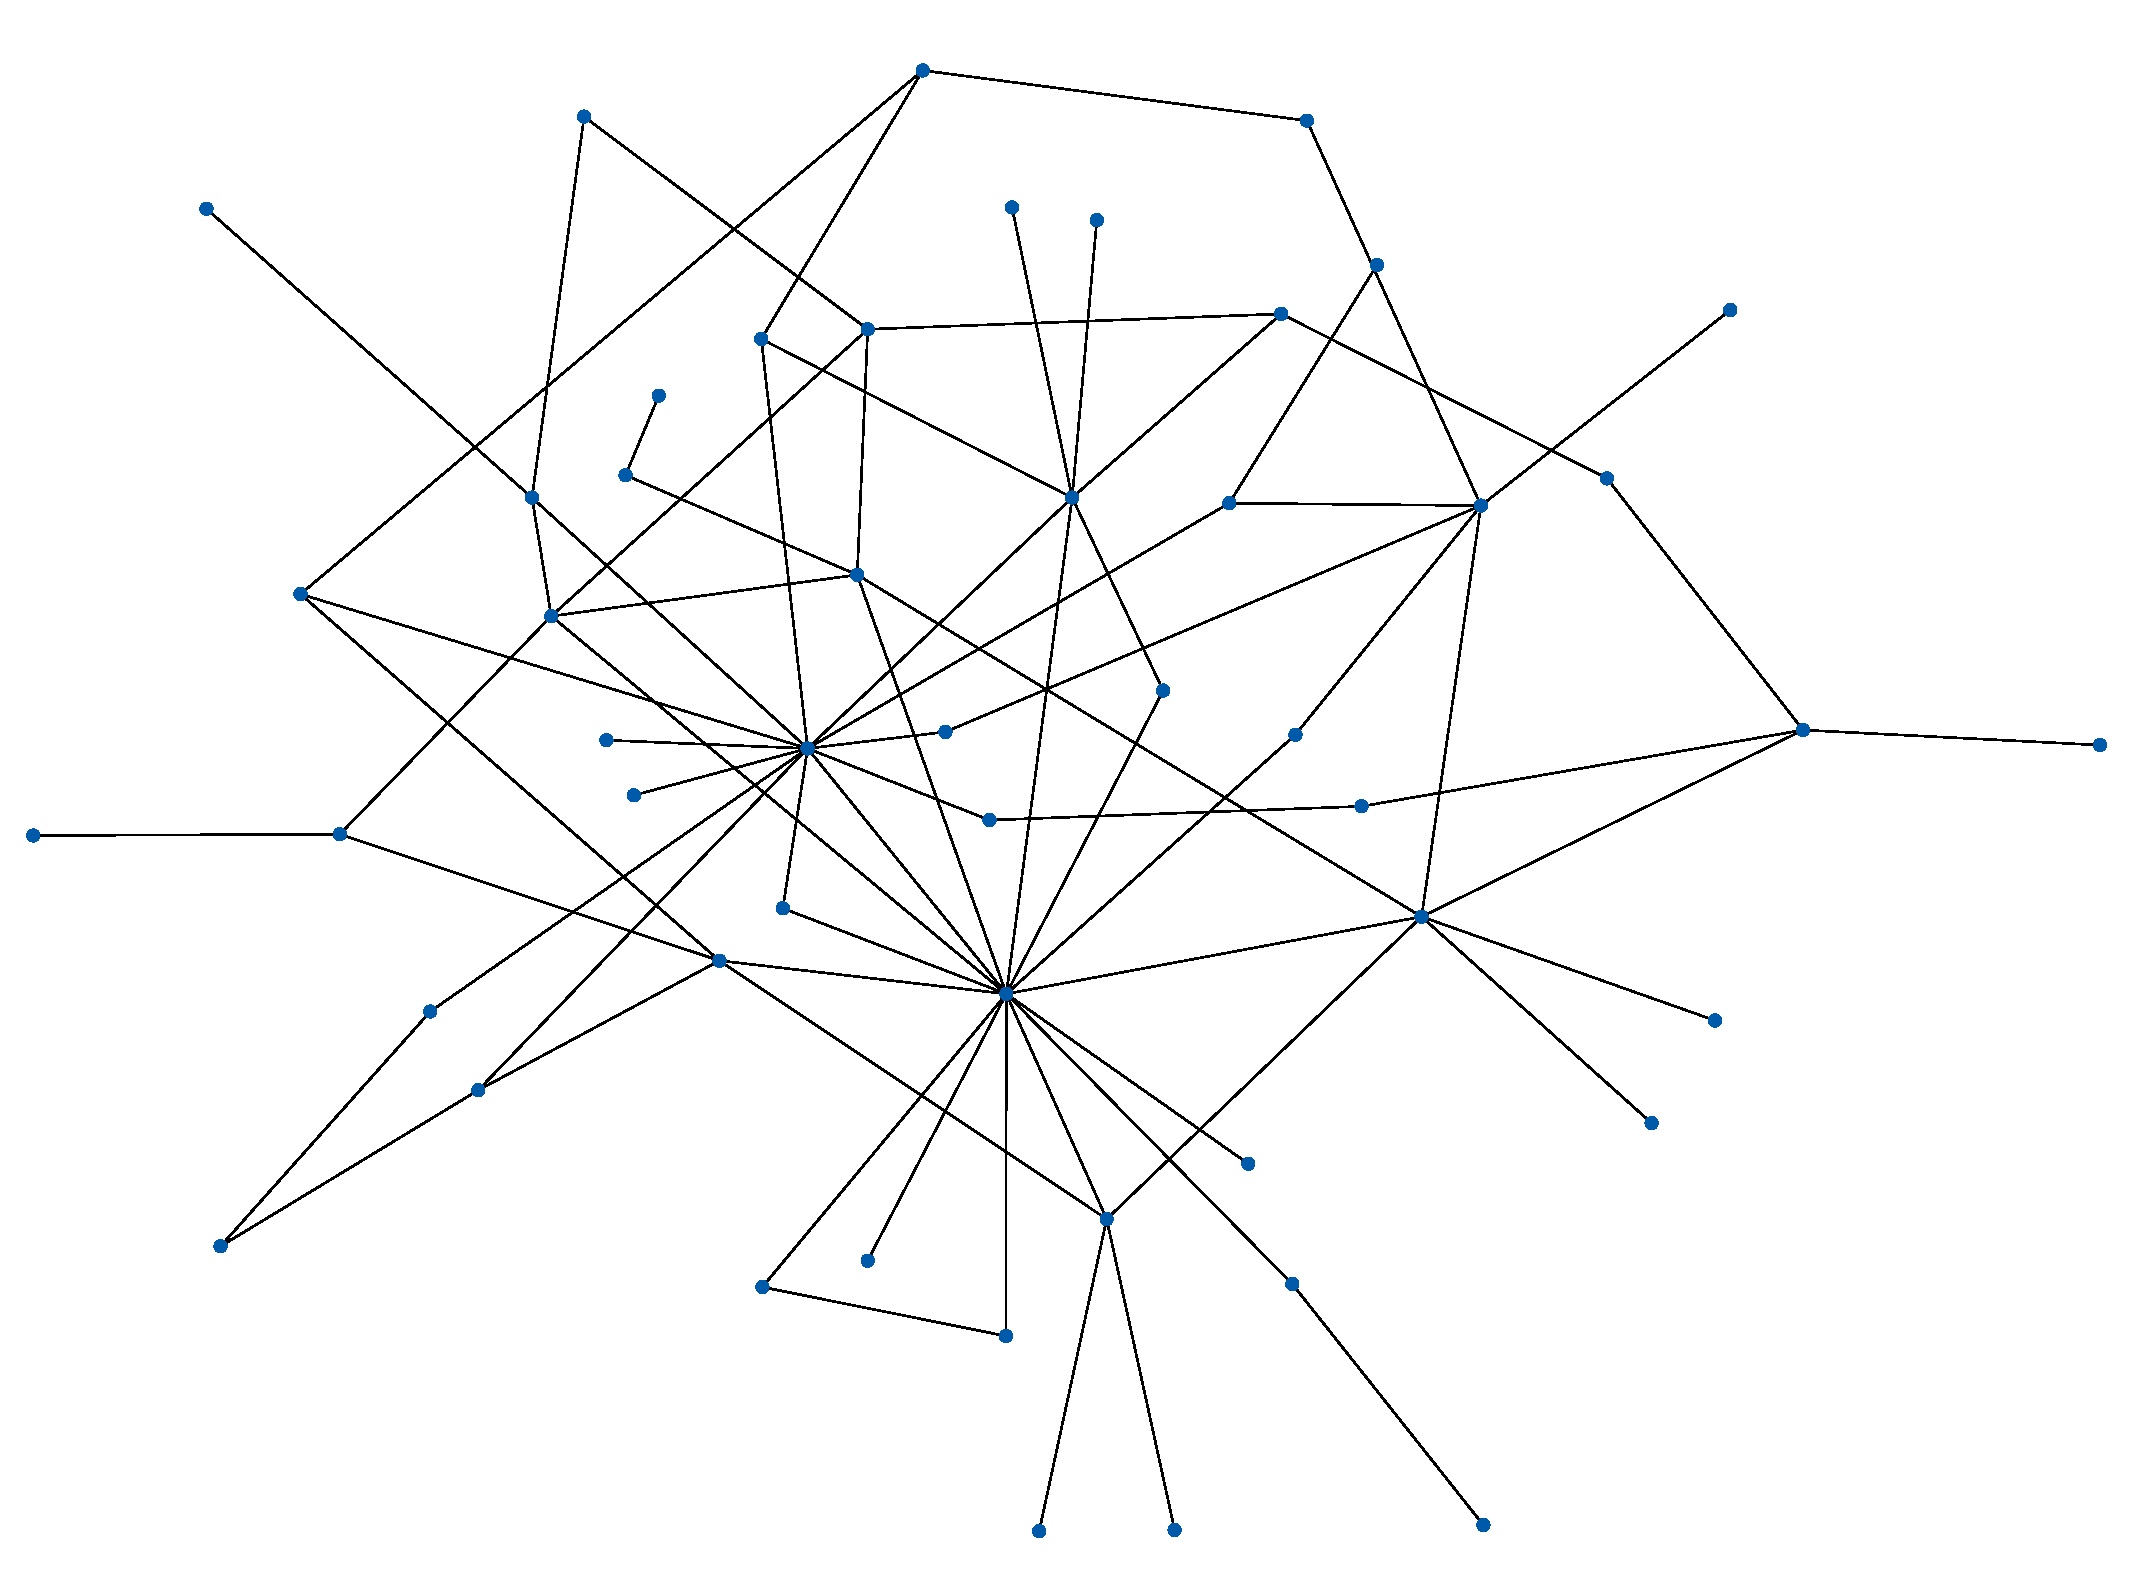
\includegraphics[width=1.\textwidth]{./img/sceenshot_preferential_attachement.pdf}
	\caption{Représentation d'un attachement préférentiel avec 50 n\oe uds, et 2 arêtes au maximum créées par tour.}
	\label{fig:sceenshot_preferential_attachement}
\end{figure}

\paragraph{Le générateur de graphe de Dorogovtsev-Mendes}Il s'agit de l'algorithme proposé par Dorogovtsev et Mendes dans \cite{Dorogovtsev2002evolution} qui crée des graphes planaires dont la distribution des degrés suit une loi de puissance. À l'initialisation, nous créons trois n\oe uds et trois arêtes disposés en triangle. Puis à chaque tour, nous ajoutons un nouveau n\oe ud que nous connectons aux extrémités d'une arête choisie aléatoirement (voir figure \ref{fig:screenshot_Dorogovtsev_Mendes}).

\begin{figure}[h!]
	\centering
	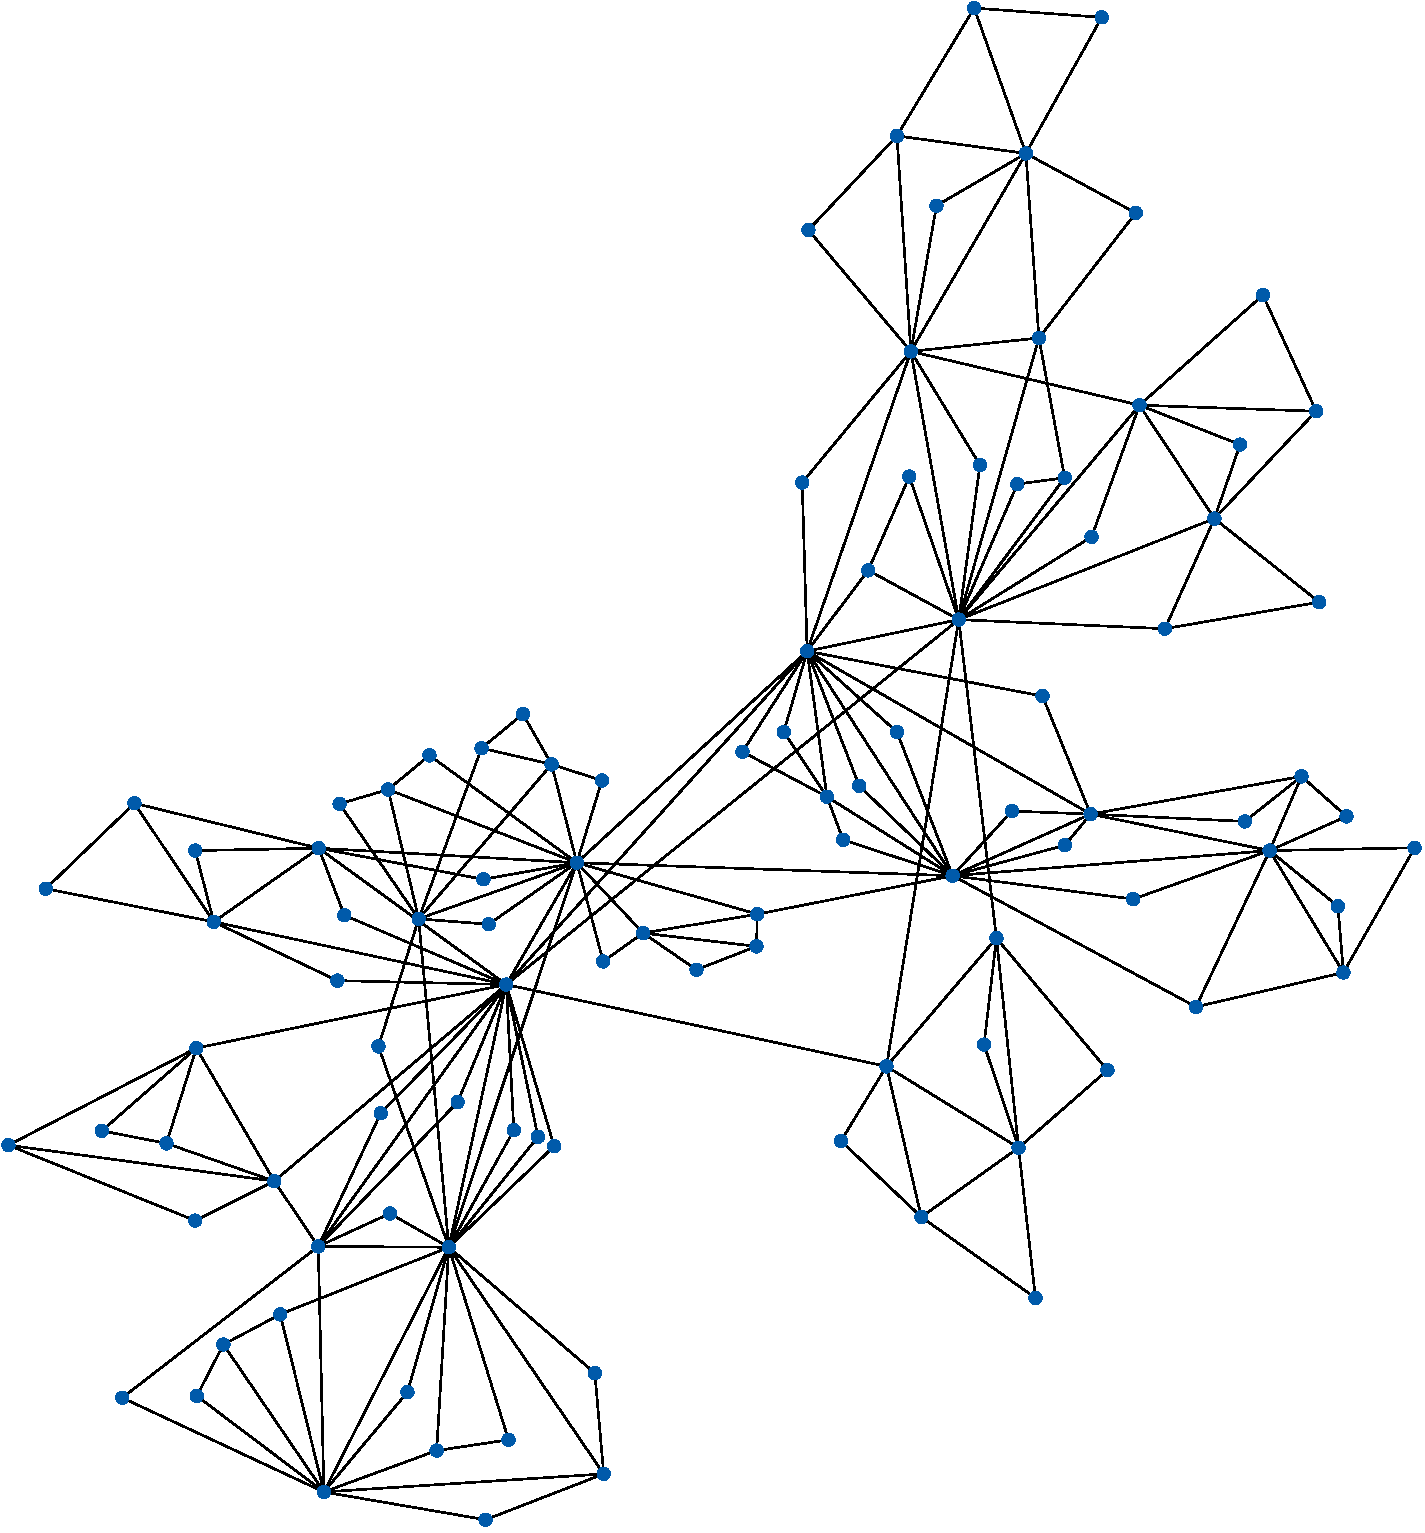
\includegraphics[width=.75\textwidth]{./img/screenshot_Dorogovtsev_Mendes.pdf}
	\caption{Représentation d'un graphe généré par l'algorithme de Dorogovtsev et Mendes possèdant 100 n\oe uds.}
	\label{fig:screenshot_Dorogovtsev_Mendes}
\end{figure}

\newpage

\paragraph{Les réseaux viaires}Enfin, nous avons également utilisé deux réseaux viaires : celui de l'agglomération du Havre et celui de l'agglomération de Rouen (voir figure \ref{fig:reseaux_viaires}). Il s'agit de graphe orienté et valué (soit par la longueur euclidienne des arcs, soit par leur temps de trajet pour les traverser). L'utilisation de deux réseaux s'est montrée intéressante car leurs structures sont très différentes l'une de l'autre. Alors que le Havre est très excentré puisqu'il est en bordure de mer, Rouen est plutôt au centre du graphe et possède un périphérique et des ponts traversant un fleuve (la Seine).

\begin{figure}[h!]
  \centering
  \subcaptionbox{Le réseau viaire du Havre - 11736 n\oe uds.}[1.\linewidth][c]{
    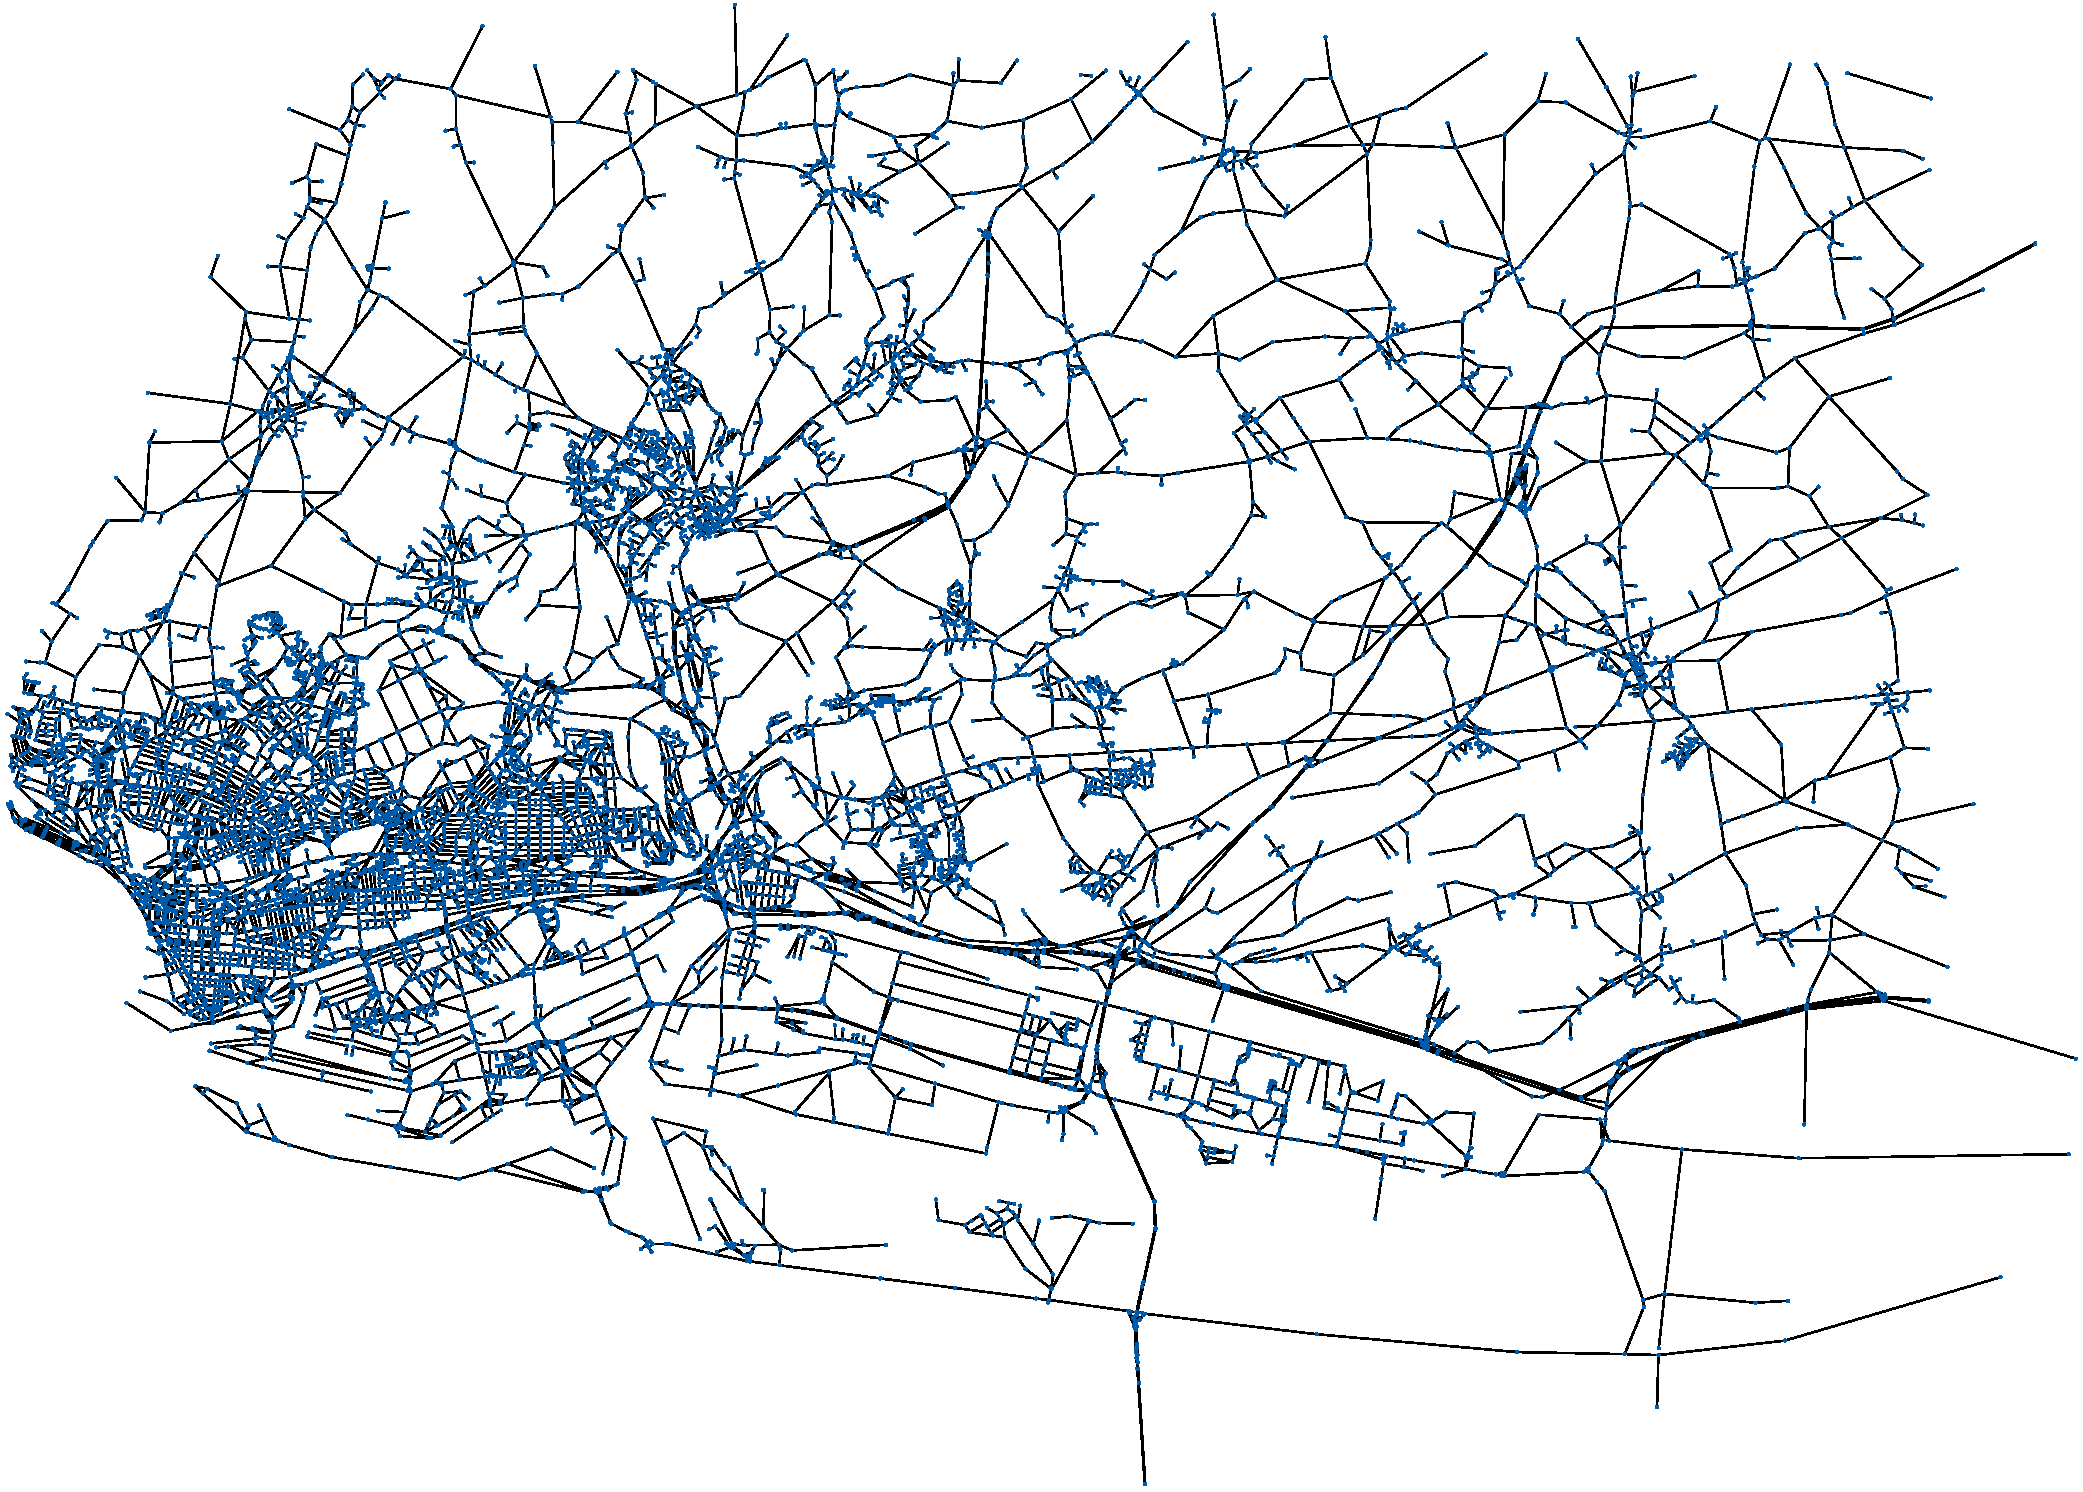
\includegraphics[width=1.\linewidth]{./img/screenshot_Le_Havre.pdf}
  }

   \subcaptionbox{Le réseau viaire de Rouen - 17442 n\oe uds.}[1.\linewidth][c]{
    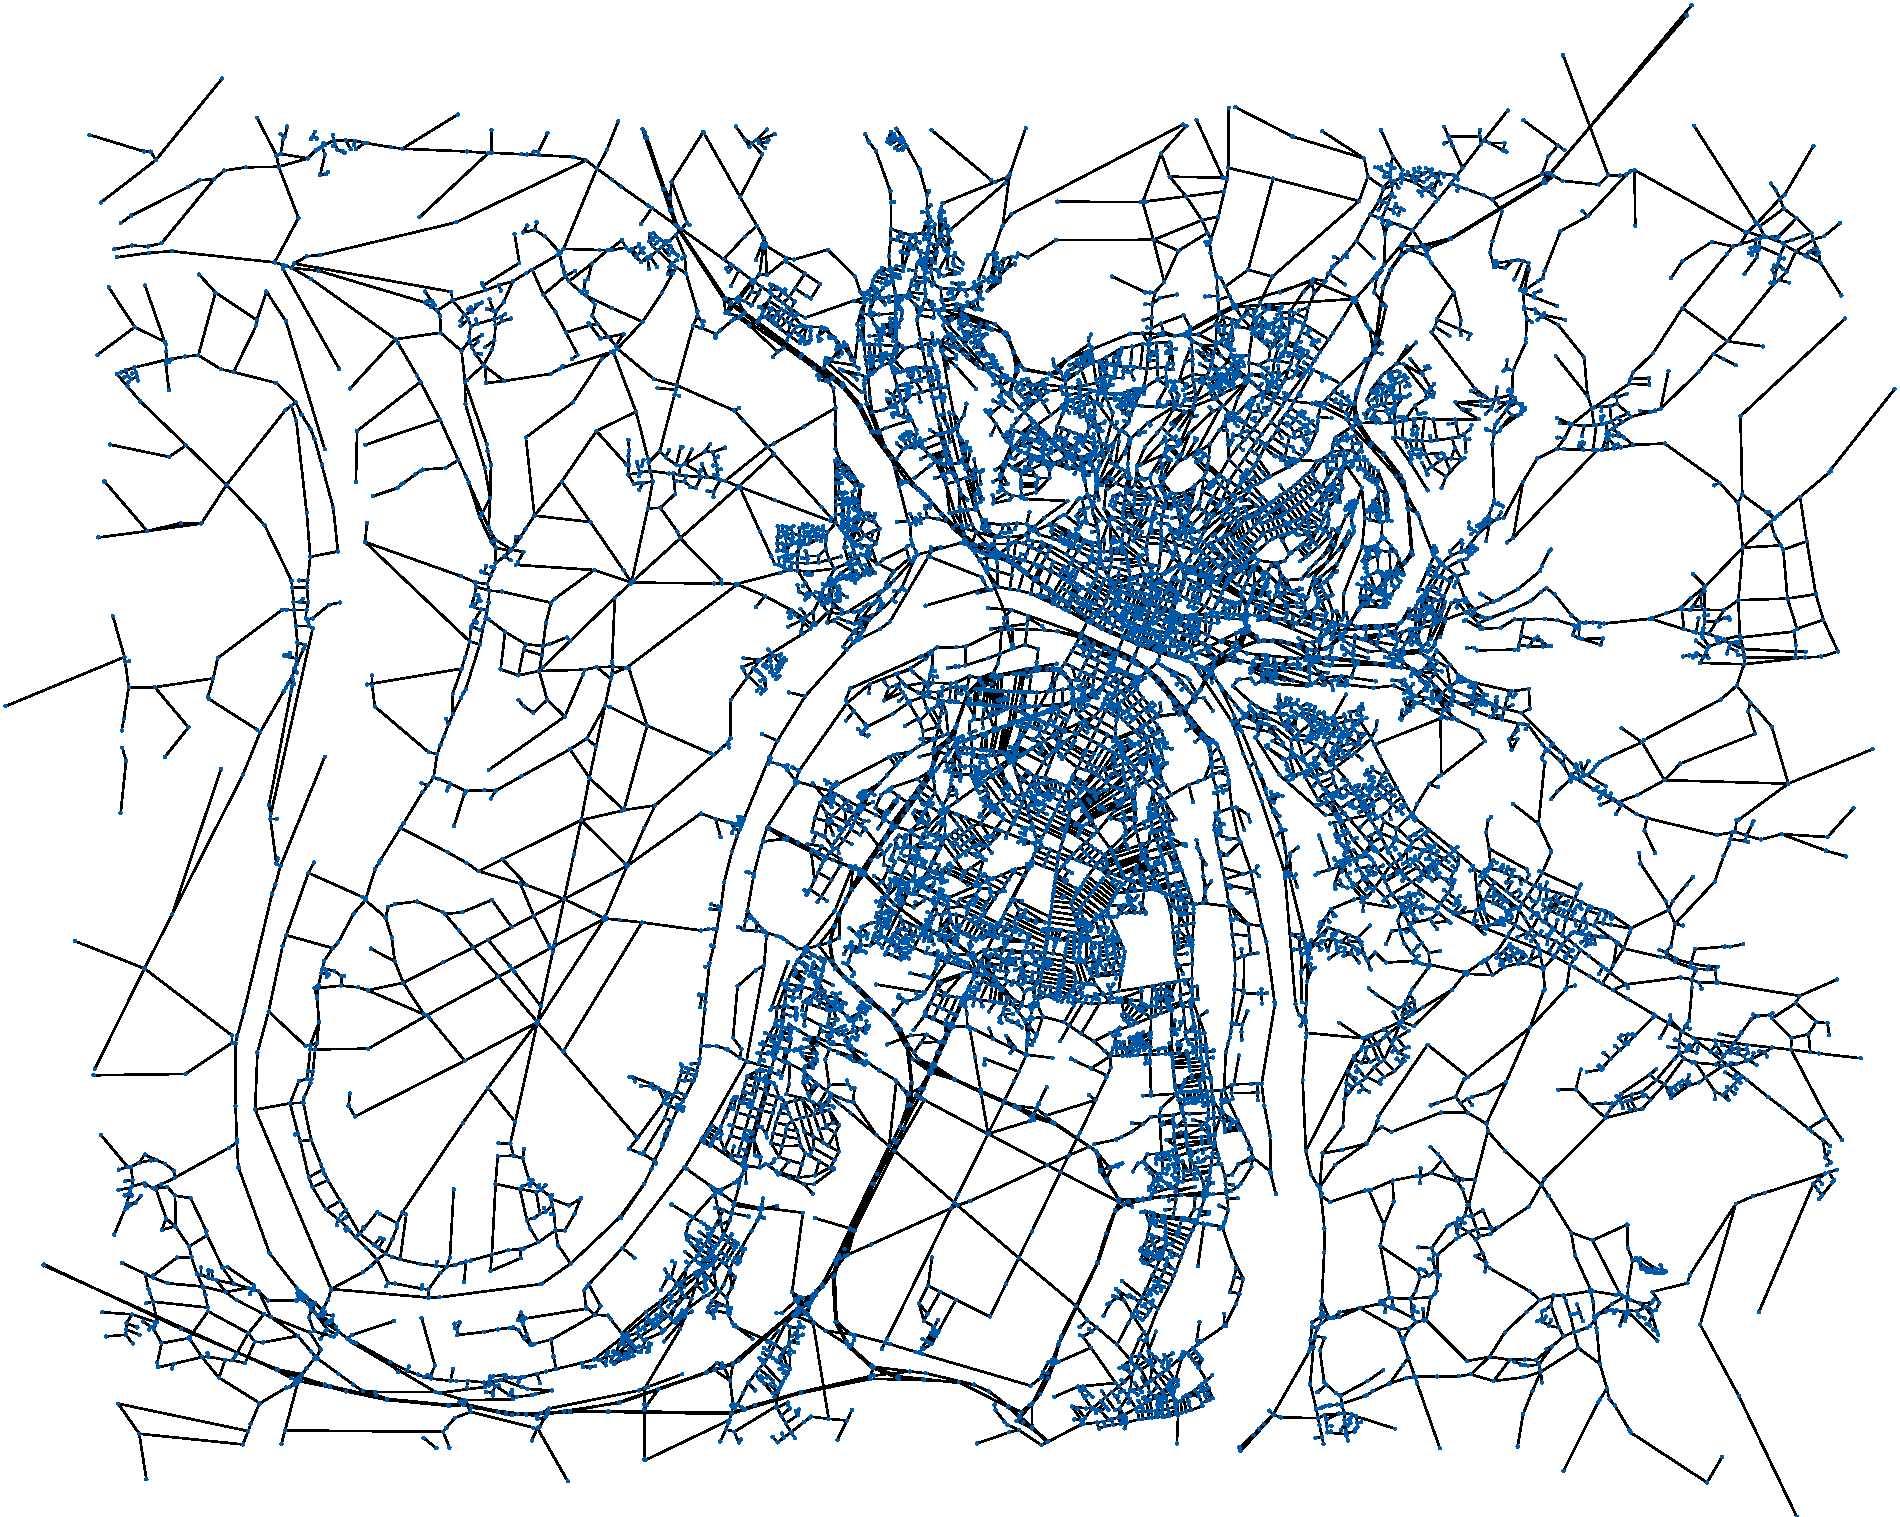
\includegraphics[width=1.\linewidth]{./img/screenshot_Rouen.pdf}
  }
  \caption{Réseau viaire de deux villes de la région.}
  \label{fig:reseaux_viaires}
\end{figure}

\chapter{Les marches aléatoires}

	\section{Les origines}

\paragraph{}Nous avons pu voir précédemment que l'information ou l'entité qui se déplace dans un graphe n'emprunte pas nécessairement un plus court chemin. Freeman, conscient de cette limite avait alors proposé un modèle basé sur les flots \cite{FreemanBorgattiWhite1991Centrality}. Mais encore une fois, nous percevons une limite car, pour emprunter le flot maximal, l'entité doit avoir conscience du "bon" chemin à prendre. 

\paragraph{}Mais qu'en est-il lorsqu'elle ne connaît pas ce chemin? Qu'en est-il lorsqu'elle possède une information incomplète, ou imparfaite du graphe? Il s'agit là de questions primordiales puisque dans un système distribué et/ou dynamique, il n'est pas toujours possible de recalculer tous les plus courts chemins, soit par manque d'informations, soit par manque de temps.

\paragraph{}Dans l'idéal, il faudrait que nous soyons en mesure de simuler avec exactitude le comportement de cette entité dans le cas distribué et dynamique. Mais bien sûr plusieurs problèmes surviennent : tout d'abord, il est parfois impossible (ou seulement trop difficile) de modéliser un tel comportement tant la complexité du système peut être importante (par exemple le modèle de déplacement d'un véhicule dans une ville); d'autre part, nous ne pouvons créer un modèle général capable de prédire le comportement adéquate pour chaque type de réseau (le mode de transfert d'information dans un réseau social, type hiérarchie dans une entreprise, est différent dans un réseau peer-to-peer).
    
\paragraph{}Afin de surmonter ces difficultés, Newman propose un modèle qui repose sur les mêmes principes que la centralité classique à la différence que les entités se déplacent selon une marche aléatoire \cite{Newman2005MeasureBetweenness} : il s'agit de la "random-walk betweenness" (que l'on peut traduire par "marche aléatoire d'intermédiarité").

\begin{figure}[h!]
  \centering
  \subcaptionbox{Résultat de la marche aléatoire sur le réseau viaire du Havre issu de la thèse de Michel Nabaa - du non emprunté en bleu clair au congestionné en rouge.}[1.\linewidth][c]{
    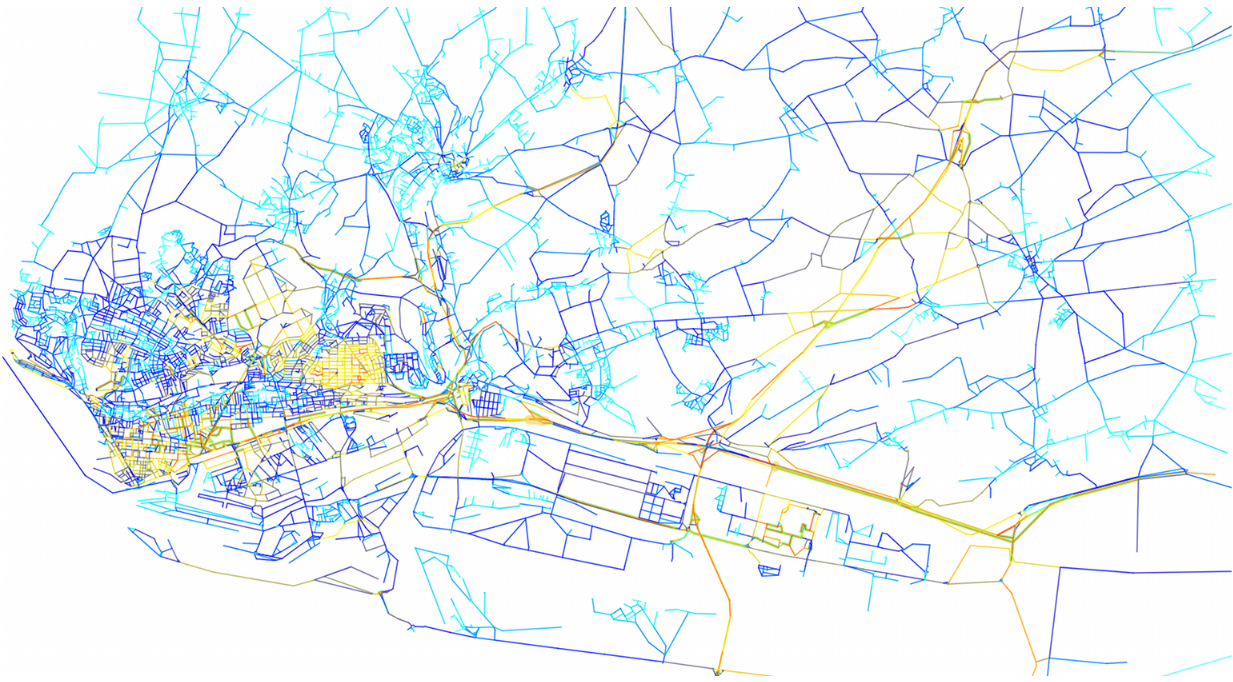
\includegraphics[width=1.\linewidth]{./img/marche_aleatoire_Nabaa_LeHavre.png}
  }

   \subcaptionbox{Résultat de la centralité intermédiaire sur le réseau viaire du Havre - de le centralité faible en bleu à la centralité forte en rouge.}[1.\linewidth][c]{
    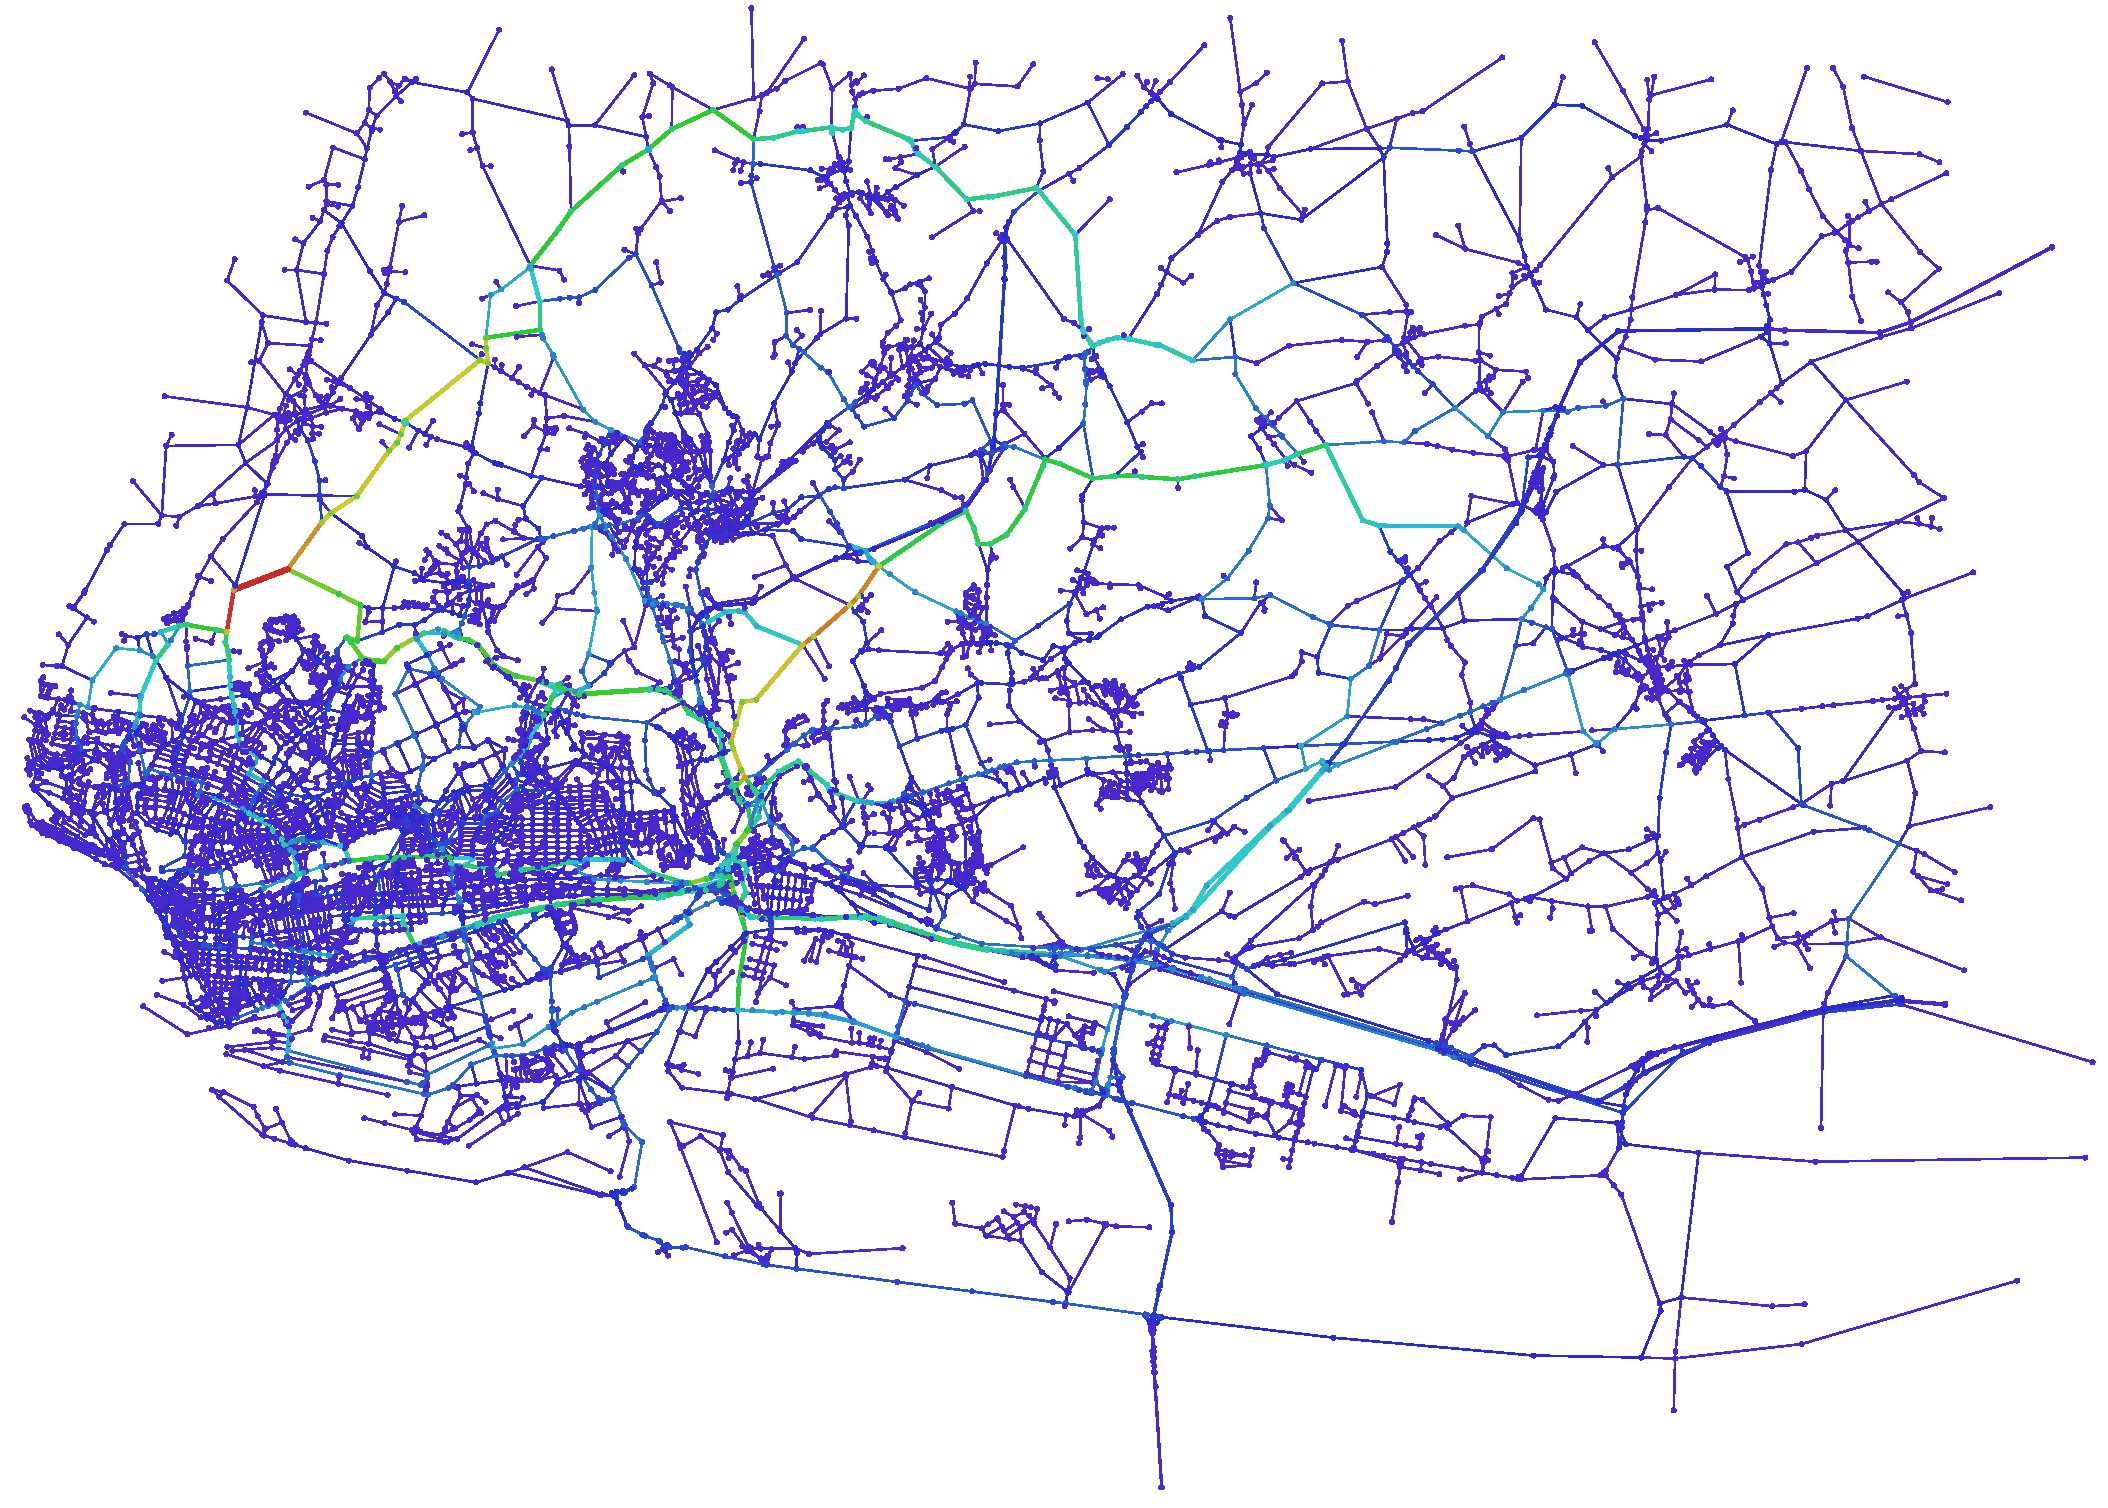
\includegraphics[width=1.\linewidth]{./img/centralite_inter_noweight_Le_Havre.pdf}
  }
  \caption{Comparaison visuelle des résultats d'une marche aléatoire et de la centralité intermédiaire. Corrélation sur les autoroutes, la Breque, l'entrée principale du Havre et la rocade.}
  \label{fig:comparaison_centralite_marche_aleatoire_nabaa}
\end{figure}

\paragraph{}D'autre part, Michel Nabaa avait mis en valeur un résultat intéressant dans sa thèse \cite{Nabaa2011Morphodyn} (voir figure \ref{fig:comparaison_centralite_marche_aleatoire_nabaa}). Il avait implémenté une marche aléatoire classique sur le réseau viaire du Havre et avait également calculé sa centralité intermédiaire. Les "marcheurs" faisaient incrémenter un compteur sur chaque n\oe ud traversé. Ainsi, par coloration du réseau, les deux méthodes semblaient mettre en valeur les même zones : notamment les autoroutes et les entrées principales du Havre.

\paragraph{}Ainsi, dans cette partie, nous avons souhaité reproduire ce résultat et mesurer avec plus de précision la corrélation entre les deux méthodes.

	\section{Le modèle}
		
\paragraph{}Ce premier modèle s'appuie sur l'implémentation d'une marche aléatoire présente dans la librairie GraphStream. Nous allons donc exposer les caractéristiques de cette marche.

\paragraph{}Nous utilisons une classe maître "RandomWalk" qui indique à chaque entité (et à chaque étape) de passer d'un n\oe ud à l'autre. Cette classe se charge également de faire évaporer une partie du score obtenu sur chaque élément du graphe (les n\oe uds et les arêtes). 

\paragraph{}Ce mécanisme nous permet d'obtenir une certaine stabilité dans les scores au bout d'un certain nombre d'itérations. Ainsi, nous avons pu mettre en place un test de stabilité qui permet de stopper automatiquement le processus lorsque la stabilité apparaît. Notons que les taux d'évaporation sont définis par l'utilisateur. Au cours de nos tests, chaque élément perdait 3\% de son score par tour.

\paragraph{}Ce test compare la valeur moyenne des éléments du graphe avec les valeurs moyennes des $x$ dernières itérations. Si la moyenne actuelle connaît un écart de plus de $y$\% avec n'importe quelle autre moyenne alors nous considérons que la simulation n'est pas stable.

Les paramètres "$x$" et "$y$" sont quant à eux définis par l'utilisateur, mais dans le cas de nos tests nous avons choisi arbitrairement $x=100$ et $y=10$.

\paragraph{}L'entité en elle-même s'inspire des mécanismes tabous. Elle ne peut retourner sur un n\oe ud qu'elle a déjà visité. Toutefois, pour éviter tout blocage, sa mémoire est limitée par un paramètre et si l'entité ne pouvait vraiment pas se déplacer sur un voisin direct, elle est capable de se "téléporter" sur un autre n\oe ud du graphe, choisi complètement au hasard.

\newpage

	\section{Les résultats}

\paragraph{}Nous observons que le modèle ne semble fournir aucun résultat correct quelque soit le type de graphe. Le tableau \ref{tab:random_walk_coef_correlation} donne les coefficients de corrélation de Pearson et de Spearman pour ces différents graphes.

\begin{table}[htbp]
	 \centering
	 \makebox[\textwidth]{
		\begin{tabular}{|>{\centering\arraybackslash}m{5.3cm}|c|c|}
			\hline
			Type de graphe                                                                      & Coef. de Pearson & Coef. de Spearman        \\
			\hline
			Dorogovtsev et Mendes \mbox{(1000 n\oe uds)}                                        &  0.2405          &  0.7412                  \\
			\hline
			Grille (10000 n\oe uds)                                                             &  0.1023          &  0.0073                  \\
			\hline
			Attachement préférentiel \mbox{(1000 n\oe uds} \mbox{et 1 arête maximum par tour)} &  0.2396          &  0.6001                  \\
			\hline
			Attachement préférentiel \mbox{(1000 n\oe uds} \mbox{et 2 arêtes maximum par tour)} &  0.3016          &  0.7217                  \\
			\hline
			Small-world \mbox{(1000 n\oe uds, $k=2$ et $\beta=0.5$)}                            &  0.2783          &  0.6392                  \\
			\hline
			Small-world \mbox{(1000 n\oe uds, $k=4$ et $\beta=0.01$)}                           & -0.0559          & -0.0158                  \\
			\hline
			Small-world \mbox{(10000 n\oe uds, $k=6$ et $\beta=0.001$)}                         &  0.0008          &  0.0214                  \\
			\hline
			Le Havre (11736  n\oe uds)                                                          &  0.3043          &  0.5540                  \\
			\hline
		\end{tabular}
	}
	\caption{Coefficient de corrélation entre la centralité intermédiaire et notre modèle de marche aléatoire pour les différents graphes.}
	\label{tab:random_walk_coef_correlation}
\end{table}

\paragraph{}Nous constatons que le coefficient de Spearman donne des résultats supérieurs à 0.6 dans certains cas. Pourtant, nous pouvons aisément affirmer grâce aux graphiques qui suivent en figure \ref{fig:graphiques_random_walk} que la corrélation n'est pas du tout significative dans ces cas là.

\begin{figure}[htbp]
	\centering
	\subcaptionbox{Dorogovtsev et Mendes (1000 n\oe uds)}[0.49\linewidth][c]{
		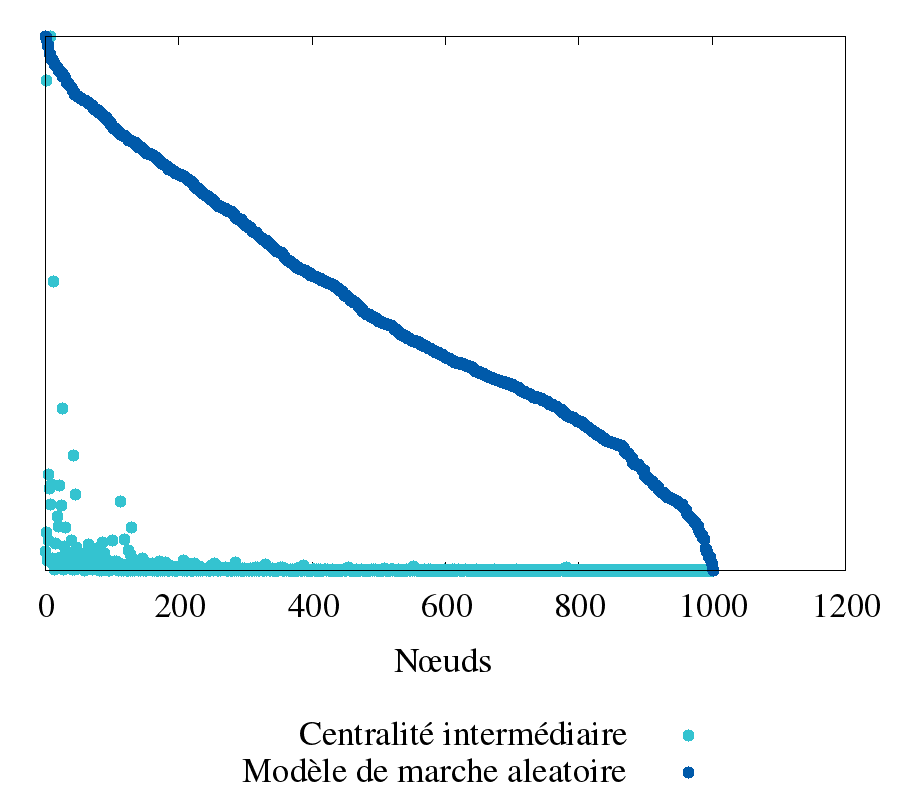
\includegraphics[width=0.49\linewidth]{./img/marche_aleatoire_dorogovstev_mendes.png}
	}
	\hfill
	\subcaptionbox{Attachement préférentiel (1000 n\oe uds et 1 arête maximum par tour)}[0.49\linewidth][c]{
		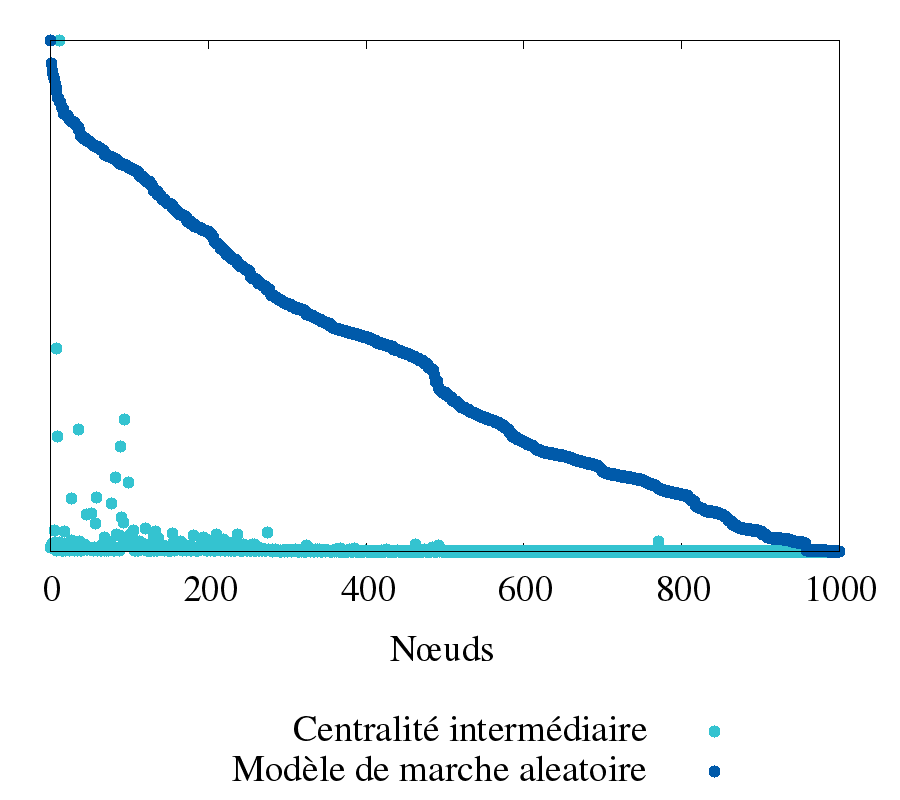
\includegraphics[width=0.49\linewidth]{./img/marche_aleatoire_preferential_attachement_1000_1.png}
	}
	\hfill
	\subcaptionbox{Attachement préférentiel (1000 n\oe uds et 2 arêtes maximum par tour)}[0.49\linewidth][c]{
		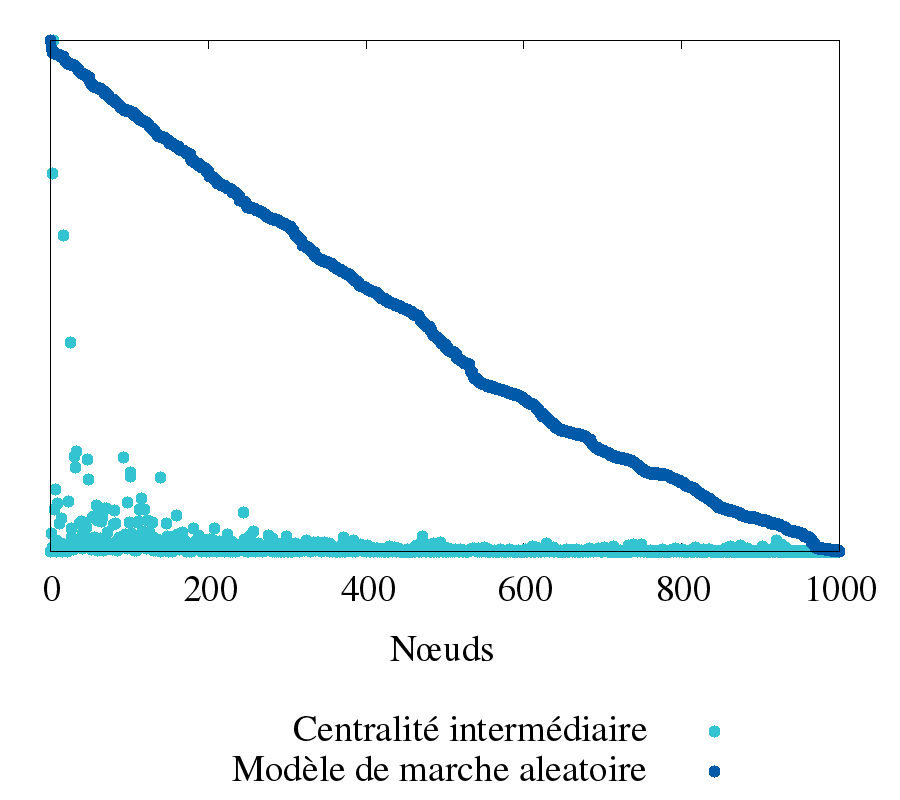
\includegraphics[width=0.49\linewidth]{./img/marche_aleatoire_preferential_attachement_1000_2.png}
	}
	\hfill
	\subcaptionbox{Small-world (1000 n\oe uds, $k=2$ et $\beta=0.5$)}[0.49\linewidth][c]{
		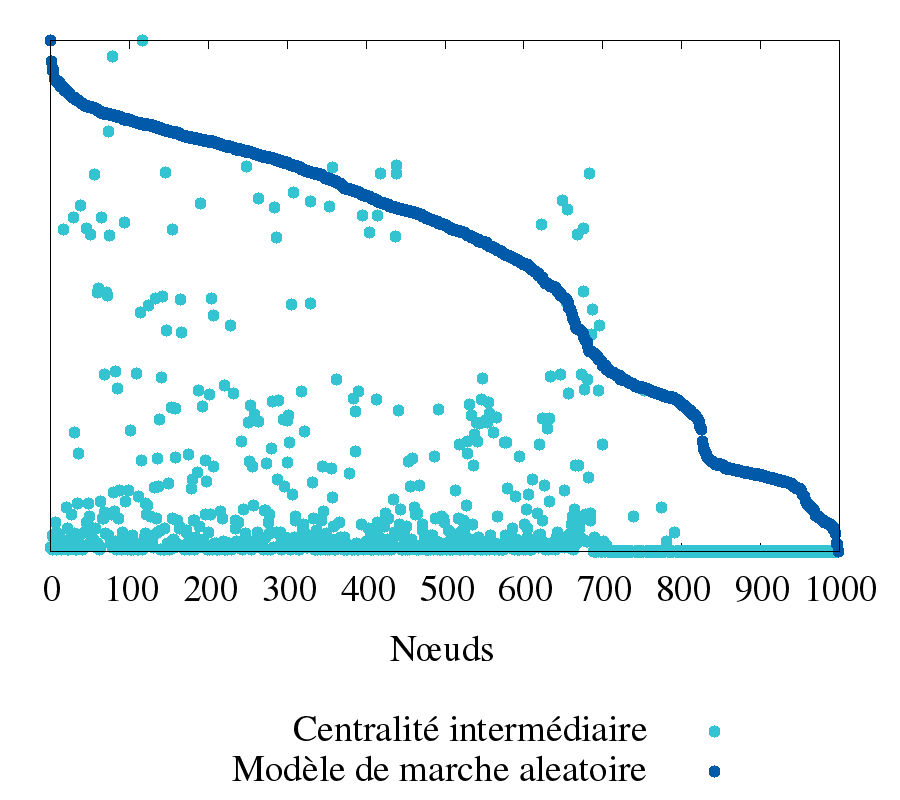
\includegraphics[width=0.49\linewidth]{./img/marche_aleatoire_small_world_1000_2_0_5.png}
	}
	\hfill
	\subcaptionbox{Le Havre (11736  n\oe uds)}[0.49\linewidth][c]{
		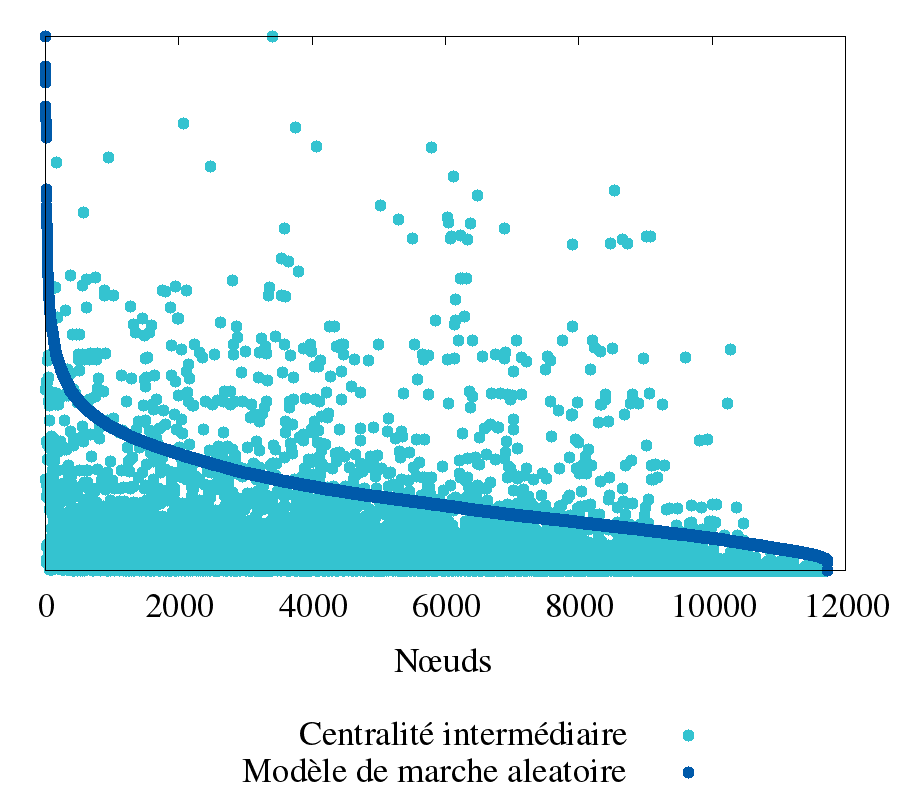
\includegraphics[width=0.49\linewidth]{./img/marche_aleatoire_le_havre.png}
	}
	\caption{Graphiques mettant en avant la non existence d'une corrélation de la centralité intermédiaire et d'une marche aléatoire. En abscisses, il s'agit de la liste ordonnée des n\oe uds selon la mesure de notre modèle; en ordonnées, les points sont situés en fonction du score obtenu par l'une ou l'autre des mesures.}
	\label{fig:graphiques_random_walk}
\end{figure}

\paragraph{}Ainsi, ce premier modèle ne permet pas de nous approcher de la centralité intermédiaire. Nous pouvons néanmoins imaginer que si les entités se déplaçaient depuis une source et vers une destination, le constat pourrait changer. Un mécanisme plus proche de la définition de la centralité serait potentiellement mieux corrélé. Nous allons donc développer dans la partie qui suit, un autre modèle dont les entités ont la particularité de naviguer entre deux n\oe uds.

\chapter{La centralité intermédiaire avec pivots}

	\section{La base du modèle}
	
\paragraph{}Afin de pallier aux problèmes soulevés dans la partie précédente, nous allons développer dans celle-ci un autre modèle plus proche de la définition initiale.

\paragraph{}Nous nous sommes inspirés de la démarche de Brandes dans \cite{Brandes2007Centrality}, où l'auteur utilise un ensemble de n\oe uds "pivots" à partir desquels, et uniquement à partir de ceux-ci, il résout des problèmes de plus courts chemins vers tous les autres n\oe uds. 

\paragraph{}Brandes montre qu'avec un ensemble de pivots suffisamment grand, nous sommes en mesure d'obtenir des résultats fortement corrélés avec la centralité classique. Cela sous-entend donc l'hypothèse que des chemins contribuent plus efficacement que d'autres. Nous supposons alors que ces chemins sont constitués de sections ayant une forte centralité. Ainsi ces sections seraient mises en valeur plus ou moins facilement avant même de finir le calcul complet.

\paragraph{}Partant de ce constat, il est possible d'émettre l'hypothèse qu'il n'est pas nécessaire de préférer une source en particulier. Effectivement, il est peu probable que toutes les paires calculées depuis un même n\oe ud source soient pertinentes. Nous supposons donc qu'il n'existe qu'un nombre limité de chemin dont la contribution est vraiment plus importante que les autres et l'existence de ces chemins est potentiellement indépendante du n\oe ud source.

\paragraph{}A priori, il peut donc être préférable de considérer des paires de n\oe uds dont les extrémités seraient choisies de manière plus uniforme sur l'ensemble des n\oe uds du graphe.

\paragraph{}Malheureusement, le calcul des plus courts chemins entre un n\oe ud source et un n\oe ud destination nécessite bien souvent de calculer les plus courts chemins partant de la source vers tous les autres n\oe uds afin de ne pas omettre un chemin moins intuitif. C'est par exemple ce que fait l'algorithme de Dijsktra. Il devient donc primordial de trouver une manière de calculer les plus courts chemins sans parcourir le graphe tout entier. 


\paragraph{}Nous avons donc choisi d'utiliser des entités dont le comportement permet le calcul de ces chemins. Ces même entités peuvent directement incrémenter le compteur de la centralité. Notre modèle se constitue donc d'un processus principal qui gère toutes les entités et leur fournit les paires de n\oe uds qu'elles doivent traiter. Voici l'algorithme de ce processus central :

\begin{algo}
Entrée : 
	- $\text{G}$ : un graphe
	- $\text{nbPaire}$ : le nombre de paire de nœuds
	- $\text{nbEntit\'e}$ : le nombre d'entité
Données :
	- $\text{listeEntit\'e}$() : la liste contenant l'ensemble des entités
Fonctions disponibles :
	- $\text{initialiserCentralit\'e}$() : initialise à zéro les compteurs correspondant à la centralité sur les nœuds
	  et sur les arêtes.
	- $\text{nouvelleEntit\'e}$() : crée et initialise une nouvelle entité
	- $\text{\'etape}$() : s'applique sur une entité et lui indique de calculer une étape de son calcul interne
Sortie : 
	- $\text{G}$ : le graphe dont les nœuds et les arêtes possèdent une pondération selon leur centralité
Début
	//Initialisation
	$\text{initialiserCentralit\'e}$()
	Pour $i$ allant de 0 à $\text{nbEntit\'e}$ faire 
		$\text{listeEntit\'e}$[i] = $\text{nouvelleEntit\'e}$()
	Fin pour
	
	//Calcul
	Tant que $\text{nbPaire} > 0$ faire
		Pour chaque $e\in \text{listeEntit\'e}$ faire
			e.étape()
		Fin pour chaque
	Fin tant que
Fin
\end{algo}

\paragraph{}De leur côté, les entités sont capables de demander au processus maître quelle paire de n\oe uds doit être traitée. Ce moment mis à part, les entités sont complètement indépendantes. Elles tracent ainsi des chemins sans cycle puis incrémentent un compteur sur chaque élément composant leur chemin.

\paragraph{}Nous allons donc expliquer dans la suite de ce chapitre trois comportements différents des entités susceptibles de résoudre notre problème. 

	\section{Le modèle avec des entités effectuant une marche aléatoire}
	
		\subsection{Le fonctionnement des entités}

\paragraph{}En développant ce premier type d'entité, nous souhaitions réunir le modèle de Brandes utilisant des pivots et le modèle de Newman utilisant des marches aléatoires.

\paragraph{}Nous avons donc créé une entité basique qui commence par récupérer une paire de n\oe uds. Partant de la source, l'entité doit, à chaque étape du calcul, choisir uniformément l'un des voisins du n\oe ud courant. Ce n\oe ud est ensuite ajouté au chemin auquel nous supprimons les éventuels cycles. Le n\oe ud courant devient alors le n\oe ud choisi et nous passons à l'étape suivante.

Lorsque l'entité arrive à sa destination, elle refait le chemin à l'envers en incrémentant le compteur sur chaque n\oe ud.

\paragraph{}D'autre part, nous avons travaillé sur des réseaux réels : le réseau routier de la ville du Havre et celui de Rouen pour corroborer nos résultats. Nous pouvions donc nous servir des données contenues sur le graphe pour réaliser des heuristiques. Par conséquent, nous avons souhaité vérifier si des entités effectuant une marche aléatoire biaisée par la distance euclidienne pouvait fournir des résultats différents.

	\subsection{Les résultats}

%
% Centralité intermédiaire par pivots et marche aleatoire
%
\paragraph{}Nous allons commencer par présenter les coefficients de corrélation obtenus avec l'entité basique.

\begin{table}[htbp]
	 \centering
	 \makebox[\textwidth]{
		\begin{tabular}{|>{\centering\arraybackslash}m{5.3cm}|c|c|c|c|}
			\hline
			\multirow{2}{*}{Type de graphe}                            & \multicolumn{2}{c|}{Coef. de Pearson} & \multicolumn{2}{c|}{Coef. de Spearman}\\
			\cline{2-5}
                                                                       & 100 paires       & 1000 paires       & 100 paires       & 1000 paires         \\
			\hline
			Dorogovtsev et Mendes \mbox{(1000 n\oe uds)}               &  0.9662          &  0.9668           &  0.7436          &  0.7531             \\
			\hline
			Grille (10000 n\oe uds)                                    &  0.9228          &  0.9368           &  0.9600          &  0.9807             \\
			\hline
			Attachement préférentiel 
			\mbox{(1000 n\oe uds} \mbox{et 1 arête maximum par tour)} &  0.9997          &  0.9999           &  0.7517          &  0.7043             \\
			\hline
			Attachement préférentiel 
			\mbox{(1000 n\oe uds} \mbox{et 2 arêtes maximum par tour)} &  0.9136          &  0.9133           &  0.8762          &  0.8743             \\
			\hline
			Small-world \mbox{(1000 n\oe uds, $k=2$ et $\beta=0.5$)}   &  0.9702          &  0.9737           &  0.9720          &  0.9692             \\
			\hline
			Small-world \mbox{(1000 n\oe uds, $k=4$ et $\beta=0.01$)}  &  0.7869          &  0.7964           &  0.5578          &  0.5748             \\
			\hline
			Small-world \mbox{(10000 n\oe uds, $k=6$ et $\beta=0.001$)}&  0.6255          &  0.6359           &  0.4985          &  0.5206             \\
			\hline
			Le Havre (11736  n\oe uds)                                 &  0.6475          &  0.6481           &  0.8628          &  0.8653            \\
			\hline
			Rouen (17442 n\oe uds)                                     &  0.5773          &  0.5805           &  0.8175          &  0.8219            \\
			\hline
		\end{tabular}
	}
	\caption{Coefficient de corrélation entre la centralité intermédiaire et notre modèle avec pivots utilisant des pivots et des entités effectuant une marche aléatoire.}
	\label{tab:centralite_pivots_marche_aleatoire_coef_correlation}
\end{table}

\paragraph{}Le tableau \ref{tab:centralite_pivots_marche_aleatoire_coef_correlation} montre clairement une corrélation plus prononcée avec ce modèle utilisant les pivots. Les coefficients de Pearson sont souvent entre 0.9 et 1.0 pour la plupart des graphes. Les coefficients de Spearman sont néanmoins plus pessimistes puisqu'ils se situent plus souvent entre 0.7 et 0.9. Nous constatons sur les graphiques de la figure \ref{fig:correlation_centralite_pivots_marche_aleatoire} que cette corrélation est significative pour les graphes dont la corrélation est forte.

\begin{figure}[htbp]
	\centering
	\subcaptionbox{Dorogovtsev et Mendes (1000 n\oe uds).}[0.49\linewidth][c]{
		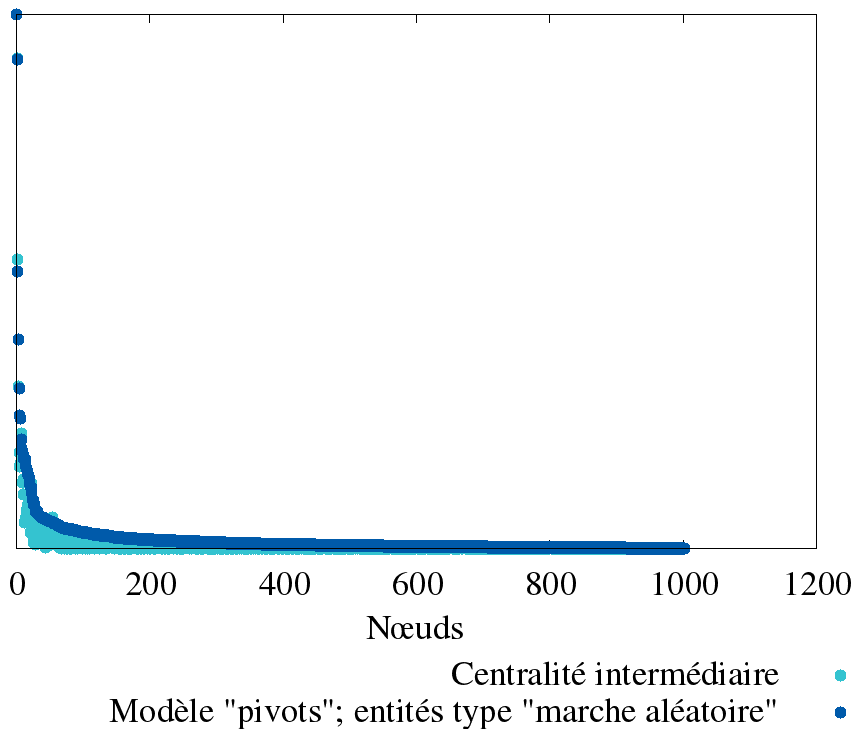
\includegraphics[width=0.49\linewidth]{./img/pivots_marche_aleatoire_dorogovstev_mendes.png}
	}
	\hfill
	\subcaptionbox{Grille (10000 n\oe uds).}[0.49\linewidth][c]{
		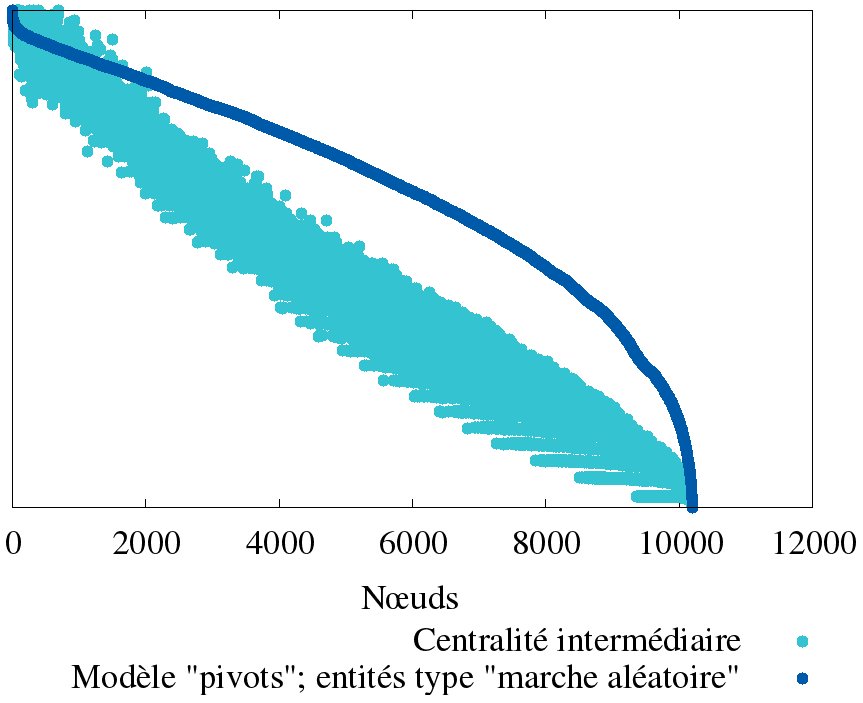
\includegraphics[width=0.49\linewidth]{./img/pivots_marche_aleatoire_grille_10000.png}
	}
	\hfill
	\subcaptionbox{Attachement préférentiel (1000 n\oe uds et 1 arête maximum par tour).}[0.49\linewidth][c]{
		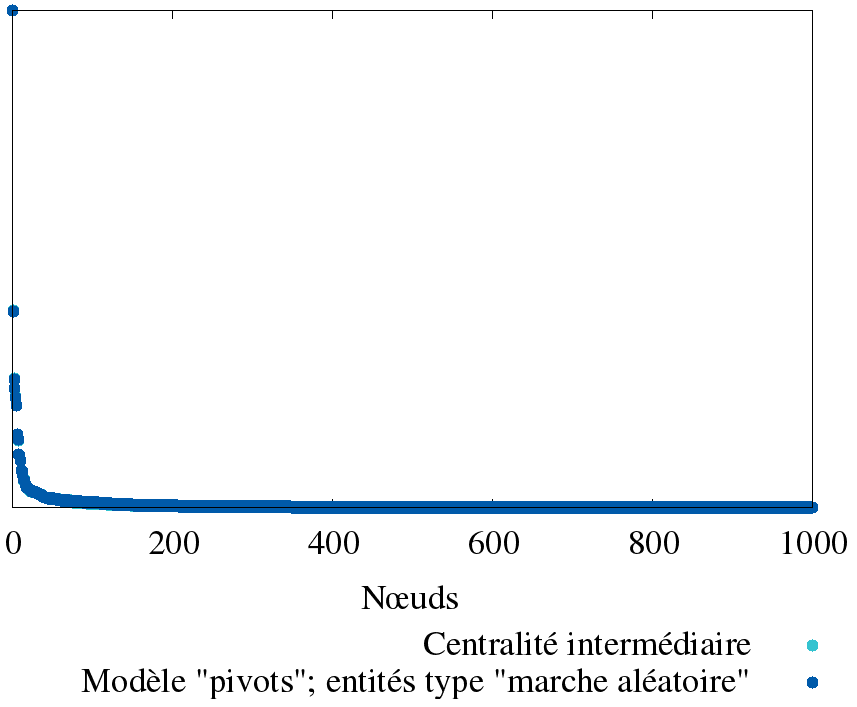
\includegraphics[width=0.49\linewidth]{./img/pivots_marche_aleatoire_preferential_attachement_1000_1.png}
	}
	\hfill
	\subcaptionbox{Attachement préférentiel (1000 n\oe uds et 2 arêtes maximum par tour).}[0.49\linewidth][c]{
		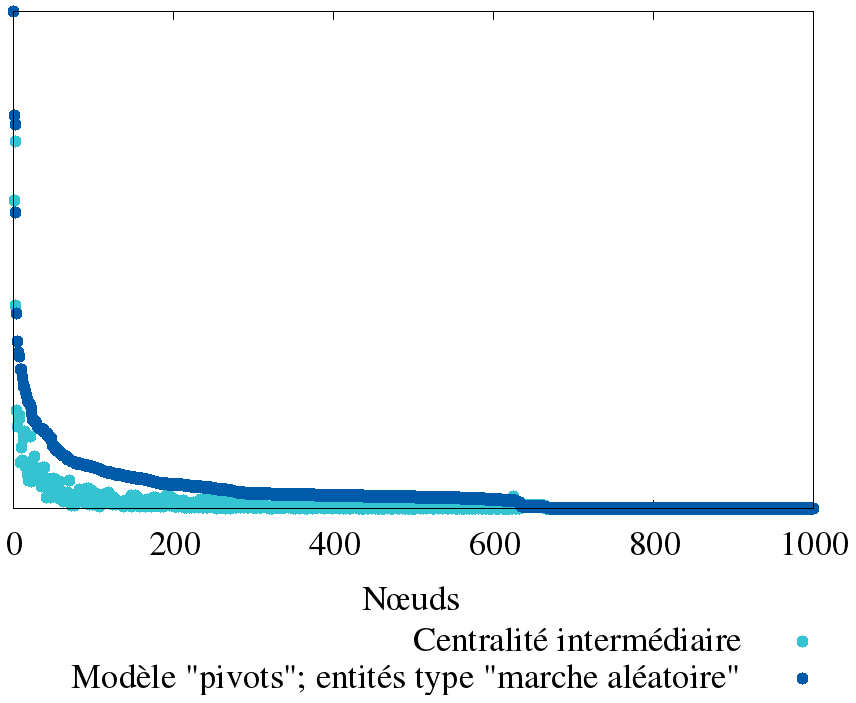
\includegraphics[width=0.49\linewidth]{./img/pivots_marche_aleatoire_preferential_attachement_1000_2.png}
	}
	\hfill
	\subcaptionbox{Small-world (1000 n\oe uds, $k=2$ et $\beta=0.5$).}[0.49\linewidth][c]{
		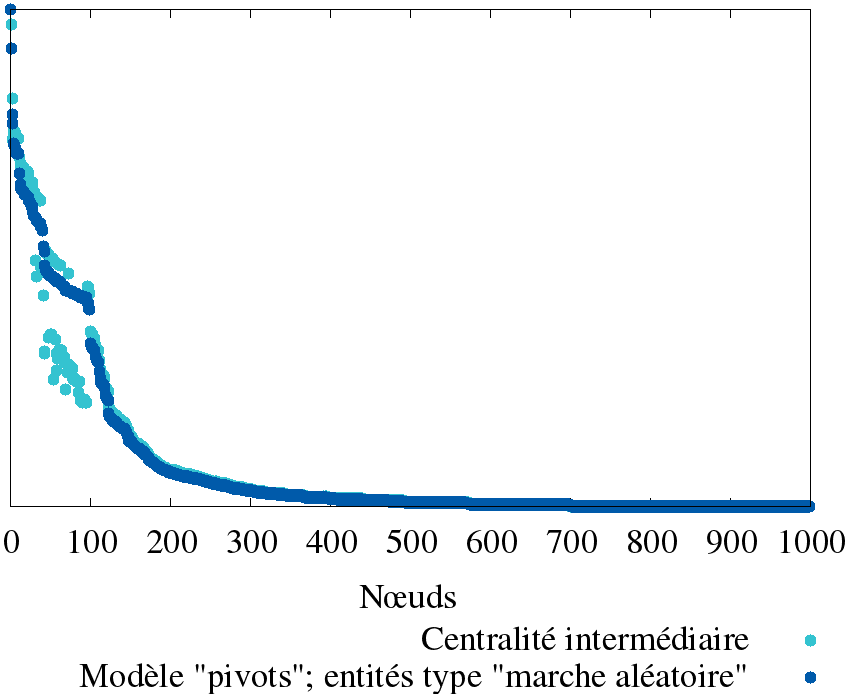
\includegraphics[width=0.49\linewidth]{./img/pivots_marche_aleatoire_small_world_1000_2_0_5.png}
	}
	\caption{Graphiques mettant en avant l'existence sur certains graphes d'une corrélation entre la centralité intermédiaire et notre modèle utilisant des pivots et des entités effectuant une marche aléatoire. En abscisses, il s'agit de la liste ordonnée des n\oe uds selon la mesure de notre modèle; en ordonnées, les points sont situés en fonction du score obtenu par l'une ou l'autre des mesures.}
	\label{fig:correlation_centralite_pivots_marche_aleatoire}
\end{figure}

\paragraph{}Il faut toutefois modérer notre propos car les résultats sur les deux derniers small-world et les réseaux viaires du Havre et de Rouen sont plutôt mauvais par rapport aux autres comme le témoigne les graphiques relatifs à ces graphes (voir figure \ref{fig:non_correlation_centralite_pivots_marche_aleatoire}).

\begin{figure}[htbp]
	\centering
	\subcaptionbox{Small-world (1000 n\oe uds, $k=4$ et $\beta=0.01$).}[0.49\linewidth][c]{
		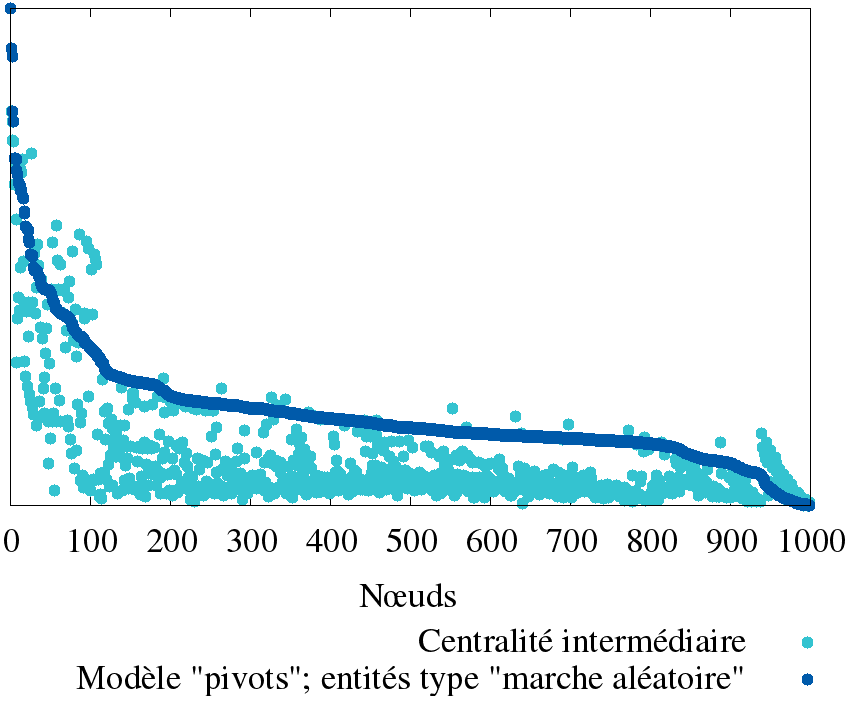
\includegraphics[width=0.49\linewidth]{./img/pivots_marche_aleatoire_small_world_1000_4_0_01.png}
	}
	\hfill
	\subcaptionbox{Small-world (10000 n\oe uds, $k=6$ et $\beta=0.001$).}[0.49\linewidth][c]{
		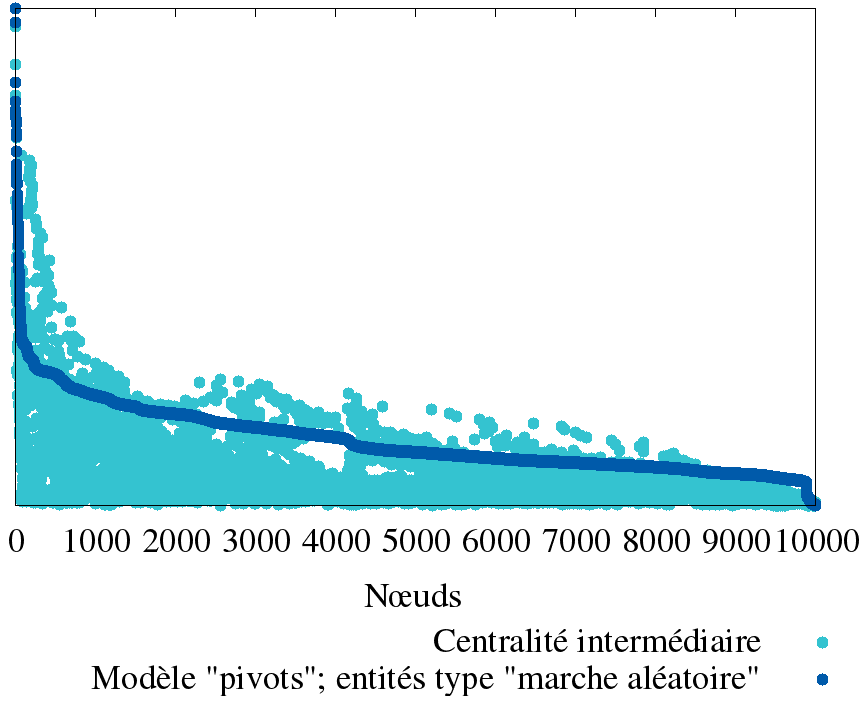
\includegraphics[width=0.49\linewidth]{./img/pivots_marche_aleatoire_small_world_10000_6_0_001.png}
	}
	\hfill
	\subcaptionbox{Le Havre (11736  n\oe uds).}[0.49\linewidth][c]{
		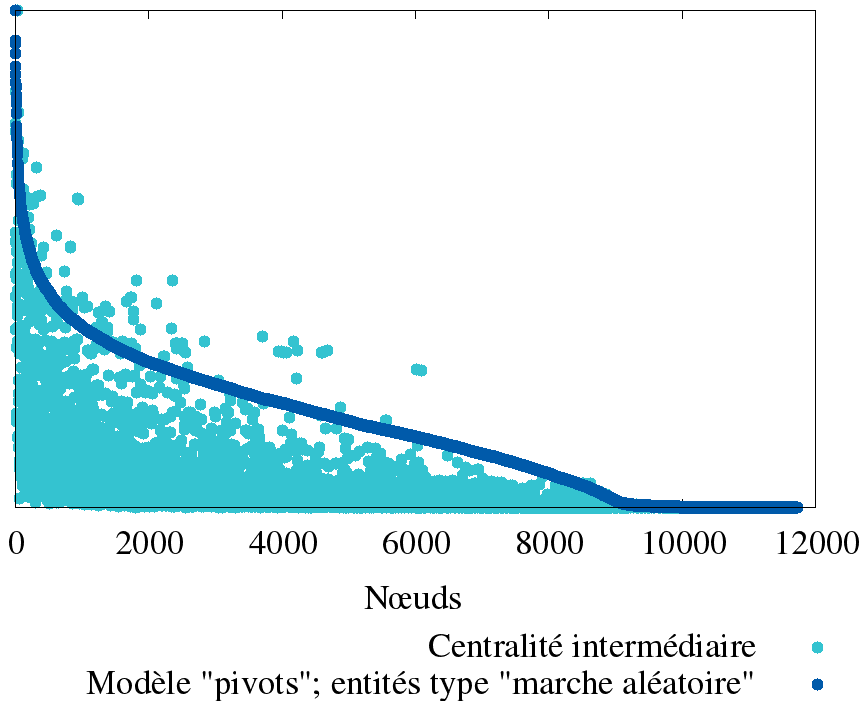
\includegraphics[width=0.49\linewidth]{./img/pivots_marche_aleatoire_le_havre.png}
	}
	\hfill
	\subcaptionbox{Rouen (17442  n\oe uds).}[0.49\linewidth][c]{
		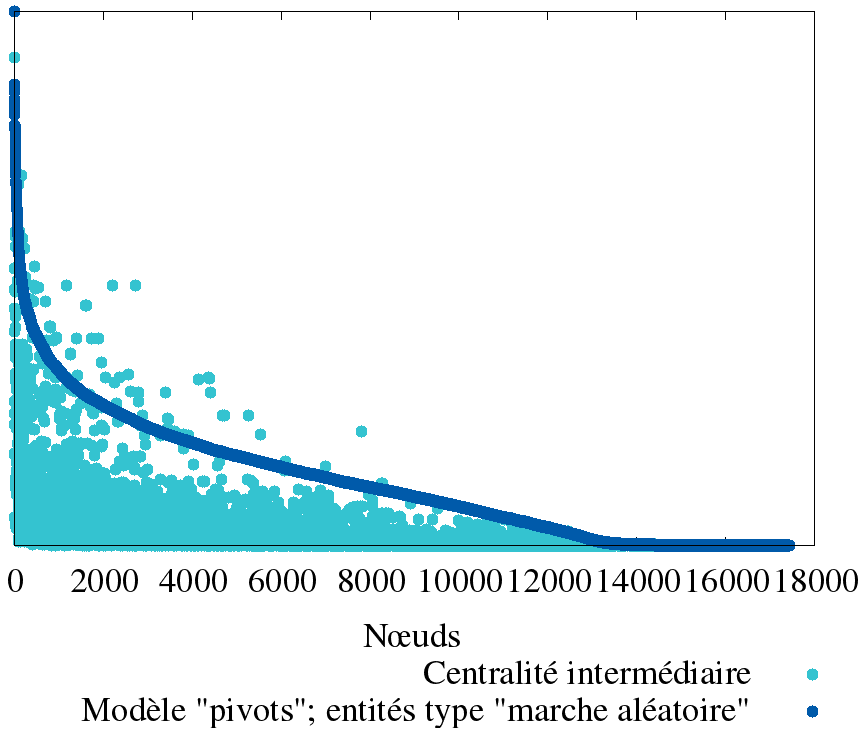
\includegraphics[width=0.49\linewidth]{./img/pivots_marche_aleatoire_rouen.png}
	}
	\caption{Graphiques mettant en avant la non-existence sur certains graphes d'une corrélation suffisante entre la centralité intermédiaire et notre modèle utilisant des pivots et des entités effectuant une marche aléatoire. En abscisses, il s'agit de la liste ordonnée des n\oe uds selon la mesure de notre modèle; en ordonnées, les points sont situés en fonction du score obtenu par l'une ou l'autre des mesures.}
	\label{fig:non_correlation_centralite_pivots_marche_aleatoire}
\end{figure}

%
% Centralité intermédiaire par pivots et marche aleatoire biaisé
%

\paragraph{}Nous allons maintenant voir si l'utilisation d'une entité biaisée permet d'obtenir de meilleurs résultats sur un réseau viaire.

\begin{table}[htbp]
	\centering
	\makebox[\textwidth]{
		\begin{tabular}{|c|c|c|c|c|}
			\hline
			\multirow{2}{*}{Type de graphe}  & \multicolumn{2}{c|}{Coef. de Pearson} & \multicolumn{2}{c|}{Coef. de Spearman} \\
			\cline{2-5}
											 & 100 paires       & 1000 paires        & 100 paires       & 1000 paires         \\
			\hline
			Le Havre (11736  n\oe uds)       &  0.6478          &  0.6517            &  0.8650          &  0.8659             \\
			\hline
			Rouen (17442 n\oe uds)           &  0.5741          &  0.5791            &  0.8170          &  0.8219             \\
			\hline
		\end{tabular}
	}
	\caption{Coefficient de corrélation entre la centralité intermédiaire et notre modèle avec pivots et des entités effectuant une marche aléatoire biaisée.}
	\label{tab:non_correlation_centralite_pivots_marche_biaise}
\end{table}

\begin{figure}[htbp]
	\centering
	\subcaptionbox{Le Havre (11736  n\oe uds).}[0.49\linewidth][c]{
		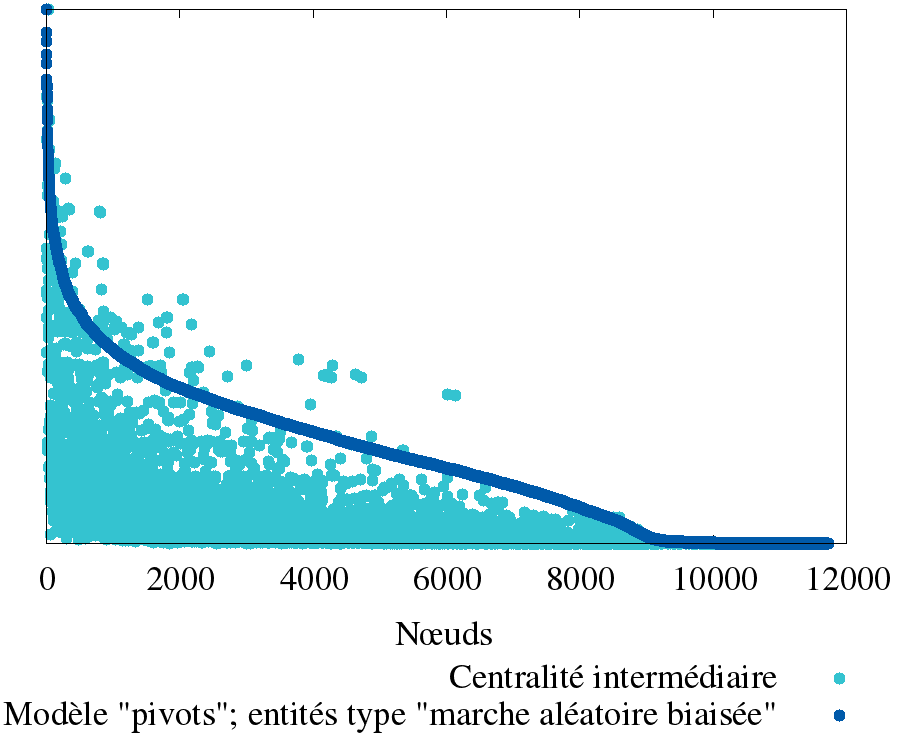
\includegraphics[width=0.49\linewidth]{./img/pivots_marche_aleatoire_biaise_le_havre.png}
	}
	\hfill
	\subcaptionbox{Rouen (17442 n\oe uds).}[0.49\linewidth][c]{
		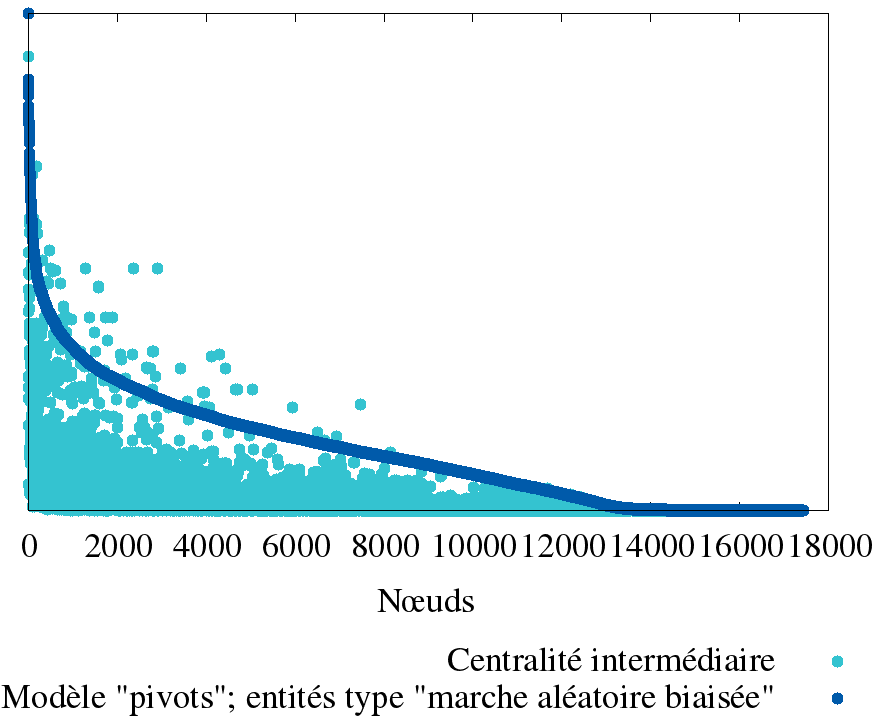
\includegraphics[width=0.49\linewidth]{./img/pivots_marche_aleatoire_biaise_rouen.png}
	}
	\caption{Graphiques mettant en avant la non existence sur les réseaux viaires d'une corrélation suffisante entre la centralité intermédiaire et notre modèle utilisant des pivots et des entités effectuant une marche aléatoire biaisée. En abscisses, il s'agit de la liste ordonnée des n\oe uds selon la mesure de notre modèle; en ordonnées, les points sont situés en fonction du score obtenu par l'une ou l'autre des mesures.}
	\label{fig:non_correlation_centralite_pivots_marche_biaise}
\end{figure}

\paragraph{}Les coefficients de corrélation du tableau \ref{tab:non_correlation_centralite_pivots_marche_biaise} se situent autour de 0.6 pour celui de Pearson, et de 0.8 pour celui de Spearman. Il s'agit grossièrement des même résultats obtenus avec les entités effectuant la marche aléatoire classique. La figure \ref{fig:non_correlation_centralite_pivots_marche_biaise} est également une représentation similaire de la marche aléatoire classique.

\paragraph{}Nous ne pouvons donc pas affirmer qu'une marche biaisée apporte un intérêt particulier. Bien sûr, le biais introduit n'est peut être pas suffisant.

\paragraph{}Pour conclure cette partie, cette méthode montre donc un certain intérêt puisqu'elle semble fournir des résultats corrects sur certains graphes. Toutefois, comme nous l'avons mis en évidence, ce n'est pas toujours le cas. Il est donc nécessaire d'approfondir le modèle. Cependant, une question se pose : est-ce que la non corrélation provient de la marche aléatoire utilisée par les entités, ou est-ce que le problème provient plutôt du mécanisme des paires qui ne serait pas pertinent?

\paragraph{}Afin de répondre à cette question, nous devons proposer une entité dont le modèle de déplacement suit d'avantage les plus courts chemins. C'est justement le point que nous allons aborder dans la partie qui suit.

\newpage

	\section{Le modèle avec des entités utilisant A\up{*}}
	
		\subsection{Le fonctionnement des entités}
		
\paragraph{}Puisque la première entité n'a pas fourni de résultats complètement concluants et notamment sur le Havre, nous avons décidé de rechercher des solutions plus proches des plus courts chemins. Tout naturellement nous nous sommes rapprochés de l'algorithme A\up{*}.

\paragraph{}Il s'agit d'un algorithme de recherche de chemin utilisant des heuristiques. Il fut présenté en premier dans \cite{Hart1968AFormalBasis} par Peter Hart, Nils Nilsson and Bertram Raphael en 1968. 

\paragraph{}Initialement, l'algorithme débute sur un n\oe ud défini par l'utilisateur. À chaque itération, A\up{*} estime un coût sur chaque voisin de son n\oe ud courant à l'aide d'une heuristique. Il stocke ainsi les n\oe uds qu'il a rencontrés dans une liste d'attente prioritaire dont l'ordre est défini en fonction de l'heuristique. L'algorithme se déplace à la prochaine étape sur le premier n\oe ud de cette file d'attente.

\paragraph{}Il boucle ainsi jusqu'à ce que le n\oe ud sélectionné soit la destination. L'algorithme est alors capable de reconstruire le chemin. De plus, si la file d'attente ne contient plus de n\oe ud avant d'avoir rencontré la destination, cela signifie qu'il n'existe pas de chemin entre les deux n\oe uds.

\paragraph{}Notre entité se contente donc de calculer le chemin à l'aide de cet algorithme et incrémente le compteur de la centralité sur chaque n\oe ud du chemin. Ci-dessous l'algorithme exécuté par l'entité au cours d'une étape.

\newpage

\begin{algo}
Données :
	- $\text{manager}$ : l'objet associé au processus maître
	- $\text{astar}$ : un objet capable d'exécuter l'algorithme A$^{*}$
	- $\text{paire}$[] : liste des deux nœuds constituants la paire
	- $\text{chemin}$[] : liste des nœuds et des arêtes constituants le chemin
Fonctions disponibles :
	- $\text{existeNouvellePaire}$() : appartient au processus maître; renvoie un booléen : 
		vrai s'il existe une nouvelle paire à calculer, faux dans le cas contraire.
	- $\text{obtenirNouvellePaire}$() : renvoie la nouvelle paire traité par l'entité.
	- $\text{calculer}$(nœudSource, nœudDest) : Calcul un chemin entre les nœuds en paramètres grâce à A$^*$
Début
	Si $\text{manager}$.existeNouvellePaire() alors
		$\text{paire}$ = $\text{manager}$.obtenirNouvellePaire()
		$\text{chemin}$ = $\text{astar}$.calculer(paire[1], paire[2])
		Pour chaque $e \in \text{chemin}$ faire
			$\text{e.centralité}$ = $\text{e.centralité} + 1 $
		Fin pour chaque
	Fin Si
Fin
\end{algo}

\paragraph{}Toutefois, cette entité ne peut en aucun cas être une solution définitive et acceptable pour le cas général. Nous souhaitions confirmer que le modèle avec les pivots pouvait fournir des résultats corrects ou si au contraire cette solution était inadaptée. Mais l'utilisation d'A\up{*} implique de posséder une heuristique admissible et monotone pour être utilisée puisque l'algorithme n'est capable de trouver le plus court chemin qu'à cette condition. Malheureusement, il est très rare de posséder une telle heuristique. 

\paragraph{}Sur un réseau routier nous pouvons nous servir d'une distance euclidienne comme heuristique si nous souhaitons un plus court chemin en terme de longueur euclidienne. Mais si nous souhaitons calculer les plus courts chemins en terme de temps de transport, alors il n'existe pas de telle heuristique. Et pour finir, sur un graphe quelconque, quelle heuristique pouvons-nous utiliser? L'algorithme risque de perdre tout son intérêt.


		\subsection{Les résultats}

%
% Centralité intermédiaire par pivots et AStar
%

\paragraph{}Nous n'allons présenté ici que les résultats sur les réseaux viaires. Les graphes virtuels générés par GraphStream ne possèdent pas de sémantique particulière. Il est donc délicat de proposer une heuristique efficace. 

\paragraph{Remarque}La centralité intermédiaire dont nous nous servons dans cette partie prend en compte la pondération des arêtes (plus précisément leur longueur). Auparavant, nous n'utilisions pas la pondération afin de pouvoir comparer avec les graphes générés par GraphStream (qui eux, ne sont pas pondérés). De plus, sur le Havre et Rouen, les résultats étaient soit équivalents, soit moins bons.

\begin{figure}[htbp]
	\centering
	\subcaptionbox{Le Havre (11736  n\oe uds).}[0.49\linewidth][c]{
		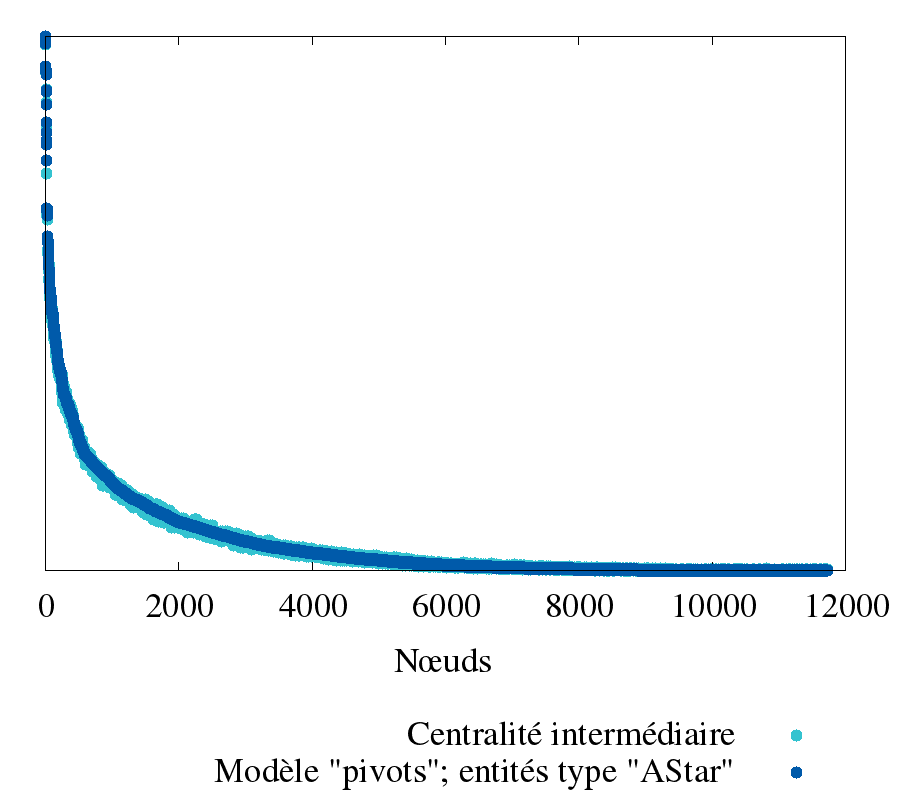
\includegraphics[width=0.49\linewidth]{./img/pivots_astar_le_havre.png}
	}
	\hfill
	\subcaptionbox{Rouen (17442 n\oe uds).}[0.49\linewidth][c]{
		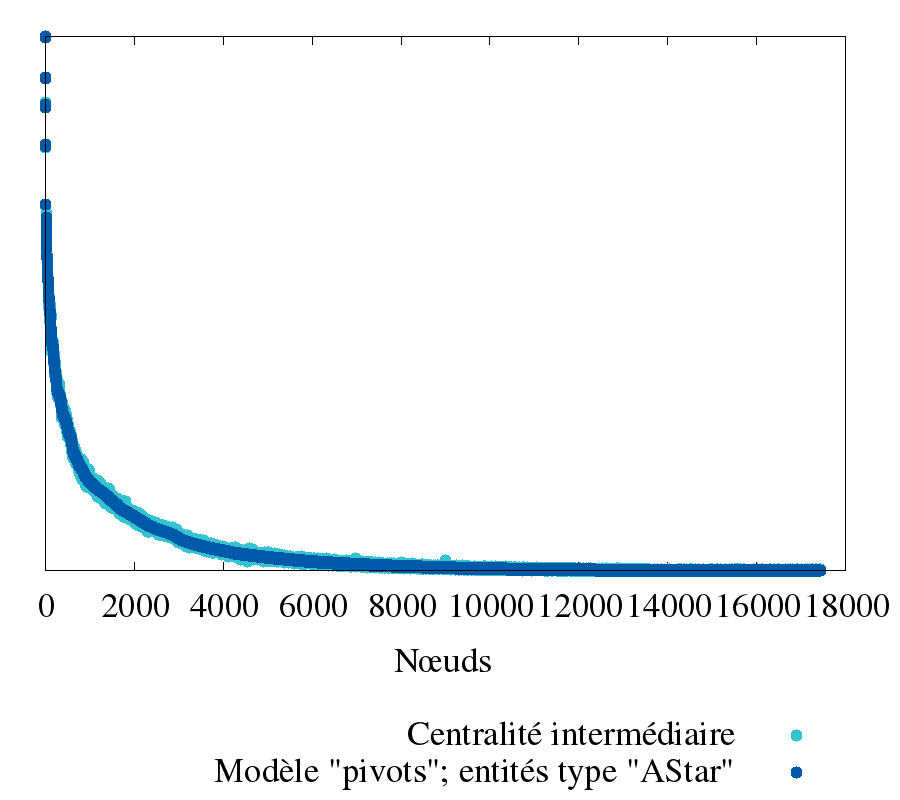
\includegraphics[width=0.49\linewidth]{./img/pivots_astar_rouen.png}
	}
	\caption{Graphiques mettant en avant l'existence sur les réseaux viaires d'une corrélation entre la centralité intermédiaire et notre modèle utilisant des pivots et des entités se servant d'A$^*$. En abscisses, il s'agit de la liste ordonnée des n\oe uds selon la mesure de notre modèle; en ordonnées, les points sont situés en fonction du score obtenu par l'une ou l'autre des mesures.}
	\label{fig:correlation_centralite_pivots_astar}
\end{figure}

\begin{table}[htbp]
	\centering
	\makebox[\textwidth]{
		\begin{tabular}{|c|c|c|c|c|}
			\hline
			\multirow{2}{*}{Type de graphe}  & \multicolumn{4}{c|}{Coef. de Pearson} \\
			\cline{2-5}
											 & 100 paires       & 1000 paires        & 10000 paires       & 20000 paires        \\
			\hline
			Le Havre (11736  n\oe uds)       &  0.8482          &  0.9817            &  0.9978            &  0.9993             \\
			\hline
			Rouen (17442 n\oe uds)           &  0.8686          &  0.9834            &  0.9986            &  0.9993               \\
			\hline
		\end{tabular}
	}
	\caption{Coefficient de corrélation de Pearson entre la centralité intermédiaire et notre modèle avec pivots et des entités se servant d'A$^*$}
	\label{tab:centralite_pivots_astar_coef_correlation_pearson}
\end{table}

\begin{table}[htbp]
	\centering
	\makebox[\textwidth]{
		\begin{tabular}{|c|c|c|c|c|}
			\hline
			\multirow{2}{*}{Type de graphe}  & \multicolumn{4}{c|}{Coef. de Spearman}   \\
			\cline{2-5}
											 & 100 paires       & 1000 paires        & 10000 paires       & 20000 paires          \\
			\hline
			Le Havre (11736  n\oe uds)       &  0.5931          &  0.9100            &  0.9897            &  0.9951               \\
			\hline
			Rouen (17442 n\oe uds)           &  0.5267          &  0.8678            &  0.9814            &  0.9912               \\
			\hline
		\end{tabular}
	}
	\caption{Coefficient de corrélation de Spearman entre la centralité intermédiaire et notre modèle avec pivots et des entités se servant d'A$^*$}
	\label{tab:centralite_pivots_astar_coef_correlation_spearman}
\end{table}

\paragraph{}Ainsi, nous constatons que les résultats de notre modèle utilisant A$^*$ sont très corrélés avec la centralité intermédiaire pour ces deux réseaux viaires. Les courbes de la figures \ref{fig:correlation_centralite_pivots_astar} se superposent quasiment, que ce soit pour le Havre ou pour Rouen. Les coefficients de corrélation des tableaux \ref{tab:centralite_pivots_astar_coef_correlation_pearson} et \ref{tab:centralite_pivots_astar_coef_correlation_spearman} indiquent également une bonne corrélation (en tout cas lorsqu'un nombre de paire suffisant est utilisé).

\paragraph{}L'utilisation de paires de n\oe uds choisies au hasard sur l'ensemble des paires possible est a priori un modèle viable. Toutefois, ce constat devra être étendu à d'autres types de graphes pour donner une affirmation définitive. De plus, comme nous l'avons exprimé dans la partie précédente, A$^*$ nécessite une heuristique pour fonctionner. Or il n'est absolument pas garanti que nous puissions en développer une. Par conséquent, il reste toujours nécessaire de trouver une entité capable de satisfaire notre exigence de plus court chemin.

\paragraph{}C'est donc pour cette raison que nous allons étudier un nouveau type d'entité dans la section suivante. 

	\section{Le modèle avec des entités "fourmis"}
	
		\subsection{Le fonctionnement des entités}

\paragraph{}Enfin, la dernière entité que nous développons actuellement se base sur les principes des colonies de fourmis. Ce concept a initialement été proposé par Marco Dorigo \textit{et al.} dans \cite{Colorni1992Distributed}. Il s'agit d'une méthode d'optimisation, ou méta-heuristique, inspiré du vivant et plus précisément du comportement des fourmis.

\paragraph{}Dans la nature, ces dernières sont capables de communiquer entre elles par le biais de leur environnement et de phéromones : nous appelons ce principe la stigmergie. Lorsqu'un ensemble de fourmis part à la découverte de son environnement pour, par exemple, rechercher de la nourriture, chaque fourmi se déplacera selon une marche plus ou moins aléatoire mais biaisée par les quantités de phéromones déjà déposées. Les fourmis laissent elles-même une certaine quantité de cette phéromone sur son passage.

\paragraph{}Le marquage de phéromone s'évaporant s'il n'est pas entretenu, nous pouvons rapidement observer l'apparition d'un chemin qu'empruntera naturellement l'ensemble de la colonie. Mais le point remarquable ici est qu'il s'agit de plus courts chemins. Ce constat a été observé par une équipe 
de chercheurs, dont faisait parti Deneubourg, et qui a rendu public ces résultats dans \cite{Goss1989Self} et \cite{Deneubourg1990Self}.

\paragraph{}Dorigo a ensuite adapté ce comportement à des fourmis virtuelles afin d'obtenir une technique décentralisée de recherche de chemin. Ce principe est aujourd'hui réputé pour s'adapter facilement à la dynamique du système. De plus, bien qu'il soit conseillé d'utiliser une heuristique, il est possible d'exécuter l'algorithme sans en avoir. Dans ce cas là, l'émergence de la solution se base sur les phéromones uniquement. Ainsi, cette solution devrait se montrer adaptée au cas général. Nous l'avons donc appliqué comme suit.

L'algorithme se déroule en différentes phases :
\begin{itemize}
    \item La construction des solutions.
    \item Le dépôt des phéromones.
    \item L'évaporation des phéromones.
\end{itemize}

\paragraph{}Selon son modèle, au cours de la construction des solutions, les fourmis parcourent un graphe de n\oe ud en n\oe ud. L'entité fourmi doit calculer une probabilité de choisir l'un des arcs adjacents à son n\oe ud courant qui dépend d'une heuristique et de la quantité de phéromones présentes sur l'arc. Nous avons éventuellement la possibilité de nous passer de l'heuristique mais l'émergence d'une solution peut être plus longue à atteindre. 

Une fois l'arc sélectionné, la fourmi se déplace dessus pour atteindre le prochain n\oe ud. 

\paragraph{}La formule de Dorigo donnant la probabilité de sélectionner un arc est la suivante : 

$$
	p_i = \frac{\tau_{i}^{\alpha}\cdot \eta_{i}^{\beta}}{ \sum\limits_{j=1}^{k}\tau_{j}^{\alpha}\cdot \eta_{j}^{\beta}}
$$
tel que :
\begin{itemize}
    \item $p_{i}$ est la probabilité de choisir l'arc $i$.
    \item $\tau_i$ est la quantité de phéromones présentes sur l'arc $i$.
    \item $\eta_i$ est une heuristique indiquant l'attractivité de l'arc $i$.
    \item $j$ est un indice qui parcourt l'ensemble des arcs à disposition de la fourmi.
    \item Enfin, $\alpha$ et $\beta$ sont des paramètres indiquant l'importance relative de la phéromone et de l'heuristique.
\end{itemize}


\paragraph{}Lors de la seconde phase, la fourmi dépose une quantité de phéromones dépendant de la formule suivante :

$$
	\tau_s = \tau_s + \frac{Q}{\text{l(C)}}
$$

tel que :
\begin{itemize}
	\item $s$ est l'un des arcs présents sur le chemin $C$ déterminé dans la première phase par la fourmi.
    \item $Q$ est un paramètre.
    \item $l(C)$ est la fonction $l$ retournant la longueur du chemin $C$.
\end{itemize}

\paragraph{}Par facilité, la dernière phase est exécutée par le processus maître. Il s'agit donc d'un processus centralisé. Nous calculons l'évaporation ainsi :
$$
	\tau_s = (1-\rho)\tau_s 
$$
tel que $\rho$ est un pourcentage d'évaporation paramétré par l'utilisateur.

\paragraph{}Pour être efficace, la construction d'une seule solution doit être menée par un nombre suffisant de fourmis et cette quantité est déterminée par expérimentation. La colonie suit donc une même phéromone pour résoudre le problème. Toutefois dans notre problème de centralité, il faut résoudre plusieurs chemins. Ainsi, nous avons adapté l'algorithme pour répondre à nos besoins. 

\paragraph{}Le processus maître définit dès l'initialisation l'ensemble des paires de n\oe uds dont nous attribuons à chacune un type différent de phéromone. L'étape au niveau d'une fourmi correspond à la création complète d'un chemin entre les extrémités d'une paire.

\paragraph{}L'ensemble des entités traite, au cours d'une même étape, la même paire de n\oe uds : d'abord la création du chemin, et ensuite le dépôt de phéromones. Puis le processus maître effectue l'évaporation sur les n\oe uds et les arêtes et fournit à la colonie la nouvelle paire.

\paragraph{}De plus, nous conservons au sein du processus maître le chemin le plus court calculé par une fourmi pour chaque paire. Ainsi, il est plus facile de parcourir les chemins, pour cette fois, de donner un score de centralité aux éléments du graphe.
	
		\subsection{Le résultat}
		
\paragraph{}Nous ne pourrons présenter dans cette partie qu'un seul résultat car le modèle n'est pas encore complètement implémenté. Le fonctionnement des fourmis ne résiste pas encore au zone "impasse". Or les deux réseaux viaires en contiennent plusieurs ce qui bloque le traitement. 

\paragraph{}De plus, nous n'avons travaillé que sur une simple grille mais pas sur d'autres types de graphes. Cela tient au fait que pour le moment la fourmi a besoin d'une heuristique alors que nous ne pouvons pas en proposer une pour les autres graphes générés. Sur la grille, l'utilisation d'une distance euclidienne ou d'une distance de Manhattan est tout à fait envisageable.

\begin{figure}[htbp]
	\centering
	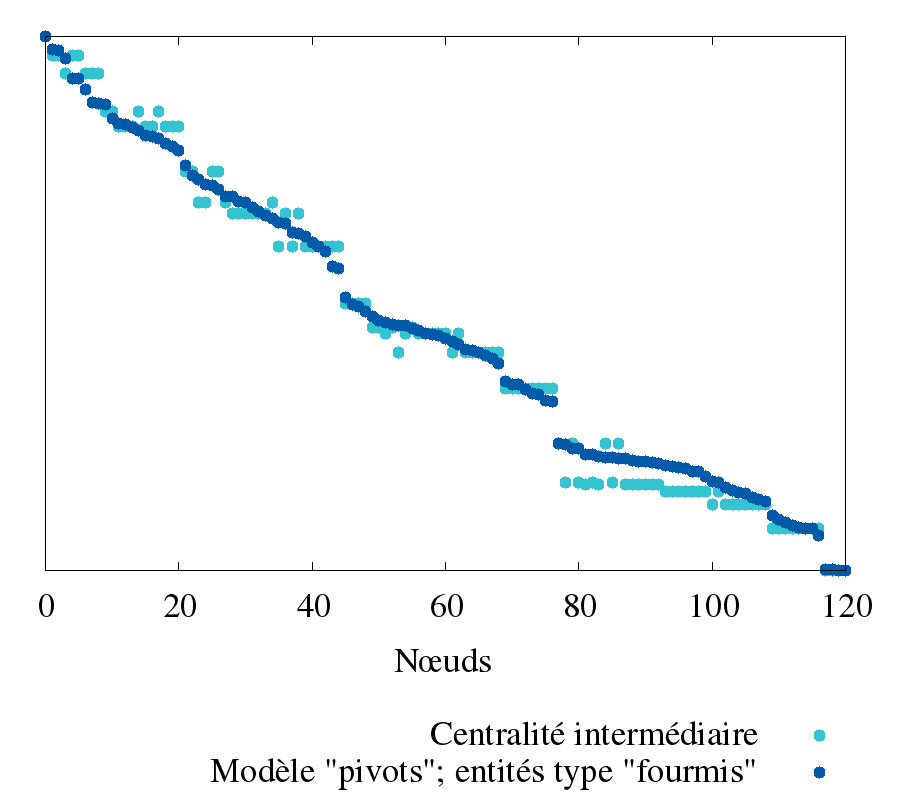
\includegraphics[width=0.65\linewidth]{./img/pivots_fourmis_grille_10.png}
	\caption{Graphiques mettant en avant l'existence sur une grille d'une corrélation entre la centralité intermédiaire et notre modèle utilisant des pivots et des entités "fourmis". En abscisses, il s'agit de la liste ordonnée des n\oe uds selon la mesure de notre modèle; en ordonnées, les points sont situés en fonction du score obtenu par l'une ou l'autre des mesures.}
	\label{fig:correlation_centralite_pivots_fourmis}
\end{figure}
	
\paragraph{}Nous constatons sur le graphique de la figure \ref{fig:correlation_centralite_pivots_fourmis} que les deux mesures sont corrélées. Bien sûr il est trop tôt pour affirmer que le modèle est viable dans le cas général mais il s'agit d'un début prometteur.


\chapter{Les perspectives}

\paragraph{}Maintenant que nous avons présenté notre modèle, nous allons expliquer les perspectives d'améliorations.

\paragraph{}Le premier point nécessitant une remise en cause est certainement l'optimisation de notre entité fourmi en lui fournissant un comportement plus complexe mais plus performant. D'ailleurs, nous avons déjà commencé d'ajouter un comportement tabou pour qu'elle soit plus robuste aux zones "impasses" présentes dans certains graphes (notamment le Havre).

\paragraph{}Le deuxième point que nous souhaiterions développer plus en détail est la méthode de sélection des paires. Nous avons préféré choisir les n\oe uds de manière complètement aléatoire car il semble difficile de considérer une stratégie en particulier sans la justifier. Ainsi, l'aléatoire est probablement la loi la plus impartiale qui soit. Toutefois, il serait très intéressant de proposer d'autres techniques de sélection. 

\paragraph{}Brandes et Pich avaient eux mêmes étudié la question dans \cite{Brandes2007Centrality} mais ils n'avaient pas nécessairement mis en valeur une méthode particulièrement plus efficace que la sélection aléatoire. 

\paragraph{}Nous sommes en tout cas en mesure d'affirmer que la centralité d'un n\oe ud doit dépendre de la structure du graphe. Mais pouvons-nous supposer qu'un graphe est constitué de clusters, et que les arêtes qui les relient sont des zones critiques où la centralité est plus forte qu'ailleurs? Si oui, il serait possible d'identifier ces clusters et de choisir des paires dont les extrémités font partie de communautés différentes. Cette méthode pourrait ainsi favoriser la mise en valeur de chemin contribuant plus efficacement au calcul de la centralité.

\paragraph{}Le troisième point à mettre en perspective se rapporte au nombre de paires utilisées. Nous avons pu remarquer au cours des tests que le nombre de paires utilisées semblait améliorer la corrélation. Nous supposons que ce nombre doit varier en fonction de la taille du graphe traité, mais il serait intéressant et utile de découvrir le rapport précis qui lie la taille du graphe et notre paramètre.

\paragraph{}Enfin, le dernier point serait de distribuer notre algorithme. Effectivement nous nous sommes efforcés de proposer un modèle auquel nous pourrions attribuer ce type de caractéristique. Mais l'implémentation peut prendre beaucoup de temps supplémentaire, donc nous avons préféré nous concentrer sur le problème principal.

\chaptertoc{Conclusion}


\paragraph{}Ce stage de recherche s'est établi dans la continuité d'un des axes d'études de la thèse de Michel Nabaa \cite{Nabaa2011Morphodyn} portant sur la centralité intermédiaire dans un réseau viaire. Cette mesure avait été utilisée pour étudier la robustesse du réseau routier de la ville de Havre. Pourtant, en cas d'accident quelconque sur le réseau, le temps de calcul nécessaire rend impossible la mise à jour de l'information dans un délai acceptable. 

\paragraph{}Puisqu'il est nécessaire de réagir vite, le sujet a consisté à proposer un modèle robuste à la dynamique (et de préférence distribuable), capable de fournir une mesure de centralité intermédiaire.

\paragraph{}En consultant les résultats de Nabaa sur le réseau du Havre, nous avons d'abord remarqué une éventuelle corrélation entre les marches aléatoires et la centralité intermédiaire. Après avoir implémenté cette marche sur différents graphes, nous avons analysé en détail la corrélation grâce aux coefficients de Pearson et de Spearman. Ces derniers ont clairement montré que les mesures ne sont pas corrélées.

\paragraph{}Nous avons donc proposé une nouveau modèle inspiré des travaux de Brandes dans \cite{Brandes2007Centrality}. Un ensemble d'entité calcule des chemins entre les n\oe uds de différentes paires sélectionnées aléatoirement sur l'ensemble des n\oe uds du graphe traité.

\paragraph{}Ce modèle a néanmoins nécessité la création de plusieurs types d'entités. Le premier correspond à une entité effectuant une simple marche aléatoire. 

\paragraph{}Nos méthodes d'analyse ont permis de mettre en avant la corrélation de notre méthode avec la centralité intermédiaire mais seulement avec quelques graphes. C'est pourquoi nous avons créé une entité utilisant l'algorithme A$^*$. Nous voulions prouver la viabilité du modèle de paire lorsque les entités effectuent des plus courts chemins. Les coefficients de corrélation nous ont rassurés dans nos suppositions puisque la corrélation était cette fois, très nette. Toutefois, A$^*$ est difficilement utilisable dans le cas général à cause de l'heuristique. Il fallait donc créer une troisième entité.

\paragraph{}Afin de garder une approche de plus court chemin, et de nous plier au besoin de dynamique, nous avons proposé une entité basée sur un comportement fourmis. Bien que cette entité ne soit pas encore pleinement fonctionnelle sur tous les types de graphes, il s'agit d'une conception prometteuse comme le témoigne le premier résultat issu du traitement sur une grille.

\paragraph{}Comme le modèle fournit des premiers résultats correctement corrélés, nous avons proposé différentes perspectives : l'amélioration du comportement de la fourmi; une méthode de sélection des paires de n\oe uds plus aboutie; la détermination du rapport entre le nombre de paires nécessaires pour une corrélation correcte et la taille du graphe; et enfin la distribution de l'algorithme.

\paragraph{}La conclusion de ce rapport de stage se termine donc après le rappel succinct des éléments clés. S'il n'y avait qu'un seul point à retenir, ce serait que la centralité intermédiaire avec pivots est une approche qui, \textit{a priori}, peut fournir des résultats corrélés avec la centralité intermédiaire classique mais qu'il est nécessaire d'approfondir ces résultats.

\bibliographystyle{ieeetr}
\bibliography{../bibliographie/biblio.bib}

\printindex

\end{document}